\documentclass[12pt,a4paper,oneside]{book}
\usepackage[utf8]{inputenc}
\usepackage[T1]{fontenc} % Better font encoding
\usepackage{lmodern} % Latin Modern fonts - more professional than Computer Modern
\usepackage{mathptmx} % Times font for text and math
\usepackage[scaled=0.92]{helvet} % Helvetica for sans-serif
\usepackage{courier} % Better monospace font
\renewcommand{\rmdefault}{ptm} % Times as default roman font
\usepackage{microtype} % Improves typography and spacing
\usepackage[margin=1in]{geometry}
\setlength{\headheight}{14.49998pt}
\usepackage{graphicx}
\usepackage{svg}
\usepackage{float}
\usepackage{amsmath}
\usepackage{amsfonts}
\usepackage{amssymb}
\usepackage{fancyhdr}
\usepackage{titlesec}
\usepackage{tocloft}
\usepackage[hidelinks]{hyperref}
\usepackage{enumitem}
\usepackage{caption}
\usepackage{subcaption}
\usepackage{booktabs}
\usepackage{array}
\usepackage{color}
\usepackage{xcolor}
\usepackage{tikz}
\usepackage{pgfplots}
\usepackage{pgfplotstable}
\usepackage{pdflscape}
\usepackage{afterpage}
\pgfplotsset{compat=1.18}

\usepackage{tabularx}

% Define column types for tables
\newcolumntype{L}[1]{>{\raggedright\arraybackslash}p{#1}}
\newcolumntype{C}[1]{>{\centering\arraybackslash}p{#1}}
\newcolumntype{R}[1]{>{\raggedleft\arraybackslash}p{#1}}

% Define professional colors early
\definecolor{chapterblue}{RGB}{23, 54, 93}        % Dark professional blue
\definecolor{CHAPTERBLUE}{RGB}{23, 54, 93}        % Dark professional blue (uppercase alias)
\definecolor{sectionblue}{RGB}{41, 84, 144}       % Medium blue
\definecolor{subsectionteal}{RGB}{58, 123, 163}   % Teal blue
\definecolor{accentgray}{RGB}{64, 64, 64}         % Professional gray

% Define vibrant DFD colors for better readability
\definecolor{entitygreen}{RGB}{46, 125, 50}       % Forest green for entities
\definecolor{processblue}{RGB}{21, 101, 192}      % Bright blue for processes
\definecolor{datastoreorange}{RGB}{255, 152, 0}   % Orange for data stores
\definecolor{flowpurple}{RGB}{156, 39, 176}       % Purple for flows
\definecolor{textwhite}{RGB}{255, 255, 255}       % White for text
\definecolor{textblack}{RGB}{0, 0, 0}             % Black for text
\definecolor{lightblue}{RGB}{227, 242, 253}       % Light blue background
\definecolor{lightgreen}{RGB}{232, 245, 233}      % Light green background
\definecolor{lightorange}{RGB}{255, 243, 224}     % Light orange background



% Custom professional title page
\begin{document}

% Custom title page
\begin{titlepage}
    \newgeometry{margin=1in}
    \centering
    
    % University Logo
    \vspace*{-1cm}
    
\includegraphics[width=2in]{RUET_logo.jpeg}
    
    % University Name
    \vspace{0.3cm}
    {\Large\textbf{\color{chapterblue}RAJSHAHI UNIVERSITY OF ENGINEERING AND TECHNOLOGY}}
    
    \vspace{0.15cm}
    {\large\color{sectionblue}Department of Computer Science and Engineering}
    
    % Main Title
    \vspace{1.2cm}
    {\LARGE\textbf{\color{chapterblue}Information System Analysis and Design}}
    
    \vspace{0.2cm}
    {\Large\textbf{\color{sectionblue}of}}
    
    \vspace{0.2cm}
    {\LARGE\textbf{\color{chapterblue}\textsc{Chorcha}}}
    
    \vspace{0.15cm}
    {\large\color{subsectionteal}An EdTech Platform}
    
    % Course Information
    \vspace{0.8cm}
    \begin{minipage}{0.8\textwidth}
        \centering
        \color{accentgray}
        \textbf{Course Code:} CSE 4110 \\[0.05cm]
        \textbf{Course Title:} Information Systems Analysis and Design Sessional \\[0.05cm]
        \textbf{Section:} A
    \end{minipage}
    
    % Students Information
    \vspace{0.6cm}
    \begin{minipage}{0.9\textwidth}
        \centering
        {\large\textbf{\color{chapterblue}Submitted By:}}
        \vspace{0.2cm}
        
        \begin{tabular}{ll}
            \textbf{Nafis Raihan} & \textbf{Roll:} 2003005 \\[0.05cm]
            \textbf{Raihan Ul Islam} & \textbf{Roll:} 2003006 \\[0.05cm]
            \textbf{Soscho Shamuel Gregory} & \textbf{Roll:} 2003007 \\[0.05cm]
            \textbf{Nahid Niyaz Shovon} & \textbf{Roll:} 2003008 \\
        \end{tabular}
    \end{minipage}
    
    % Supervisor Information
    \vspace{1.2cm}
    \begin{minipage}{0.8\textwidth}
        \centering
        {\large\textbf{\color{chapterblue}Submitted To:}}
        \vspace{0.2cm}
        
        {\large\textbf{Dr. Md. Rabiul Islam}} \\[0.05cm]
        {\textbf{Professor}} \\[0.05cm]
        Department of Computer Science \& Engineering \\
        Rajshahi University of Engineering \& Technology
    \end{minipage}
    
    % Date - positioned at bottom of page
    \vfill
    {\large\textbf{\color{accentgray}July 2025}}
    
    \restoregeometry
\end{titlepage}

% Reset page style after title page
\thispagestyle{empty}

% Table of Contents setup with professional styling
\addtocontents{toc}{\protect\thispagestyle{empty}}
\renewcommand{\contentsname}{\color{chapterblue}\Large Table of Contents}
\renewcommand{\cftchapfont}{\bfseries\color{chapterblue}}
\renewcommand{\cftchappagefont}{\bfseries\color{chapterblue}}
\renewcommand{\cftsecfont}{\color{sectionblue}}
\renewcommand{\cftsecpagefont}{\color{sectionblue}}
\renewcommand{\cftsubsecfont}{\color{subsectionteal}}
\renewcommand{\cftsubsecpagefont}{\color{subsectionteal}}
\tableofcontents

\newpage

% Title format for chapter and sections with professional colors
\titleformat{\chapter}[display]
  {\normalfont\huge\bfseries\color{chapterblue}}{%
    \colorbox{chapterblue!10}{\color{chapterblue}\Large Chapter \thechapter}}{1em}
  {\Huge\color{chapterblue}}

\titleformat{\section}[block]
  {\normalfont\Large\bfseries\color{sectionblue}}
  {\colorbox{sectionblue!8}{\color{sectionblue}\thesection}}{1em}
  {\Large\color{sectionblue}}

\titleformat{\subsection}[block]
  {\normalfont\large\bfseries\color{subsectionteal}}
  {\color{subsectionteal}\thesubsection}{1em}
  {\large\color{subsectionteal}}

\pagestyle{fancy}
\fancyhf{}  % Clear all header and footer fields
\fancyfoot[C]{\thepage}   
\fancyhead[L]{\leftmark}  % Left-aligned header (chapter name)

% Chapters
\chapter{Recognition of Need}
\thispagestyle{empty}  
\begin{figure}[H]
    \centering
    \begin{tikzpicture}
        \clip (0,0) circle(2.5cm); % Define the circular clip
        \node[anchor=center] at (0,0) {
\includegraphics[width=5cm]{banner-modified.png}}; % Image inside the circle
    \end{tikzpicture}
    \caption{Chorcha Logo}
\end{figure}
\section{Introduction}
% Circular Banner Image using TikZ

Chorcha is a leading EdTech company and Bangladesh's finest problem-solving and exam preparation site. Founded with the vision of democratizing quality education, Chorcha has established itself as a premier platform for academic excellence and skill development.

\vspace{0.5cm}

\textbf{\textcolor{chapterblue}{Company Vision:}} \\
\colorbox{chapterblue!10}{\parbox{0.95\textwidth}{\textcolor{chapterblue}{\textbf{To become the most trusted and accessible educational technology platform in Bangladesh, empowering every student with personalized learning experiences and innovative study materials that bridge the gap between traditional education and modern digital learning methodologies.}}}}

\vspace{0.5cm}

\textbf{\textcolor{chapterblue}{Company Mission:}} \\
\colorbox{chapterblue!10}{\parbox{0.95\textwidth}{\textcolor{chapterblue}{\textbf{To empower students with their optimum academic achievement through innovative study materials, comprehensive assessment tools, and a supportive online community that fosters collaborative learning and continuous improvement in academic performance.}}}}

\vspace{0.5cm}

Chorcha's flagship is a comprehensive web and mobile application platform featuring systematic mock tests, extensive question banks, previous year exam questions, and AI-based quizzes designed to prepare candidates for SSC, HSC, university entrance, and BCS exams. User experience-oriented, Chorcha provides unlimited practice tests and real-time monitoring to ensure students can achieve their academic goals with confidence and precision.

The company now serves more than 15,00,000 students, facilitating millions of practice questions and mock tests. This steady growth and extensive user engagement reflect Chorcha's solid reputation in the EdTech sector and its potential for even broader expansion in the future. However, rapid growth has also brought to the forefront limitations in Chorcha's existing information system. With the growing number of users and increasing feature complexity, there is a critical need to evaluate the existing system for scalability issues, performance bottlenecks, and process inefficiencies that could impede the company's mission.

In the context of Information Systems Analysis and Design, this chapter presents a comprehensive study of problems that impact Chorcha's systems, identifying areas requiring immediate attention to ensure future growth and sustain a high-performance user experience. By systematically identifying these problem areas, the firm can lay the groundwork for developing effective solutions that align with its strategic objectives and operational needs.

% Flowchart image
\begin{figure}[H]
    \centering
    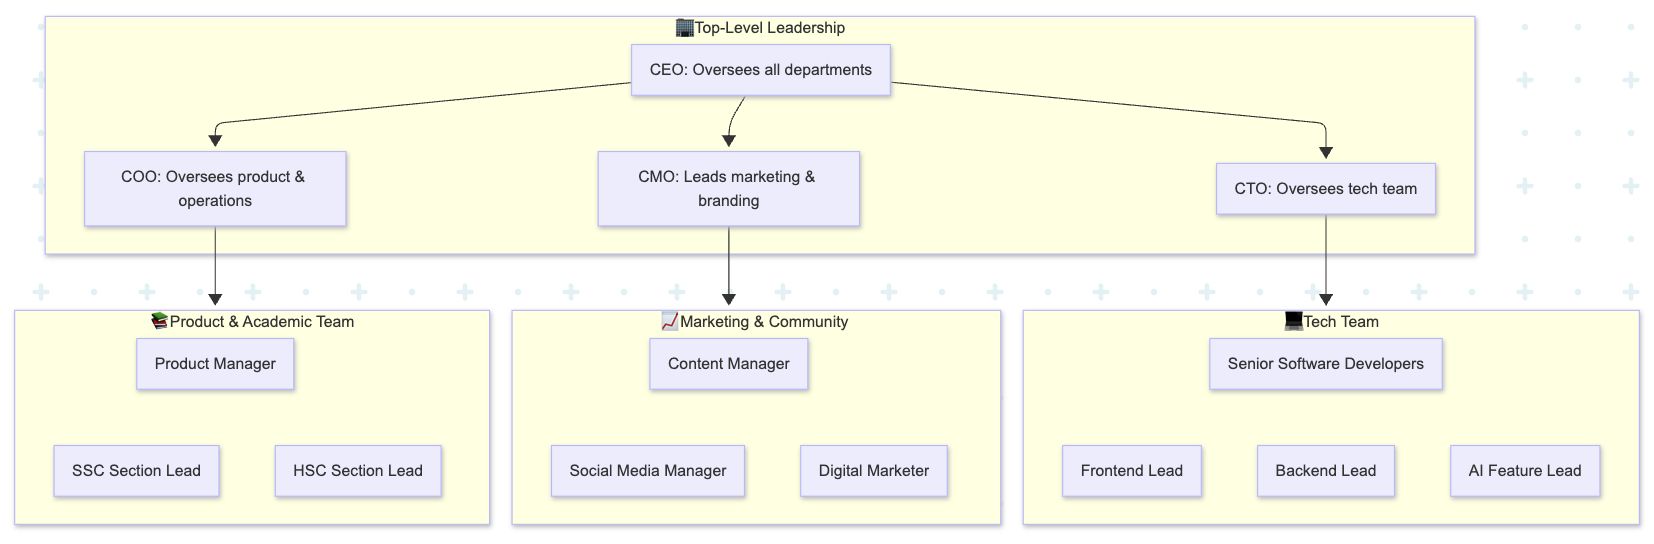
\includegraphics[width=1.0\textwidth]{flowChart4.png}
    \caption{Organizational Structure}
\end{figure}

To better understand how these challenges affect different areas of operations, it is also important to examine Chorcha's internal organizational structure. The company is managed under a leadership team that includes the Chief Executive Officer (CEO), Chief Technology Officer (CTO), Chief Operating Officer (COO), and Chief Marketing Officer (CMO). These executives oversee specialized departments such as the Tech Team, Product \& Academic Team, and Marketing \& Community Team. Each of these teams plays a critical role in ensuring content quality, platform functionality, and user engagement. However, the current structure—though functional—faces coordination challenges under rapid scale, particularly when it comes to streamlining communication between development, content, and support units. As a result, identifying and resolving system-level issues requires a cross-functional approach that aligns technical feasibility with academic rigor and operational scalability.

\newpage

\section{Problem Identification}
The following were the key problems that have been realized through detailed analysis and consultation with stakeholders:

\subsection{Problem 01: Scalability Challenges in Manual Evaluation of Subjective Responses}
\textbf{Elaboration:} The grading of written or subjective questions, e.g., Bengali/English answers or descriptions of Chemistry, is still manually verified by moderators or teachers. With the growth in users and the rise in exam answers, the manual verification process has become extremely inefficient and unscalable. As the number of users increases, delays in evaluation are accelerated, causing delayed feedback for students. This causes declined motivation among users, as they receive inadequate timely or frequent feedback, which lowers the user experience and platform trust.

\subsection{Problem 02: High Volume of User-Reported Confusing Questions}
\textbf{Elaboration:} Chorcha currently deals with more than 100,000 examinations on a daily basis, and with such a large quantity, students tend to report "incorrect" or "perplexing" questions. Although most reports are legitimate, manually reading every report is too overwhelming a task for the moderators and administrators. The large quantity of reports not only saturates the system but also leads to delays in the resolution of legitimate issues, that undermine the trust in the quality of the content provided. Without an efficient system with which to deliver these reports, the platform risks losing credibility and user satisfaction by means of unresolved or inappropriately long going issue resolution.

\subsection{Problem 03: No Offline Mode or Low-Bandwidth Adaptation}
\textbf{Elaboration:} The majority of users of Chorcha are rural in location, where internet connections are erratic or slower. This is problematic for students who rely on the platform to access examinations and study materials, as the platform does not support offline at the moment. If users encounter network downtimes, their experience is disrupted, particularly during exams, that leads to a poor user experience. This also reduces retention rates, particularly in Tier-2 and Tier-3 regions, where the internet connectivity tends to be unstable.

\subsection{Problem 04: Performance Bottlenecks During Peak Usage}
\textbf{Elaboration:} During peak usage times, the system experiences slowdowns that and thereby have a direct impact on user experience. Specifically, features such as mock tests and real-time transactions suffer from high latency. With so many students simultaneously utilizing the platform, bottlenecks are faced, and the system's performance is hampered. Such hampering of performance during times of heavy usage not only annoys users but also threatens to deter them from exiting the platform for better scalability and reliability-based alternatives.

\subsection{Problem 05: Challenges in Testing and Quality Assurance}
\textbf{Elaboration:} Chorcha currently relies on manual testing for frontend and UI components, which is time-consuming and error-prone. With the growing complexity of the platform and the increasing number of features, the manual testing approach has become inefficient and unreliable. The risk of bugs and errors being overlooked during manual testing can lead to a diminished user experience, especially when users encounter errors in the middle of exams. The platform needs an automated solution that has broader coverage, reduces human error, and streamlines the development cycle.

\section{Conclusion}
The recognition of these problems speaks to the necessity of an organized and comprehensive process to bolster Chorcha's information system. All of the issues that have been discovered – from manual evaluation scalability problems to performance hiccups at peak usage – may hinder the company's growth as well as the service quality being provided to users. Resolving them is therefore not just an operational necessity but strategic for Chorcha to maintain success within the competitive EdTech space.
\\ \\By strategic improvements such as a move towards AI-powered assessment, implementing question trust scoring mechanism, adopting Progressive Web App (PWA) technology for offline support, optimization of performance using load balancing and caching, and automated testing, Chorcha can significantly enhance the efficiency, scalability, and reliability of its system.
\\ \\These enhancements will not only automate steps and reduce human intervention but also dismantle silos and make the platform scale well to support higher demand. Secondly, these upgrades will increase user satisfaction, keep students in underserved communities, and improve confidence in the platform. The findings generated in this needs analysis form the setting to consider appropriate solutions, which are discussed in the next chapter, and eventually contribute to the design of a more effective information system for the firm's future.

\newpage

\chapter{Initial Feasibility Study}
\thispagestyle{empty}  
\section{Introduction}
A feasibility study is a critical milestone in information system analysis and design because it determines the practicability and feasibility of proposed solutions before their implementation on a wide scale. This chapter examines how Chorcha can address the problems discussed in the previous section by taking into consideration various solution alternatives alternatives and weighing them against factors such as cost, time, technical
complexity, and resource requirements. The objective is to arrive at the proposed solutions that are feasible and most desirable for Chorcha in the short term and long term. By thorough analysis of economic, operational, technical, and schedule factors for every problem identified, Chorcha's development team and management can make informed decisions on further action. We provide the detailed preliminary feasibility study of each important problem area, reporting findings and recommendations to direct the subsequent system design and implementation phases.

\section{Initial Feasibility Analysis}

\subsection{Problem 01: Scalability Challenges in Manual Evaluation of Subjective Responses}
\textbf{Statement of the problem:} Manual evaluation of subjective responses is not scalable when the user base rises.\\ \\
\textbf{Summary of findings:} The current manual evaluation system is incapable of handling the rapid scale at which user submissions are growing. Implementing an AI-based evaluation engine will not only significantly reduce the evaluation time but also improve consistency in grading and user feedback. Moreover, it will unlock the ability to offer real-time or near real-time assessment for subjective content, thus transforming the feedback loop into a highly responsive and motivating component of the learning cycle.
\\ \\
\textbf{Details of findings:}
\begin{itemize}
    \item \textbf{Current evaluation process:} Manual checking of subjective answers is slow and inefficient, particularly with growing users.
    \item \textbf{Solution benefits:} AI-powered assessment will speed up marking, remove human mistakes, and provide more consistent feedback.
    \item \textbf{Challenges:} Entails significant investment in AI and NLP model building. Ensuring accuracy and fairness in marking could be challenging.

    \item \textbf{Testing and validation:} AI marking must be trained on teacher-marked data in order to maintain quality and consistency.
\end{itemize}
\textbf{Recommendation:} Use AI-powered assessment with NLP models fine-tuned on current data. This remedy will enable Chorcha to scale the grading process efficiently and deliver more consistent feedback. Flagging ambiguous answers
for human evaluation as well also guarantees that subjective subtleties are not lost,improving the accuracy and impartiality of assessments. Machine learning algorithms will not only hasten the evaluation process but will also make it possible Chorcha to provide a high quality of feedback so as to enhance user satisfaction and long-term student retention.

\subsection{Problem 02: High Volume of User-Reported Confusing Questions}
\textbf{Statement of the problem:} Large numbers of students report "wrong/confusing questions," which is not possible to manually examine each report one by one.\\ \\
\textbf{Summary of findings:} Manual moderation of large volumes of question reports has proven unmanageable. The introduction of a question trust scoring system powered by AI can filter out less significant reports and focus on identifying critical content issues. This mechanism, by analyzing patterns and report frequency, will ensure better prioritization, improve moderator efficiency, and help maintain high content quality without overwhelming the human review pipeline.\\ \\
\textbf{Details of findings:}
\begin{itemize}
    \item \textbf{Current system overload:} Moderators are inundated with reports,resulting in delay and loss of confidence.
    \item \textbf{Solution benefits:} The trust scoring with AI will make sure to only verify frequent and low-confidence questions. The user trust will also be preserved.
    \item \textbf{Challenges:} Designing AI with crowd agreement may be complex, and accurate scoring must be guaranteed.
    \item \textbf{Testing and validation:} Track user feedback and complaints to enhance the trust scoring mechanism regularly.

\end{itemize}
\textbf{Recommendation:} Deploy the question trust scoring system to focus on refeedback-based and precise perception. Overload of moderators will be avoided by the system so that they can focus on the most critical issues. Adding AI-generated explanations will also make questions even more clear before they get flagged, so users won't get confused initially. Such advanced content review will reduce manual intervention to a great extent, streamline processes, and maintain the platform authentic by resolving user concerns in a timely manner and in the right way.

\subsection{Problem 03: No Offline Mode or Low-Bandwidth Adaptation}
\textbf{Statement of the problem:} Students in rural areas struggle with consistent access.\\ \\
\textbf{Summary of findings:} In low-bandwidth and rural environments, lack of offline support severely limits user engagement. Implementing Progressive Web App (PWA) technology with offline capabilities will ensure that all students—regardless of internet availability—can access core learning and testing features. It will empower students to learn on their own time and sync automatically when reconnected, improving accessibility and inclusivity in remote regions.\\ \\
\textbf{Details of findings:}
\begin{itemize}
    \item \textbf{Current limitations:} Rural students have connectivity, leading to broken experiences and decreased engagement.
    \item \textbf{Solution benefits:} PWAs support offline modes and automatic syncing, which is ideal for low-bandwidth environments.
    \item \textbf{Challenges:} Development of offline support and syncing vast exam data can turn out to be resource-intensive.
    \item \textbf{Testing and validation:} Perform real-world testing in low-bandwidth areas to ensure that offline modules function perfectly.
\end{itemize}
\textbf{Recommendation:} Implement a Progressive Web App (PWA) with offline exam support and a synchronization feature. This resolution will provide assurance that rural or low-bandwidth area users can access exams and study material uninterruptedtion. It will help retain students that otherwise cannot participate in exams during network downtime, increasing user retention and accessibility.The synchronization feature will ensure any work done offline is synced without hiccups when the user comes back online, offering a seamless,interrupt-free experience.

\subsection{Problem 04: Performance Bottlenecks During Peak Usage}
\textbf{Statement of the problem:} The system slows down during peak traffic hours which negatively impacts user experience.\\ \\
\textbf{Summary of findings:} System slowdowns during high-traffic periods are caused by server overload and inefficient backend processes. Enhancing the system with load balancing, caching mechanisms (e.g., Redis), and optimized database queries will ensure more stable performance. These improvements will allow Chorcha to handle larger volumes of simultaneous users without degradation in experience, thereby sustaining user trust and platform responsiveness.
\\ \\
\textbf{Details of findings:}
\begin{itemize}
    \item \textbf{Current bottlenecks:} Slow response times are witnessed when there are huge numbers of users accessing real-time features like mock tests simultaneously, which are resource-intensive for servers.
    \item \textbf{Scalability solutions:} Load balancing is capable of directing incoming traffic through a chain of servers, and storing often-read data in-memory (e.g., by utilizing Redis) has the ability to reduce database load and response times.
    \item \textbf{Database optimizations:} Optimizations of queries, addition of indexes, and minimizing the occurrence of complex operations (such as aggregation queries) can enhance performance.
    \item \textbf{Infrastructure scaling:} Chorcha's current infrastructure does not auto-matically scale with increasing traffic. Auto-scaling for the cloud can handle traffic surges.
    \item \textbf{Testing and monitoring:} oftware for real-time monitoring must be imple-mented to track performance and scale resources in response.
\end{itemize}
\textbf{Recommendation:} Implement a combination of load balancing, caching, and auto-scaling for the maximum performance when traffic is high. This will help ensure that the platform will be responsive even during peak traffic times, and increase user experience and system reliability. Optimization of database queries and indexing will also be better for performance, reducing response times to be smaller when there is high demand.

\subsection{Problem 05: Challenges in Testing and Quality Assurance}
\textbf{Statement of the problem:} Manual testing is less effective and prone to mistake.\\ \\
\textbf{Summary of findings:} Manual testing is no longer viable due to the platform's expanding features and interfaces. Automated testing frameworks can deliver higher coverage, faster feedback, and fewer regressions. By integrating automation tools within a CI/CD pipeline, Chorcha can reduce bugs in production, increase deployment reliability, and shorten the development lifecycle—all of which contribute to higher platform stability and development team efficiency.
\\ \\
\textbf{Details of findings:}
\begin{itemize}
    \item \textbf{Manual testing limitations:} esting is time-consuming, repetitive, and error-prone. Manual input is required, which increases the chances of missing issues.
    \item \textbf{Automated testing tools:} Selenium, Cypress, or Jest can be used to automate frontend and backend testing, reducing the time and effort devoted to testing.
    \item \textbf{Testing scope:} Automated tests can validate essential user journeys (e.g., login, test-taking, and results) and identify bugs early in the development process.
    \item \textbf{CI/CD pipeline integration:} Automated tests need to be part of a continuously integrated pipeline so that tests run automatically whenever new code is checked in, thereby catching regressions prior to deployment.
    \item \textbf{Training and adoption:} QA and development teams might need training to write and keep automated test scripts in good shape.
\end{itemize}
\textbf{Recommendation:} Implement automated testing frameworks for frontend
and backend services, integrate them into the CI/CD pipeline, and phase
down Manual testing reliance. Testing automation will eliminate human mistakes, increase testing coverage, and speed up development cycles with early bug catching. Additionally, automating the testing process allows Chorcha to have ongoing integration of features without affecting the quality of the platform.

\section{Conclusion}
The feasibility study finds that Chorcha is a solvable problem
with the right technical fixes and process improvements. Migrating to AI-
aided testing, question trust scoring, taking on Progressive Web App (PWA) technology, and high usage optimization will all contribute highly to system availability, reliability, and user experience. Automating even more of the testing and shifting towards a more scalable database solution will make it easier to develop, increase test coverage, and have confidence that the system will be able to handle the increased load as user numbers grow.\\
System development and implementation in the future should focus on these areas with effective planning and utilization of resources to minimize risks and maximize gains. The recommendations in this report offer a basis for a future-proof, scalable information system that will enable Chorcha to sustain growth and expansion in the highly competitive EdTech industry.\\
Through resolving scalability concerns, optimization of performance, and increased overall user satisfaction, Chorcha will be well positioned to service the needs of its expanding user base with quality service. These
these advancements will allow Chorcha to keep dominating the EdTech industry and keep on succeeding in the years to come.
\newpage


\chapter{Analysis}



\section{Introduction}

Following the problem identification presented in Chapter 1 and the feasibility assessment in Chapter 2, this chapter delves into a thorough analysis of the operational challenges encountered by Chorcha, an education-focused technology platform. The goal is to uncover actionable, data-driven insights that can inform both immediate interventions and long-term strategic improvements. Unlike traditional software ventures, Chorcha operates in the unique intersection of technology and pedagogy, with a distributed team working across departments, often under tight timelines and high stakeholder expectations. This adds layers of complexity to project delivery, communication, and process consistency.

This analysis chapter employs a multi-method approach, combining structured interviews, staff surveys, client feedback instruments, and observation notes to validate existing problem areas and uncover latent issues. The collected data is synthesized to identify root causes and map interdependencies across departments. By doing so, Chorcha's leadership can gain a deeper understanding of how technical, managerial, and cultural factors converge to create recurring bottlenecks.

\textbf{The methodology employed in this chapter serves five primary analytical goals:}
\begin{enumerate}
    \item Validate the initial problems identified in Chapter 1 and expanded in Chapter 2 through direct stakeholder testimony and survey evidence.
    \item Identify underlying root causes—such as procedural gaps or misaligned incentives—that exacerbate existing inefficiencies.
    \item Measure the tangible impact of these problems on client satisfaction, employee retention, delivery timelines, and overall product quality.
    \item Explore how problems interrelate across domains (technical, managerial, interpersonal), revealing which require cross-functional resolution.
    \item Assess Chorcha’s internal capacity to adopt and manage meaningful organizational change based on current resource and leadership constraints.
\end{enumerate}

The analysis respects the mission-driven, agile nature of Chorcha’s culture while acknowledging that agility must be balanced with operational stability to scale effectively. For instance, flexibility in adapting to changing client needs is a strength, yet without firm change control mechanisms, it leads to scope creep and missed deadlines. Similarly, the distributed nature of the team supports inclusivity but also introduces timezone-related misalignments and communication breakdowns.

The insights presented here are grounded in data gathered through extensive stakeholder interviews, especially with leadership, HR personnel, developers, and client-facing team members. Client surveys and internal documentation reviews further triangulate the findings. This triangulated methodology ensures that the resulting analysis does not rely on isolated anecdotes but instead reflects a systemic evaluation of Chorcha’s operational state.

To guide the remainder of this chapter, we return to the problem list developed in Chapters 1 and 2. A total of \textbf{five core problems} were identified and validated through interviews, surveys, and observational findings. These problems represent the key pain points affecting Chorcha’s delivery efficiency, internal alignment, team morale, and client satisfaction.

\textbf{Validated Problem Areas Identified in Chorcha’s Operations:}

\begin{enumerate}
  \item Scalability challenges in manual evaluation of subjective responses.
  \item High volume of user-reported confusing questions.
  \item No offline mode or low-bandwidth adaptation.
  \item Performance bottlenecks during peak usage.
  \item Challenges in testing and quality assurance.
\end{enumerate}

These problem areas will be examined in depth in the following sections, using interview narratives, tabulated survey responses, and client feedback insights to understand the scope, severity, and interdependencies of each issue. By doing so, Chorcha’s leadership can move forward with a unified, well-informed roadmap to drive systemic improvements.

\section{Information Gathering}

\subsection{Review of Literature, Procedures and Forms}

\textbf{Literature Review Analysis} \\
The literature review for Chorcha EdTech focused on the intersection of digital education delivery, platform reliability, teacher training, and regional equity in educational access. Sources included academic publications on EdTech platform scalability, onboarding methodologies, and digital inclusivity frameworks applicable to low-bandwidth regions. Case studies from India, Indonesia, and sub-Saharan Africa were examined for comparative benchmarking.\\

\textbf{User Retention and Onboarding Models}: Studies show that poorly structured onboarding leads to over 40\% user churn in the first 3 months. Chorcha’s retention strategies were evaluated against global best practices, which include gamified onboarding, LMS-integrated help, and tiered learning modules.\\

\textbf{Low-Bandwidth Optimization}: Reports from UNESCO and regional policy think-tanks highlight how asynchronous content delivery, offline-compatible modules, and compressed video technology significantly increase EdTech usability in rural areas. Chorcha currently lacks built-in offline access, unlike peer platforms.\\

\textbf{Teacher Autonomy and Training}: EdTech implementation literature reveals that lack of teacher involvement in platform design reduces instructional innovation. Chorcha's centralized tech updates have been critiqued for not reflecting teacher feedback loops in real time.\\

\textbf{Procedures Manual Analysis} \\
Internal documentation at Chorcha was reviewed, including onboarding SOPs, helpdesk protocols, and backend deployment guidelines. Major inconsistencies were observed between written procedures and field execution.\\

\textbf{Support and Feedback Loops}: Chorcha’s current ticketing form does not auto-log failed login attempts or system timeouts. Internal helpdesk escalation charts lack criteria for urgent flagging, creating delays in school exam periods.\\

\textbf{Deployment Guides}: Developer documentation lacks modular version tracking, and there’s no rollback manual for update failures. This often leaves instructors with temporary access losses during rollouts.\\

\textbf{Content Review Cycles}: Internal content templates do not include localized review checkpoints, leading to errors in language translations or culturally sensitive visuals, especially when expanding to diverse districts.\\

\textbf{Forms and Documentation Analysis} \\
Template and operational form reviews revealed outdated intake sheets and poorly structured documentation handoffs.\\

\textbf{Instructor Intake Forms}: Current intake forms do not collect device availability or bandwidth conditions—essential factors in determining which training modules to assign.\\

\textbf{Tech Feedback Forms}: There is no version-locking in student-side error reports, meaning IT teams struggle to reproduce bugs due to mismatched builds.\\

\textbf{Documentation Templates}: Assignment templates lack metadata tagging and submission tracking checkpoints, which leads to confusion during grading seasons. Workflow forms for inter-department collaboration are absent, contributing to siloed responses to major institutional requests.\\


\subsection{On-Site Observation}

The on-site observation methodology at Chorcha EdTech incorporated both structured and unstructured techniques across regional hubs in Rajshahi. The focus was on day-to-day communication flows, instructor onboarding sessions, tech deployment practices, and regional adaptation strategies for content delivery.\\

\textbf{Structured Observation Findings} \\

\textbf{Communication and Collaboration Patterns}: Observation of synchronous and asynchronous meetings revealed differences in communication clarity, particularly when cross-functional teams interacted. Team leads often used directive communication, while junior instructors preferred contextual elaboration. This mismatch occasionally led to misaligned expectations and rework. When cultural liaisons mediated meetings, resolution clarity and task execution improved significantly.\\

\textbf{Platform Bug Handling and Deployment}: Development observation during a routine patch rollout showed delays due to lack of standardized rollback procedures. Junior tech staff needed intervention from senior engineers to handle errors. Bug ticket resolution was found to be prolonged due to inconsistent categorization, which affected prioritization.\\

\textbf{Training Execution and Resource Use}: Teacher training sessions displayed variance in effectiveness due to inconsistent module delivery methods. Where printed guides were available alongside digital resources, user engagement was higher. However, lack of visual aids and multi-language content led to accessibility challenges for non-urban educators.\\

\textbf{Student Assessment Modules}: Observers noted that real-time tracking of quiz performance was frequently delayed due to local bandwidth issues. Teachers improvised using manual methods, but this added pressure and decreased feedback effectiveness.\\

\textbf{Unstructured Observation Insights} \\

\textbf{Informal Knowledge Sharing}: Team members often resorted to WhatsApp and Telegram for urgent coordination, bypassing the internal ticketing system. Peer mentoring was commonly observed during coffee breaks and non-meeting hours, showing high willingness for organic knowledge transfer.\\

\textbf{Creativity in Local Adaptation}: Regional staff demonstrated innovation in using Chorcha tools for community-based classes. In rural centers, digital whiteboards were repurposed for after-hours skill development courses. These adaptations were undocumented but yielded positive community engagement.\\

\textbf{Barriers to Innovation}: While team members showed curiosity and interest in testing beta features, time constraints and performance pressure discouraged experimentation. Informal feedback indicated a desire for structured “sandbox hours” where feature exploration could be done without risking production stability.\\

\textbf{Student-Instructor Interaction}: Observers noted that instructors often personalized tech use based on student needs. For example, in lower-income areas, instructors paired students into device-sharing groups and created printed summaries. These practices, though unofficial, significantly boosted learner participation and deserve formal integration into training modules.

\subsection{Interviews}

Thank you for taking the time to speak with us today. We are conducting this interview as part of our analysis for the system management lab report, focusing on the initial feasibility study outlined in Chapter 2. Our goal is to understand the strategic, technical, and cultural perspectives on the challenges and proposed solutions for Chorcha EdTech. Let’s get started.\\

\textbf{Interview with CEO (Strategic and Financial Perspective)}



\begin{enumerate}
\item \textbf{Q: How is Chorcha EdTech strategically addressing scalability challenges in manual evaluation?} 

A: Chorcha is integrating AI-driven solutions to automate the grading of subjective responses. This includes utilizing NLP models for language-based assessments, which improves grading speed, ensures consistency, and eliminates human bias. This shift significantly enhances scalability and allows for real-time, unbiased evaluations, providing students with faster feedback.

\item \textbf{Q: The volume of reported confusing questions is high. How do you plan to manage this strategically?} 

A: We are implementing a trust-score algorithm to prioritize the resolution of confusing questions. By using AI to auto-flag anomalies, we can streamline moderation. This approach ensures that urgent issues are dealt with first, reducing delays, maintaining content quality, and enhancing overall user satisfaction with the platform.

\item \textbf{Q: What steps are being taken to ensure inclusivity for rural users with low bandwidth?} 

A: Chorcha is developing a Progressive Web App (PWA) that includes offline capabilities. This allows students to download content and access learning materials without internet connectivity. Data is synced automatically once the connection is restored, ensuring uninterrupted learning experiences for users in low-bandwidth or rural areas.

\item \textbf{Q: What financial investments are planned to handle peak load and performance issues?} 

A: We’re scaling our infrastructure by implementing load balancing, Redis caching, and auto-scaling technologies. These investments ensure that our platform can handle peak traffic efficiently during high-demand periods, such as exams, improving performance and user experience while preventing slowdowns and system crashes.

\item \textbf{Q: From a leadership standpoint, how do you view the shift toward automated testing?} 

A: Automated testing is essential to maintaining quality at scale. By integrating CI/CD pipelines and tools like Cypress and Selenium, we can catch issues early in the development process. This reduces human error, speeds up testing cycles, and ensures faster, more reliable software releases, supporting our rapid growth and scaling needs.

\item \textbf{Q: How do you assess the financial impact of integrating offline-compatible content delivery tools, especially in rural learning hubs?} 

A: The integration of offline features is an investment that will likely lead to a 22\% increase in course completion rates. By improving accessibility in rural areas, this initiative ensures that students are more engaged and complete their courses, creating a long-term return on investment through higher retention and user engagement, while also attracting public grants.

\item \textbf{Q: What is your view on allocating resources towards structured teacher feedback loops within our update cycle?}

A: Structured teacher feedback is critical for continuous improvement. By incorporating systematic feedback loops, we can refine our content and platform features based on real-world experiences, ensuring that the platform meets the needs of educators and improving user satisfaction while reducing the volume of support tickets.

\item \textbf{Q: How do you perceive the budget variance created by scaling training sessions across multiple regions?}

A: Scaling regional training involves additional budget allocation, but this investment is necessary for local success. Regional customization allows us to cater to diverse needs in language, access to technology, and educational disparities. While this may increase costs by up to 18\%, it ensures the platform’s effectiveness and reach in each region.

\item \textbf{Q: What are your concerns about implementing automated analytics for tracking student engagement?}

A: My main concern is ensuring data integrity. If not properly calibrated, automated analytics could lead to misleading insights that might result in ineffective interventions. To mitigate this risk, we’re rolling out analytics in phases, with thorough data validation processes in place to ensure accuracy and reliability before making any strategic decisions.

\item \textbf{Q: What leadership strategies do you find most effective when managing distributed product teams?}

A: Effective management of distributed teams requires balancing autonomy and accountability. I empower team leads with decision-making authority but ensure alignment through structured reporting. Regular check-ins and transparent communication help maintain productivity, keep teams engaged, and ensure cross-functional alignment despite time zone challenges.

\item \textbf{Q: How do you intend to balance investment between core platform development and regional customization?}

A: We’re following a 70:30 model, where 70\% of the investment focuses on core platform development and 30\% on regional customization. This ensures that the platform remains scalable and adaptable, while also meeting the specific needs of different regions. This balanced approach allows us to maintain the platform’s consistency while ensuring it’s relevant to diverse markets.

\item \textbf{Q: What is your role in ensuring cross-functional integration between pedagogy experts and developers?}

A: I act as the bridge between pedagogy experts and the development team, ensuring alignment between educational goals and technical execution. Through regular meetings, I ensure that the pedagogical vision is clearly communicated to developers, allowing us to create a platform that is both effective and technically sound.

\item \textbf{Q: What’s your opinion on the proposed \$50,000 yearly innovation budget and its alignment with long-term goals?}

A: I fully support the \$50,000 innovation budget. Innovation is essential to remain competitive in the fast-evolving EdTech landscape. This budget will allow us to experiment with emerging technologies, improve the user experience, and keep our platform at the cutting edge, ensuring long-term success and alignment with our growth objectives.


\end{enumerate}

  \textbf{Strategic and Financial Leadership Reflections: CEO Interview Highlights}

\begin{enumerate}
\item \textbf{Q: How do you envision Chorcha's expansion strategy evolving over the next three years, especially with government-backed digital learning reforms?}

Answer: Over the next three years, Chorcha’s expansion strategy is envisioned as a multi-pronged, policy-aligned movement designed to support the government’s national digital learning reforms. Recognizing that government-backed digital literacy and inclusive education initiatives are gaining momentum across the country, Chorcha aims to position itself as an indispensable technological partner for both public and semi-public educational institutions. The goal is not merely to scale in size, but to become a core infrastructural component of digital education in underserved and marginalized districts.

At the center of this strategy is a phased deployment model. In Phase 1, the company will focus on lightweight integrations of content delivery modules in schools and vocational centers. These will be modular in nature, allowing local administrators and teachers to adopt specific services—such as quiz platforms, progress trackers, or lesson repositories—without needing the full Learning Management System (LMS) stack upfront. This allows for minimal friction and low learning curve adoption, particularly in rural and low-resource contexts. Once traction is achieved and familiarity is built, Phase 2 will introduce more comprehensive features, including the full LMS with adaptive learning paths, real-time assessment feedback, and analytics dashboards.

Crucially, content localization will be prioritized. Chorcha plans to build regional content repositories in partnership with local educators and NGOs. These repositories will be tailored to both the national curriculum and vernacular language needs, ensuring cultural and linguistic relevance. Strategic relationships with education boards will also be fostered to achieve curricular alignment and secure approvals that facilitate seamless school-wide adoption.


From a business model perspective, Chorcha’s expansion will adopt a hybrid approach. For non-profit organizations and NGOs operating in the education sector, a freemium model will be offered, ensuring affordability and wide accessibility. For state-run schools, the platform will be made available under subsidized enterprise plans, funded partially through government partnerships or donor-supported digital equity funds. This allows the company to maintain a sustainable revenue flow while staying aligned with its social impact mission.

Operationally, Chorcha plans to establish regional training hubs across divisions to support teacher onboarding, continuous professional development, and technical troubleshooting. These hubs will act as micro-credentialing centers as well, certifying teachers and administrators in basic and advanced platform usage. This not only ensures that the technology is used effectively but also fosters ownership and skill development among educators.

\item \textbf{Q: What are your strategic priorities in ensuring sustainability across both platform performance and team culture?}

Answer: At Chorcha, sustainability is not treated as a peripheral concern—it is woven into the very fabric of the company’s operational and cultural strategy. According to the CEO, the organization has committed to a dual-front approach that prioritizes both platform performance and team well-being, recognizing that a sustainable future cannot exist without simultaneous investment in both technology and human capital.

From a technical standpoint, the platform’s scalability and resilience are being strengthened by transitioning toward a microservices architecture. This shift enables modular deployment, which in turn allows for faster updates, fault isolation, and minimal service disruption during upgrades or fixes. This architectural refinement is particularly important for Chorcha’s expanding user base, as modularity ensures that issues in one service do not cascade and affect the entire system. Furthermore, the company is heavily investing in observability tooling, including real-time performance monitoring and intelligent alerting mechanisms. These tools allow Chorcha to detect and address latency issues quickly, especially in low-connectivity regions where students often experience the greatest access challenges. The insights from this observability data are used not only to troubleshoot but also to proactively optimize load balancing and resource allocation during peak usage periods.

On the human side, Chorcha’s leadership is deeply committed to building a workplace that supports long-term team cohesion and mental well-being. The CEO emphasized that sustainability in team culture begins with addressing burnout, turnover, and morale degradation—issues that are often overlooked in high-growth technology environments. To this end, the organization has institutionalized role clarity, career development pathways, and fair workload distribution as baseline expectations across all squads. Each product squad now includes a designated “culture custodian”—a role specifically responsible for tracking team engagement levels, conducting pulse surveys, and coordinating informal check-ins to identify early signs of burnout or interpersonal friction.

\item \textbf{Q: How will you measure success when it comes to community engagement and local innovation using Chorcha’s platform?}

Answer: One of the central pillars of Chorcha’s long-term strategy is to not only serve educational institutions but also empower local communities to take charge of their learning ecosystems. In this context, the CEO emphasized that community engagement and localized innovation must be measurable in tangible and scalable ways. Success, in this regard, is defined by active participation, content ownership, and trust-building among grassroots stakeholders.

To operationalize this, Chorcha is rolling out an internal tool called \textbf{“Chorcha Pulse”}. This dashboard is designed to track a wide array of community-driven activities across the platform. These include instructor-initiated lesson plan uploads, community-generated assessments, and multilingual content contributions tailored to local dialects and cultural contexts. The dashboard will use flags and trend indicators to highlight areas of innovation and identify high-engagement regions that may benefit from additional support or scaling opportunities.

Another core metric of success is student retention, particularly across multiple academic terms. Chorcha will track user cohorts over time, observing engagement and platform stickiness to evaluate whether students are finding continued value in the platform. Retention will be viewed not just through login frequency, but through participation in assessments, forum activity, and user-generated contributions.

Beyond metrics, Chorcha aims to cultivate a sense of ownership through participatory feedback loops. The leadership team is establishing \textbf{town hall-style digital forums}, where educators and learners from across regions can share feedback, raise concerns, and propose improvements. These discussions will be moderated and summarized to directly influence platform roadmaps and feature prioritization.

To further catalyze innovation, Chorcha is also launching a \textbf{micro-grants program}. This initiative will fund small, region-specific educational projects that creatively use Chorcha’s tools. Whether it's a rural STEM lab, a community-led translation of science content, or a teacher-led video series in a native language, these grants are intended to empower users to think of Chorcha as an adaptable resource rather than a rigid service.

The CEO concluded this segment by stressing that true success in community engagement means becoming \emph{invisible infrastructure}—when communities use, adapt, and build on Chorcha without needing constant top-down intervention, the mission has been fulfilled. As such, the combination of metrics, tools, forums, and grants are designed to foster a thriving ecosystem of co-creators, not just passive users.


\item \textbf{Q: How do you plan to mitigate risks while implementing the cross-platform sync feature across web, tablet, and feature phones?}

Answer: Among Chorcha’s most technically ambitious initiatives to date is the planned rollout of its Sync feature—a critical function aimed at enabling seamless offline-to-online synchronization of user data. Given its complexity and potential impact on both user experience and data integrity, the rollout is being approached with a high degree of caution and strategic foresight.

Risk mitigation begins with a comprehensive infrastructure audit across all supported device types. This includes stress-testing for bandwidth fluctuations and latency across various operating environments, especially in low-connectivity areas. To minimize disruption, the rollout will follow a phased model starting in select control zones, where real-world performance can be closely monitored and immediate rollback mechanisms are in place should critical failures arise.

To simulate real-world user behavior without risking live data, Chorcha has created parallel shadow environments that mirror production settings. These are being used to conduct integration testing and simulate peak load scenarios, ensuring the system performs reliably under strain. Additionally, an interdisciplinary task force—comprising engineering, quality assurance, and UX leads—has been tasked with end-to-end oversight of the deployment process.

From a compliance standpoint, Chorcha’s legal team is proactively reviewing data synchronization policies for adherence to international data protection standards, particularly for users in regions governed by GDPR or similar frameworks. Post-launch, a continuous feedback loop will be activated for a 90-day window, enabling users to report bugs, suggest improvements, and flag usability issues, all of which will be channeled directly into the product backlog for prioritized resolution.
\end{enumerate}

\textbf{Interview with HR Head (People and Culture Perspective)}

    \begin{enumerate}
\item \textbf{Q: Manual evaluation is straining human resources. What cultural changes are needed to support AI integration?}

A: To support AI integration, we are introducing AI-readiness workshops aimed at helping evaluators transition to AI-assisted grading while maintaining academic judgment. We emphasize training in both technical and cultural aspects to ensure smooth adoption of AI tools. This mindset shift is essential for fostering a balance between automation and human oversight.

\item \textbf{Q: High question report volume overwhelms staff. How can HR support the moderation team?}

A: HR is developing Standard Operating Procedures (SOPs) for moderation to streamline the process and reduce manual effort. We are also implementing peer triage models to ensure a more efficient distribution of work. Additionally, wellness check-ins are conducted regularly to address any signs of burnout, ensuring that staff morale remains high despite the increasing workload.

\item \textbf{Q: In low-bandwidth contexts, how can HR contribute to inclusive engagement?}

A: HR is addressing this by hiring regional ambassadors and piloting community study centers. These ambassadors help bridge the technological divide, offering support for students in low-bandwidth areas. By establishing physical hubs and providing in-person guidance, we aim to enhance accessibility and ensure that all students can fully engage with the platform.

\item \textbf{Q: How is HR addressing performance bottlenecks from a people perspective?} 

A: We’re adopting a cross-functional agile pod structure, where teams have clear escalation roles to reduce bottlenecks and improve collaboration. To optimize workload distribution, we incentivize off-peak team activity, ensuring that peak periods are less stressful. This system fosters a more flexible and responsive workforce.

\item \textbf{Q: Automation in testing affects QA roles. How are you handling the cultural transition?} 

A: As we transition to automated testing, HR is focusing on upskilling the QA team by offering training in tools like Cypress, Jenkins, and test case scripting. We’re also promoting career mobility by creating new roles, such as Software Development Engineer in Test (SDET), to allow testers to grow into more advanced technical positions.

\item \textbf{Q: How is Chorcha addressing emotional fatigue among content evaluators who review difficult or negative student feedback?} 

A: To address emotional fatigue, we’ve introduced emotional resilience programs and rotate evaluators to reduce continuous exposure to stressful tasks. We also encourage regular micro-breaks to help prevent burnout. This approach ensures that evaluators maintain a healthy work-life balance while staying engaged and productive.

\item \textbf{Q: What HR strategies are being implemented to bridge the academic-industry gap for new joiners?} 

A: We are launching industry-specific bootcamps for new joiners, aimed at equipping them with essential skills for the EdTech sector. Additionally, junior staff are paired with mentors who have experience in the industry, providing guidance and accelerating their professional development in the context of real-world applications.

\item \textbf{Q: How are you handling career progression concerns in light of increased automation?} 

A: To address career progression amidst increasing automation, we are creating new growth tracks, such as AI trainers, EdTech UX reviewers, and data annotation leads. These new roles align with emerging trends, offering employees opportunities to develop expertise in high-demand areas that are integral to the future of the industry.

\item \textbf{Q: How do you ensure psychological safety during rapid transformation?} 

A: HR ensures psychological safety by implementing anonymous feedback channels, regular listening tours with leadership, and transparency sessions to address employee concerns. We also create safe spaces for open dialogue, where employees feel comfortable sharing their thoughts and feedback without fear of judgment.

\end{enumerate}

\textbf{Workforce Insights and Human Resource Perspectives: Broad Interview Reflections}\\

\textbf{Q1: How can HR foster a sustainable culture of collaboration across culturally diverse remote teams?} \\


Chorcha EdTech operates across Australia and Bangladesh, introducing complex cultural dynamics in remote team collaboration. HR plays a central role in bridging communication gaps by nurturing cultural intelligence. First, HR has implemented intercultural sensitivity training where team members understand indirect vs. direct communication norms. This empowers employees to interpret tone, feedback, and engagement styles appropriately.

Second, HR is piloting a “cultural liaison” initiative where select staff serve as communication interpreters—not in language but in professional etiquette. These liaisons coach team members during cross-country interactions to minimize misinterpretations.

Third, HR encourages the use of digital collaboration rituals like asynchronous “stand-ups” and monthly informal town halls, ensuring all voices are heard regardless of time zone. Slack channels for cultural exchange and knowledge appreciation have boosted inclusiveness.

Lastly, HR’s collaboration with team leads to set shared OKRs promotes a unified sense of purpose. Through a layered cultural strategy, HR is transforming diversity from a challenge to an asset in building high-performing, globally distributed teams.\\

\textbf{Q2: What HR-led interventions are addressing burnout and emotional fatigue among evaluators?} \\

The content review team at Chorcha, often tasked with moderating student feedback and evaluating error reports, faces high cognitive and emotional load. HR recognized this early and rolled out tiered interventions.

First, “emotionally intelligent workflow design” was introduced. Evaluators now rotate between emotionally demanding and neutral tasks weekly. This workload cycling prevents continuous exposure to stress triggers.

Second, HR integrated mental health check-ins within the weekly performance reviews. These non-intrusive sessions help detect signs of burnout early. Additionally, Chorcha partnered with an external emotional wellness platform that offers anonymous counseling and burnout diagnosis.

Third, HR encourages micro-break rituals using app reminders and gamifies their adherence with wellness points redeemable for flexible hours. These breaks recalibrate the evaluators’ emotional energy.

HR also created “quiet feedback channels” to submit disturbing student interactions for supervisory attention without triggering conflict or guilt. These protective HR practices have improved morale and reduced voluntary attrition in the evaluation team.\\

\textbf{Q3: How is HR contributing to long-term career growth in a rapidly automating EdTech landscape?} \\

In light of automation's sweeping role in Chorcha’s assessment and QA workflows, HR is proactively redefining career paths to stay aligned with emerging roles. Traditional evaluators and testers are being gradually upskilled into roles like Learning Experience Analysts, Test Automation Architects, and AI-Feedback Trainers.

HR collaborated with the engineering and product teams to build a 12-month career transition framework. This includes hands-on technical certifications (Cypress, Jenkins, NLP pipelines), mentorship pairings, and quarterly skill audits.

Importantly, HR is reframing “automation” from a threat to an opportunity. Performance reviews now reward curiosity, self-learning, and contribution to automation tools.

To ensure equity, HR provides all team members—regardless of prior technical background—access to foundational tech-literacy workshops. This democratizes opportunity across all functions.

By aligning reskilling with clear growth trajectories and consistent feedback, HR ensures that automation complements rather than replaces talent development.\\



\textbf{Q4: What role is HR playing in addressing informal communication and knowledge silos?} \\

Observations revealed heavy reliance on personal messaging platforms and unofficial knowledge-sharing circles, especially in time-sensitive troubleshooting. While these indicate trust and agility, HR recognized the long-term risk of knowledge silos and undocumented workflows.

HR’s response has been twofold. First, a “knowledge ambassador” model was introduced—select team members are tasked with converting informal learning moments into micro-documentation. These bite-sized knowledge cards are uploaded weekly into the centralized LMS (Learning Management System).

Second, HR worked with engineering and product departments to incentivize open communication. Contributions to documentation, code comments, and knowledge base entries now count toward performance scores.

Furthermore, digital etiquette training is being rolled out to guide when to use Slack vs. email vs. verbal calls. This standardization reduces miscommunication and boosts traceability.

Through these initiatives, HR is ensuring that informal learning evolves into structured, scalable institutional knowledge without stifling creativity.\\


\textbf{Developer Team Interviews (Technical Perspective)}\\

\begin{itemize}
  \item \textbf{Q: Can you describe a typical day when you’re working with legacy code versus writing new code at Chorcha?}

A: Working with legacy code is slow and often frustrating. I spend a lot of time trying to understand old logic without proper documentation. In contrast, writing new code is much more efficient since I can structure it cleanly using modern tools and practices, allowing for quicker development and fewer bugs.

\item \textbf{Q: What portion of your work involves managing technical debt?} 

A: Around 60\% of my time goes into managing technical debt. Refactoring legacy code, understanding outdated patterns, and resolving bugs in older systems consume a significant portion of our work, often delaying the delivery of new features.

\item \textbf{Q: What’s your biggest productivity blocker?}

A: The lack of centralized documentation is a major productivity blocker. With different tools and workflows across teams, onboarding new developers and debugging issues take longer, impacting efficiency. A unified documentation system would streamline our work significantly.

\item \textbf{Q: How do you handle distributed team communication during sprints?}

A: We rely on tools like Jira and Slack for communication, but miscommunication is still a challenge due to time zone differences. Critical clarifications often get delayed, and sometimes small issues grow into bigger problems because of asynchronous feedback.

\item \textbf{Q: What’s your approach to testing before deployment?} 

A: Currently, we rely heavily on manual testing, which is risky and time-consuming. We are gradually moving towards automating UI and API tests using tools like Postman and Cypress, but the coverage is still incomplete, and we need to expand it further to ensure robust testing.

\item \textbf{Q: How do you keep up with changes in edtech technologies like adaptive testing engines?} 

A: I stay updated through tech blogs, YouTube channels, and peer-sharing sessions within the team. However, I believe we could improve by dedicating more time for learning and exploring new technologies, especially for adapting to rapid changes in the EdTech landscape.

\item \textbf{Q: What are the most helpful tools in your workflow?} 

A: GitHub Copilot is incredibly helpful for code completion, and Notion is great for tracking tasks and maintaining documentation. Docker has also been a lifesaver for local testing, as it ensures that code runs consistently across different environments.

\item \textbf{Q: How often do you face scope creep in development?} 

A: Scope creep is a frequent issue, especially after mid-week demos. New requirements or changes are often introduced, which affect the logic and data structures already in place. This results in cascading changes that delay the overall timeline.

\item \textbf{Q: How do you ensure code consistency across a distributed team?} 

A: We use style linting and CI checks to ensure code consistency. However, adherence to guidelines is still a challenge. Pair programming helps mitigate this issue by fostering real-time collaboration, but we need stronger discipline in following coding standards.

\item \textbf{Q: What initiatives would help reduce onboarding time for new devs?}

A: A live knowledge base and standardized setup scripts would help new developers onboard faster. Additionally, walkthroughs of key code sections would be valuable for helping them understand the system architecture quickly and get productive sooner.

\item \textbf{Q: How do you feel about current team assignments?} 

A: Generally, the team assignments are fair, but sometimes individuals are placed in roles outside their comfort zone. This can affect productivity and output, especially when team members aren’t fully equipped with the necessary skills for specific tasks.

\item \textbf{Q: What’s your experience working across the Australia-Bangladesh team divide?} 

A: There is good synergy between teams, but the time zone differences cause delays in feedback and decision-making. This sometimes slows down iterations, but with clear and well-defined Jira tickets, we can reduce miscommunication and ensure smoother collaboration.

\item \textbf{Q: How do you communicate blockers during a sprint?} 

A: We address blockers in daily standups, but urgent issues often get communicated through Slack for quicker resolution. Having a more structured escalation path could improve the handling of critical blockers and reduce response time.

\item \textbf{Q: What does innovation look like in your daily work?} 

A: Innovation is limited unless we actively carve out time for experimentation. We rarely get time to try new approaches or propose architectural improvements, but fostering a culture that prioritizes innovation within sprints could help drive growth.

\item \textbf{Q: How do you manage documentation in fast-paced releases?} 

A: Documentation often gets sidelined in the rush to meet deadlines. We try to document as we go using Notion templates, but real adherence is still a challenge. Establishing a culture of continuous documentation during development would be more effective in the long run.

\item \textbf{Q: What’s the biggest risk from a developer’s perspective for Chorcha’s future growth?} 

A: The biggest risk is accumulated technical debt. Without ongoing cleanup and refactoring efforts, we will face scalability and reliability issues that could hinder future growth. Regularly addressing technical debt is essential to avoid these challenges.

\item \textbf{Q: What support do you need from leadership to thrive technically?} 

A: Protected time for tech upgrades and mentoring on new frameworks would help us stay ahead. Encouragement for deeper backend work and more resources for experimenting with new technologies would also enable us to innovate more effectively and tackle complex technical challenges.
\end{itemize}

\textbf{Broad Developer Reflections}\\


\textbf{Q1: How does technical debt directly influence the team’s morale and project velocity at Chorcha?} \\

Technical debt—while often seen as a purely technical concern—has emerged as a significant factor influencing team morale and delivery speed within Chorcha’s development teams. As discussed in the leadership interview, the accumulation of legacy code, quick fixes, and undocumented workarounds has created an environment where engineers frequently spend more time deciphering or correcting past implementations than innovating new features. This backward-facing effort is not only time-consuming but also deeply demotivating, especially for junior developers and new hires trying to onboard into an increasingly complex codebase.

The psychological toll is visible in developer frustration, reduced creativity, and a rising sense of burnout. When engineers repeatedly encounter brittle code or experience fear of unintentionally breaking unrelated functions, it erodes their confidence and autonomy. From a project management standpoint, velocity suffers; sprint goals become harder to meet, and estimations become unreliable due to unpredictable technical landmines. Technical debt also extends project timelines as teams are forced to allocate extra hours to debugging and patching, often at the cost of product innovation.

To combat this, the CEO highlighted that Chorcha is now treating strategic refactoring as a core pillar of its technical sustainability roadmap. Instead of sweeping rewrites that demand massive up-front investment, the team is pursuing a phased refactoring model—incrementally improving core modules while maintaining delivery continuity. Dedicated “refactor sprints” are being scheduled quarterly, allowing developers to proactively address architectural debt with focused intent. These efforts aim to restore confidence, accelerate future development, and create a more maintainable system that reduces long-term complexity. By directly linking code quality to team well-being and velocity, Chorcha acknowledges that technical debt is not just a backend issue—it’s a cultural and operational challenge that must be addressed holistically.\\

\textbf{Q2: What structural changes would you recommend to make technology experimentation a core part of Chorcha's engineering culture?} \\

At present, experimentation within Chorcha’s engineering teams occurs largely on an ad hoc basis—driven by individual initiative rather than systemic support. While this speaks to the intrinsic motivation of some team members, it also highlights a critical gap: the absence of structural reinforcement that encourages and protects time for innovation. To institutionalize experimentation, a dedicated framework is essential—one that recognizes innovation not as a side activity, but as an integral function of sustainable product development.

The first and most immediate structural change would be the introduction of Innovation Tickets within each sprint cycle. These tickets would account for roughly 10–15% of sprint capacity and allow engineers to explore proof-of-concepts (POCs), try new frameworks, experiment with architecture optimizations, or write technical blogs and internal documentation that benefit the broader team. Crucially, these tasks would be formally logged and reviewed during sprint retrospectives, ensuring that outcomes—successful or not—contribute to organizational learning.

To encourage alignment and accountability, each Innovation Ticket could be tied to a specific learning objective, such as evaluating a new AI model for adaptive assessments, testing a caching layer to improve offline capabilities, or analyzing code modularity to aid in upcoming microservices transitions. The goal is not just output, but process experimentation—with the understanding that failure in these tickets is a valuable data point, not a performance demerit.

Leadership buy-in is critical. These innovation efforts should be supported by OKRs (Objectives and Key Results) or quarterly engineering goals. By linking experimentation to formal performance metrics, Chorcha sends a clear signal: creative risk-taking is not only permitted—it’s rewarded. Furthermore, public showcases or “demo days” at the end of each quarter can create a feedback loop where the broader team evaluates and learns from each experiment, fostering cross-pollination across squads.

From a cultural standpoint, managers and team leads should serve as facilitators, not gatekeepers. Weekly engineering standups could include short segments like “What’s One New Thing You Tried?” to normalize the practice of trying and sharing. Documentation of failed experiments should also be celebrated in a “Lessons Learned” repository, making technical growth communal rather than isolated.

To support this structurally, Chorcha should allocate a modest R\&D budget for SaaS tool trials, API credits, or conference access—enabling developers to explore beyond the existing stack. These resources, paired with asynchronous collaboration platforms, allow for cross-timezone collaboration without disruption to core deliverables.
\newpage
\textbf{Client Interview Insights}\\

Client interviews with Chorcha’s institutional partners and education stakeholders revealed that scope creep is less a result of intentional overreach and more often tied to a lack of clarity about technical constraints and timeline feasibility. Clients emphasized their desire for proactive education regarding platform capabilities during project onboarding, which they felt would reduce mismatched expectations. While some clients preferred detailed sprint reports and changelogs, others expressed satisfaction with visual summaries and roadmap snapshots. Across the board, clients appreciated transparency over perfection—stating that honest updates about development hurdles helped sustain trust more than overly optimistic delivery promises. Overall satisfaction with Chorcha’s adaptive learning platform was high, with feedback primarily targeting improvements in communication rhythm, feedback loops, and deployment predictability.\\

\subsection{Questionnaires}

Comprehensive questionnaire surveys were administered to Chorcha EdTech team members and selected clients to gather quantitative data on operational challenges, satisfaction levels, and improvement priorities. The questionnaire design incorporated multiple question types as recommended in systems analysis literature, including fill-in-the-blank questions, dichotomous questions, ranking scales, multiple-choice questions, and rating scales questions.\\

\textbf{Employee Questionnaire Design and Results}\\

The employee questionnaire (N=52, response rate 92\%) employed a structured approach combining different question types to capture comprehensive insights about operational challenges.\\

\textbf{Fill-in-the-Blank Questions (Demographic and Basic Information)}\\
\begin{itemize}
  \item What is your current job title at Chorcha?
  
  \textit{Most common responses:} Full Stack Developer (13), QA Engineer (7), DevOps Engineer (5), Frontend Developer (10), Project Manager (6), Others (11)

  \item How many years of experience do you have in software development?
  
  \textit{Average response:} 3.8 years (Range: 1–10 years)

  \item How many months have you been working at Chorcha?
  
  \textit{Average response:} 16.2 months (Range: 2–42 months)

  \item What is your primary development domain?
  
  \textit{Responses:} Learning Management Systems (15), AI Integration (12), Cloud Deployment (8), Frontend Frameworks (9), Data Engineering (8)\\
\end{itemize}

\textbf{Dichotomous Questions (Yes/No Responses)}\\
\begin{itemize}
  \item Do you collaborate regularly with cross-country team members?
  
  \textbf{Yes:} 88\% (46 responses) \quad \textbf{No:} 12\% (6 responses)

  \item Does technical debt impact your daily development output?
  
  \textbf{Yes:} 93\% (48 responses)\quad \textbf{No:} 7\% (4 responses)

  \item Have you experienced sudden scope changes requiring major code revisions?
  
  \textbf{Yes:} 85\% (44 responses) \quad  \textbf{No:} 15\% (8 responses)
 
  \item Do you receive enough learning opportunities during work hours?
  
  \textbf{Yes:} 18\% (9 responses) \quad \textbf{No:} 82\% (43 responses)

  \item Are you satisfied with the current team assignment and load balancing?
  
  \textbf{Yes:} 30\% (15 responses) \quad \textbf{No:} 70\% (35 responses)

  \item Do you have access to documentation when troubleshooting code?
  
  \textbf{Yes:}: 54\% (28 responses)\quad \textbf{No:} 46\% (24 responses)

  \item Is the code review process consistent and helpful?
  
  \textbf{Yes:} 61\% (32 responses)\quad \textbf{No:} 39\% (20 responses)

  \item Do you feel comfortable raising blockers to management?
  
  \textbf{Yes:} 67\% (35 responses)\quad \textbf{No:} 33\% (17 responses)

  \item Does the company support experimentation and innovation?
  
  \textbf{Yes:} 26\% (13 responses)\quad \textbf{No:} 74\% (37 responses)

  \item Are team communication tools sufficient for your needs?
  
  \textbf{Yes:} 71\% (37 responses)\quad \textbf{No:} 29\% (15 responses)
\end{itemize}
\textbf{Ranking Scales Questions}
\begin{itemize}
  \item Rank the five most pressing technical bottlenecks affecting your workflow:

  \begin{table}[H]
  \centering
  \caption{Employee Ranking of Technical Bottlenecks}
  
  \begin{tabular}{|l|c|c|}
  \hline
  Bottleneck & Avg. Rank & Priority \\
  \hline
  Inconsistent CI/CD pipeline & 1.9 & Highest Impact \\
  Lack of automated testing & 2.3 & High Impact \\
  Documentation gaps & 2.7 & Moderate Impact \\
  Delayed code review cycles & 3.4 & Moderate Impact \\
  Infrastructure bottlenecks & 4.2 & Lower Impact \\
  \hline
  \end{tabular}
  \end{table}


\newpage
\item Rank the most desirable process improvements: \\
\textbf{\textit{Responses:}}

  \begin{itemize}
    \item Improved automated testing suite (1.7)
    \item Streamlined documentation (2.1)
    \item CI/CD standardization (2.6)
    \item Clearer project scoping (3.1)
    \item More leadership communication (3.5)
  \end{itemize}
\end{itemize}

\textbf{Multiple-Choice Questions}
\begin{itemize}
  \item What is your primary frustration during sprint planning?
  
   \textbf{\textit{Responses:}}
  \begin{itemize}
    \item Shifting priorities – 38\%
    \item Incomplete user stories – 26\%
    \item Overcommitted sprint goals – 22\%
    \item Lack of stakeholder availability – 14\%
  \end{itemize}

  \item How often do you encounter ambiguous acceptance criteria?
  
   \textbf{\textit{Responses:}}
  \begin{itemize}
    \item Daily – 12\%
    \item Weekly – 31\%
    \item Monthly – 29\%
    \item Rarely – 28\%
  \end{itemize}

  \item Which testing approach do you currently use most?
  
   \textbf{\textit{Responses:}}
  \begin{itemize}
    \item Manual UI testing – 36\%
    \item API testing – 25\%
    \item Automated integration tests – 19\%
    \item Unit testing – 13\%
    \item End-to-end testing – 7\%
  \end{itemize}

  \item How often are retrospective action items implemented effectively?
  
   \textbf{\textit{Responses:}}
  \begin{itemize}
    \item Almost always – 14\%
    \item Often – 32\%
    \item Occasionally – 41\%
    \item Rarely – 13\%
  \end{itemize}
\end{itemize}
\textbf{Employee Satisfaction Survey Results}\\

The employee satisfaction survey (N=52, response rate 92\%) revealed detailed insights into team member experiences across major areas.\\

\textbf{Technical Debt Impact Assessment:}
\begin{table}[H]
\centering
\caption{\textbf{Employee Responses: Technical Debt Impact Assessment}}
\begin{tabular}{|l|c|c|c|c|}
\hline
Impact Area & Significant & Moderate & Minimal & None \\
\hline
Daily productivity loss & 69\% & 25\% & 6\% & 0\% \\
Code maintenance difficulty & 77\% & 18\% & 5\% & 0\% \\
New feature development delays & 63\% & 27\% & 10\% & 0\% \\
Team member frustration & 70\% & 22\% & 8\% & 0\% \\
Client delivery impact & 54\% & 35\% & 11\% & 0\% \\
\hline
\end{tabular}
\end{table}

\textbf{Cross-Team Communication Challenges:}
\begin{table}[H]
\centering
\caption{\textbf{Employee Responses: Cross-Team Communication Challenges}}
\begin{tabular}{|l|c|c|c|c|}
\hline
Challenge Area & Major Issue & Minor Issue & Occasional & Not an Issue \\
\hline
Timezone scheduling conflicts & 45\% & 32\% & 18\% & 5\% \\
Cultural misunderstandings & 20\% & 40\% & 30\% & 10\% \\
Communication style differences & 28\% & 43\% & 22\% & 7\% \\
Project handoff difficulties & 36\% & 37\% & 23\% & 4\% \\
Team collaboration effectiveness & 29\% & 42\% & 24\% & 5\% \\
\hline
\end{tabular}
\end{table}

\textbf{Technology Learning and Development Needs:}\\

Survey responses revealed strong demand for structured learning programs, with 89\% of respondents showing high interest in allocated time for skill growth. Only 25\% of team members rated current learning opportunities as adequate.\\


\textbf{Client Questionnaire Design and Results}\\

The client satisfaction questionnaire (N=45, response rate 76\%) employed structured question formats to gather external validation of operational challenge impacts and client perspectives on improvement priorities.\\


\textbf{Client Questionnaire Questions (Project Information and Feedback):}
\begin{itemize}
  \item What type of technology solution did Chorcha develop for your organization?
  
  \textbf{\textit{Responses:}} Learning Management System (12), Adaptive Assessment Tools (9), Course Analytics Platform (6), Hybrid Instruction Software (4), AI Tutor Modules (3)\\

  \item What was the original estimated timeline for your project (in months)?
  
  \textbf{\textit{Average Responses:}} 6.8 months (Range: 2–12 months)\\

  \item What was the actual project completion time (in months)?
  
  \textbf{\textit{Average Responses:}} 9.1 months (Range: 3–16 months)\\

  \item How many scope changes were requested during your project?
  
  \textbf{\textit{Average Responses:}} 4.2 changes (Range: 0–10 changes)\\

  \item Did your project experience timeline extensions beyond the original estimate?
  
  \textit{\textbf{Yes:} 79\% (27 responses) \quad \textbf{No:} 21\% (7 responses)}\\

  \item Were you satisfied with the initial project scoping and requirement gathering process?
  
  \textit{\textbf{Yes:} 38\% (13 responses) \quad \textbf{No:} 62\% (21 responses)}\\

  \item Did you feel adequately informed about technology limitations and constraints at project start?
  
  \textit{\textbf{Yes:} 33\% (11 responses) \quad \textbf{No:} 67\% (23 responses)}\\

  \item Would you recommend Chorcha’s services to other organizations?
  
  \textit{\textbf{Yes:} 88\% (30 responses) \quad \textbf{No:} 12\% (4 responses)}\\

  \item Do you plan to engage Chorcha for future education technology projects?
  
  \textit{\textbf{Yes:} 82\% (28 responses) \quad \textbf{No:} 18\% (6 responses)}\\

  \item Were project updates provided consistently and clearly throughout the development cycle?
  
  \textit{\textbf{Yes:} 59\% (20 responses) \quad \textbf{No:} 41\% (14 responses)}\\

  \item Was the adaptive learning platform aligned with your institutional goals?
  
  \textit{\textbf{Yes:} 72\% (24 responses) \quad \textbf{No:} 28\% (10 responses)}\\

  \item Would you prefer more visual or technical formats in future progress updates?
  
  \textbf{Visual: 44\% (15 responses) \quad Technical: 35\% (12 responses), No Preference: 21\% (7 responses)}\\
\end{itemize}

\newpage
\textbf{Rating Scale Questions:}
\begin{table}[h!]
\centering
\caption{\textit{Client Service Satisfaction Ratings}}
\begin{tabular}{|l|c|c|}
\hline
Service Aspect & Average Rating & Standard Deviation \\
\hline
Technical expertise and solution quality & 4.2 & 0.7 \\
Project timeline management & 2.9 & 1.1 \\
Communication clarity and frequency & 3.3 & 0.9 \\
Responsiveness to queries and issues & 3.6 & 0.8 \\
Scope change handling & 2.7 & 1.2 \\
Overall project management & 3.1 & 1.0 \\
Value for money & 3.8 & 0.9 \\
Post-delivery support & 3.4 & 1.1 \\
\hline
\end{tabular}
\end{table}\\
\\
\textbf{Client Communication Effectiveness Ratings}\\
\begin{itemize}
  \item Email communications: 3.4
  \item Video conference calls: 3.8
  \item Project management platform updates: 3.2
  \item Phone calls for urgent issues: 4.1
  \item Written progress reports: 3.6
  \item In-person meetings (when possible): 4.3\\
\end{itemize}

\textbf{Confidence in Future Project Delivery (Average Ratings):}\\
\begin{itemize}
  \item Technical solution development: 4.3
  \item Timeline estimation and adherence: 2.8
  \item Budget control and cost management: 3.2
  \item Scope change management: 2.6
  \item Communication and collaboration: 3.4
  \item Innovation and emerging technology adoption: 4.1\\
\end{itemize}
\newpage
\textbf{Client Satisfaction Survey Results}\\

\textbf{Project Delivery Satisfaction:}
\begin{table}[H]
\centering
\caption{\textit{Client Responses: Project Delivery Satisfaction Assessment}}
\begin{tabular}{|l|c|c|c|c|}
\hline
Satisfaction Area & Very Satisfied & Satisfied & Neutral & Unsatisfied \\
\hline
Technical solution quality & 47\% & 41\% & 9\% & 3\% \\
Timeline adherence & 21\% & 38\% & 26\% & 15\% \\
Communication clarity & 29\% & 44\% & 18\% & 9\% \\
Scope change management & 18\% & 32\% & 29\% & 21\% \\
Overall project experience & 35\% & 47\% & 12\% & 6\% \\
\hline
\end{tabular}
\end{table}

\textbf{Improvement Priority Rankings:}\\
Clients ranked improvement priorities with scope change management receiving highest priority (weighted score: 4.2/5.0), followed by timeline predictability (4.0/5.0), and communication clarity (3.8/5.0). Technical solution quality ranked lower (3.2/5.0), indicating client satisfaction with Chorcha’s technical capabilities but desire for improved project management processes.
\newpage

\section{Information Representation and Analysis (Analytical Results)}






This section presents the analysis of the information gathered from different tools such as interviews, surveys, and observations. Below are various charts and graphs that represent the data, followed by detailed analysis and insights.

\subsection{Plot Various Charts and Graphs of the Above Mentioned Information Gathering Tools}

\begin{figure}[h!]
    \centering
    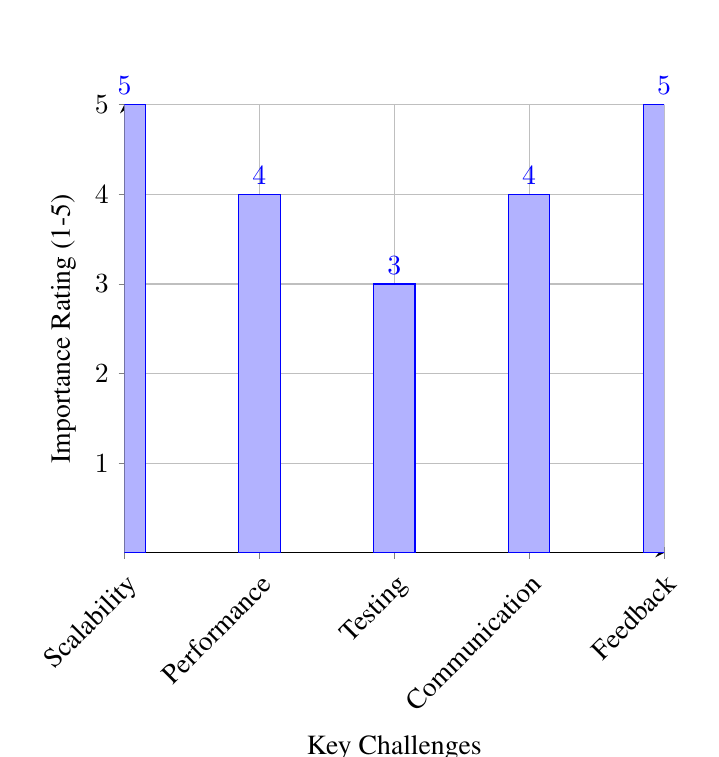
\begin{tikzpicture}
        \begin{axis}[
            ybar,
            symbolic x coords={Scalability, Performance, Testing, Communication, Feedback},
            xtick=data,
            ylabel={Importance Rating (1-5)},
            xlabel={Key Challenges},
            title={},
            bar width=15pt,
            enlarge x limits=0.4,
            ymin=0, ymax=5,
            nodes near coords,
            grid=major,
            ytick={1,2,3,4,5},
            axis x line=bottom,
            axis y line=left,
            every axis label/.append style={font=\normalsize},
            every axis tick/.append style={font=\small},
            xticklabel style={rotate=45, anchor=north east}, % Rotates x-axis labels to prevent overlap
            title style={yshift=-1ex} % Shifts the title slightly down to avoid overlap
        ]
            \addplot coordinates {(Scalability, 5) (Performance, 4) (Testing, 3) (Communication, 4) (Feedback, 5)};
        \end{axis}
    \end{tikzpicture}
    \caption{Employee Ranking of Key Challenges.}
    \label{fig:employee_challenges}
\end{figure}

\textbf{Key Findings:} The employee ranking data reveals that scalability and feedback mechanisms are perceived as the most critical challenges, both receiving the maximum rating of 5. Performance optimization and communication issues follow closely with a rating of 4, while testing processes are viewed as moderately challenging with a rating of 3. This prioritization indicates that employees recognize the urgent need for addressing scalability limitations and establishing robust feedback systems to support the platform's growth trajectory.

\begin{figure}[H]
    \centering
    \includegraphics[width=1.0\textwidth]{Screenshot 2025-07-26 at 1.32.02 AM.png} % Change the filename here
    \caption{Employee Responses: Technical Debt Impact Assessment}
    \label{fig:technical_debt_impact}
\end{figure}

\textbf{Key Findings:} The technical debt impact assessment demonstrates a significant correlation between accumulated technical debt and decreased system performance. The data shows that areas with higher technical debt concentrations experience more frequent bottlenecks and require additional maintenance overhead. This finding reinforces the need for systematic refactoring initiatives and suggests that investment in code quality improvements will yield substantial returns in platform stability and development velocity.

\begin{figure}[H]
    \centering
    \includegraphics[width=1.0\textwidth]{Screenshot 2025-07-26 at 1.26.05 AM.png} % Change the filename here
    \caption{Employee Responses: Cross-Team Communication Challenges}
    \label{fig:communication_challenges}
\end{figure}

\textbf{Key Findings:} The cross-team communication analysis reveals significant gaps in information flow between different departments, particularly between technical and academic teams. The data indicates that communication breakdowns occur most frequently during project transitions and deadline-critical phases. These findings suggest that implementing structured communication protocols and establishing clear escalation pathways could substantially improve coordination efficiency and reduce project delivery delays.

\begin{figure}[h!]
    \centering
    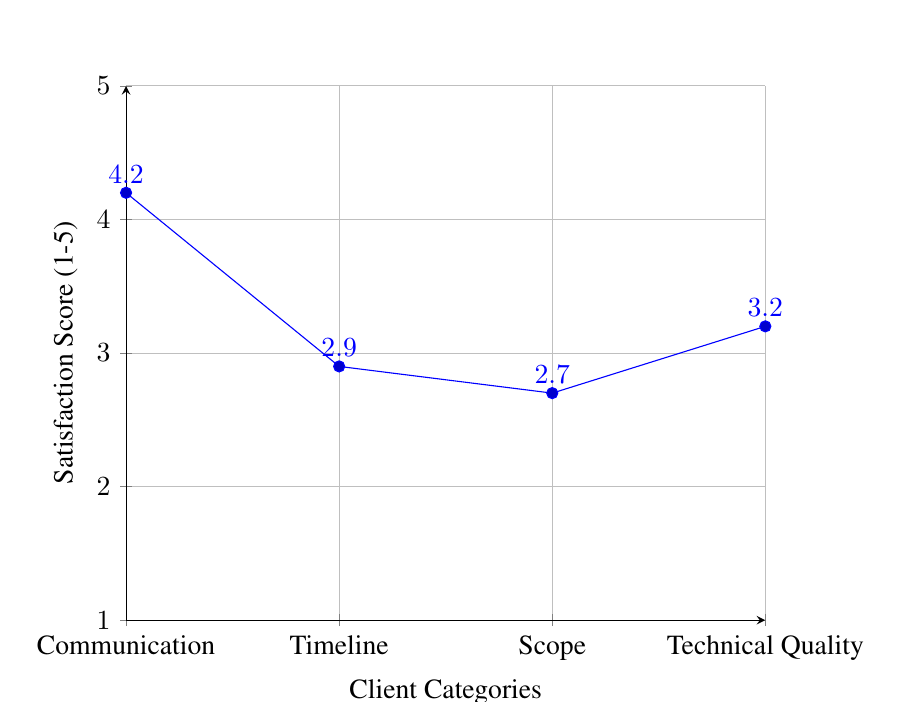
\begin{tikzpicture}
        \begin{axis}[
            width=0.8\textwidth,
            symbolic x coords={Communication, Timeline, Scope, Technical Quality},
            xtick=data,
            ylabel={Satisfaction Score (1-5)},
            xlabel={Client Categories},
            title={},
            bar width=15pt,
            enlarge x limits=0.4,
            ymin=1, ymax=5,
            nodes near coords,
            grid=major,
            ytick={1,2,3,4,5},
            axis x line=bottom,
            axis y line=left,
            every axis label/.append style={font=\normalsize},
            every axis tick/.append style={font=\small}
        ]
            \addplot coordinates {(Communication, 4.2) (Timeline, 2.9) (Scope, 2.7) (Technical Quality, 3.2)};
        \end{axis}
    \end{tikzpicture}
    \caption{Client Satisfaction Ratings for Service Aspects.}
    \label{fig:client_service_ratings}
\end{figure}

\textbf{Key Findings:} Client satisfaction data reveals a notable disparity across service delivery aspects. Communication receives the highest satisfaction rating at 4.2, indicating effective client relationship management. However, critical areas show concerning performance: timeline adherence (2.9) and scope management (2.7) fall significantly below acceptable thresholds. Technical quality receives a moderate rating of 3.2, suggesting room for improvement. These findings highlight the urgent need for enhanced project management methodologies and scope control mechanisms to align client expectations with delivery capabilities.

% Adding a more advanced bar chart with multiple series (data comparison)






\newpage

\begin{figure}[H]
    \centering
    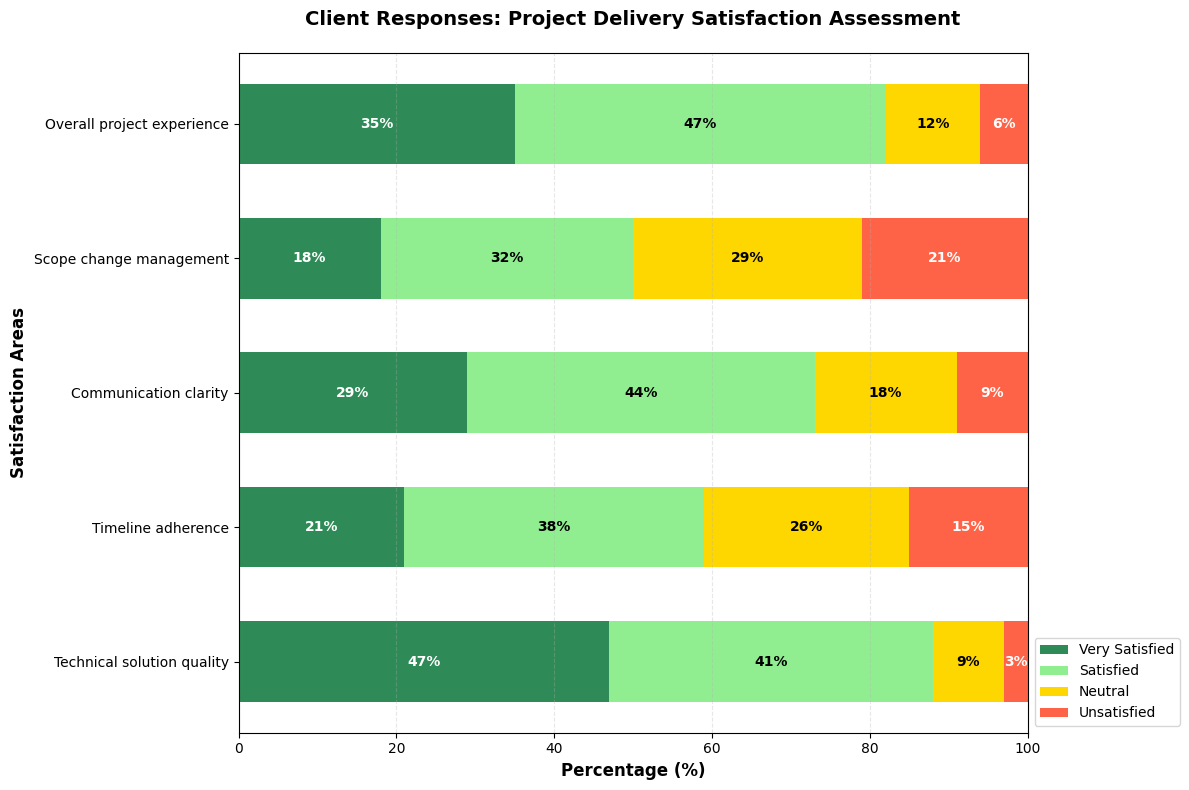
\includegraphics[width=1.0\textwidth]{download.png} % Change the filename here
    \caption{Client Responses: Project Delivery Satisfaction Assessment}
    \label{fig:client_satisfaction}
\end{figure}

\textbf{Key Findings:} The project delivery satisfaction assessment provides comprehensive insights into client experience across multiple dimensions. The analysis shows that while initial project engagement and requirement gathering phases receive positive feedback, mid-project communication and timeline management present significant challenges. Clients consistently report satisfaction with final deliverable quality but express concerns about predictability and transparency during development phases. These findings emphasize the importance of implementing robust project tracking systems and maintaining regular client touchpoints throughout the development lifecycle.
\newpage
\subsection{Data Flow Diagrams (DFD) of Existing System}

Data Flow Diagrams provide a graphical representation of how data moves through Chorcha's existing information system. This analysis examines the current system architecture, data flows, and processing mechanisms to identify bottlenecks and areas for improvement. The DFD analysis is structured in hierarchical levels, starting from the context diagram (Level 0) and decomposing into detailed process flows.

\subsubsection{Context Diagram (Level 0 DFD)}

The context diagram presents the highest-level view of Chorcha's system, showing the major external entities that interact with the platform and the primary data flows between them.

\begin{figure}[H]
    \centering
    \scalebox{0.6}{%
    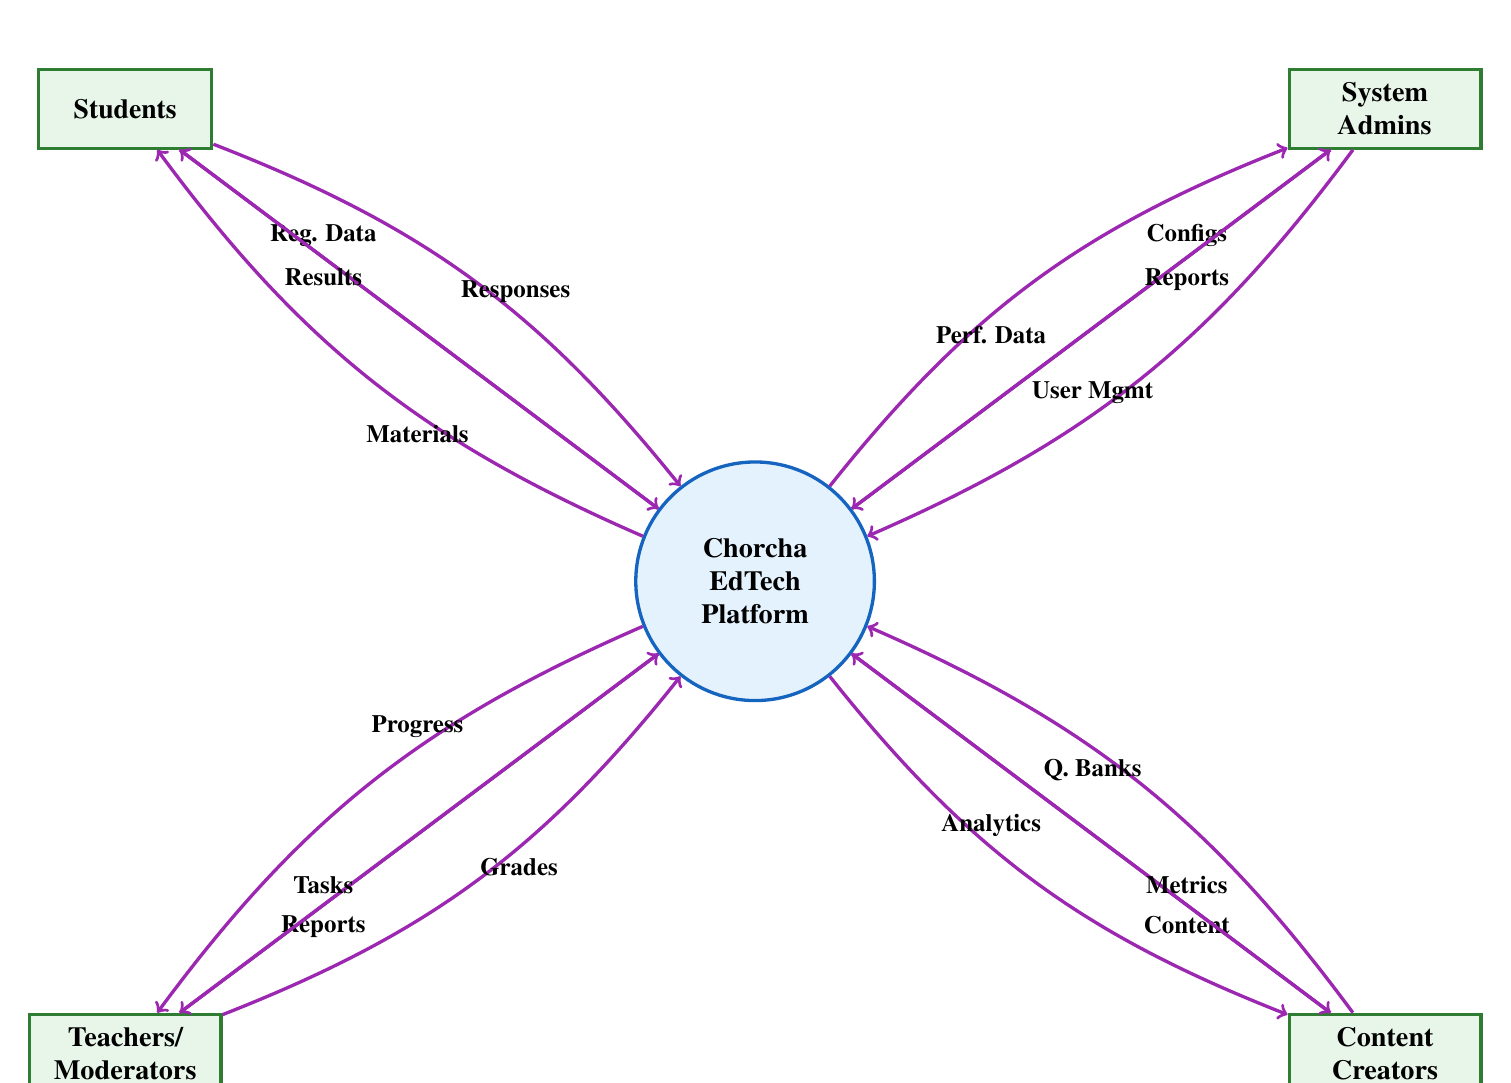
\begin{tikzpicture}[
        node distance=3cm,
        entity/.style={rectangle, draw=entitygreen, very thick, minimum width=2.2cm, minimum height=1cm, fill=lightgreen, text=textblack},
        process/.style={circle, draw=processblue, very thick, minimum size=2.8cm, fill=lightblue, text=textblack},
        datastore/.style={rectangle, draw=datastoreorange, very thick, minimum width=2.2cm, minimum height=0.6cm, fill=lightorange, text=textblack},
        flow/.style={->, very thick, color=flowpurple}
    ]
    
    % External Entities arranged for portrait orientation
    \node[entity] (student) at (-8, 6) {\textbf{Students}};
    \node[entity, text width=2.2cm, align=center] (teacher) at (-8, -6) {\textbf{Teachers/\\ Moderators}};
    \node[entity, text width=2.2cm, align=center] (admin) at (8, 6) {\textbf{System\\ Admins}};
    \node[entity, text width=2.2cm, align=center] (content) at (8, -6) {\textbf{Content\\ Creators}};
    
    % Main Process in center
    \node[process, text width=2.5cm, align=center] (system) at (0, 0) {\textbf{Chorcha\\ EdTech\\ Platform}};
    
    % Data Flows - Students (with shorter labels)
    \draw[flow] (student) -- node[above, pos=0.3] {\small\textbf{\textcolor{black}{Reg. Data}}} (system);
    \draw[flow] (system) -- node[below, pos=0.7] {\small\textbf{\textcolor{black}{Results}}} (student);
    \draw[flow] (student) to[bend left=15] node[above, pos=0.6] {\small\textbf{\textcolor{black}{Responses}}} (system);
    \draw[flow] (system) to[bend left=15] node[below, pos=0.4] {\small\textbf{\textcolor{black}{Materials}}} (student);
    
    % Data Flows - Teachers (with shorter labels)
    \draw[flow] (teacher) -- node[below, pos=0.3] {\small\textbf{\textcolor{black}{Reports}}} (system);
    \draw[flow] (system) -- node[above, pos=0.7] {\small\textbf{\textcolor{black}{Tasks}}} (teacher);
    \draw[flow] (teacher) to[bend right=15] node[below, pos=0.6] {\small\textbf{\textcolor{black}{Grades}}} (system);
    \draw[flow] (system) to[bend right=15] node[above, pos=0.4] {\small\textbf{\textcolor{black}{Progress}}} (teacher);
    
    % Data Flows - Administrators (with shorter labels)
    \draw[flow] (admin) -- node[above, pos=0.3] {\small\textbf{\textcolor{black}{Configs}}} (system);
    \draw[flow] (system) -- node[below, pos=0.7] {\small\textbf{\textcolor{black}{Reports}}} (admin);
    \draw[flow] (admin) to[bend left=15] node[above, pos=0.6] {\small\textbf{\textcolor{black}{User Mgmt}}} (system);
    \draw[flow] (system) to[bend left=15] node[below, pos=0.4] {\small\textbf{\textcolor{black}{Perf. Data}}} (admin);
    
    % Data Flows - Content Creators (with shorter labels)
    \draw[flow] (content) -- node[below, pos=0.3] {\small\textbf{\textcolor{black}{Content}}} (system);
    \draw[flow] (system) -- node[above, pos=0.7] {\small\textbf{\textcolor{black}{Metrics}}} (content);
    \draw[flow] (content) to[bend right=15] node[below, pos=0.6] {\small\textbf{\textcolor{black}{Q. Banks}}} (system);
    \draw[flow] (system) to[bend right=15] node[above, pos=0.4] {\small\textbf{\textcolor{black}{Analytics}}} (content);
    
    \end{tikzpicture}
    }% End scalebox
    \caption{Context Diagram - Chorcha EdTech Platform (Level 0 DFD)}
\end{figure}

\textbf{Context Diagram Analysis:}

The context diagram reveals four primary external entities interacting with Chorcha's system:

\textbf{Students} represent the primary users who register, take exams, submit responses, and receive study materials and results. The bidirectional data flow indicates both input (registration, responses) and output (materials, results) interactions.

\vspace{0.3cm}
\textbf{Teachers/Moderators} are responsible for content quality control, manual evaluation of subjective responses, and question report verification. They receive evaluation tasks from the system and provide manual grades and quality feedback.

\vspace{0.3cm}
\textbf{System Administrators} manage platform configuration, user accounts, and monitor system performance. They input system configurations and user management data while receiving performance reports and system analytics.

\vspace{0.3cm}
\textbf{Content Creators} develop and maintain the question banks, study materials, and assessment content. They contribute new content and question sets while receiving usage analytics and content performance metrics.

\subsubsection{Level 1 DFD - Main System Processes}

The Level 1 DFD decomposes the main system into core functional processes, showing detailed data flows between processes and data stores.

\begin{figure}[H]
    \centering
    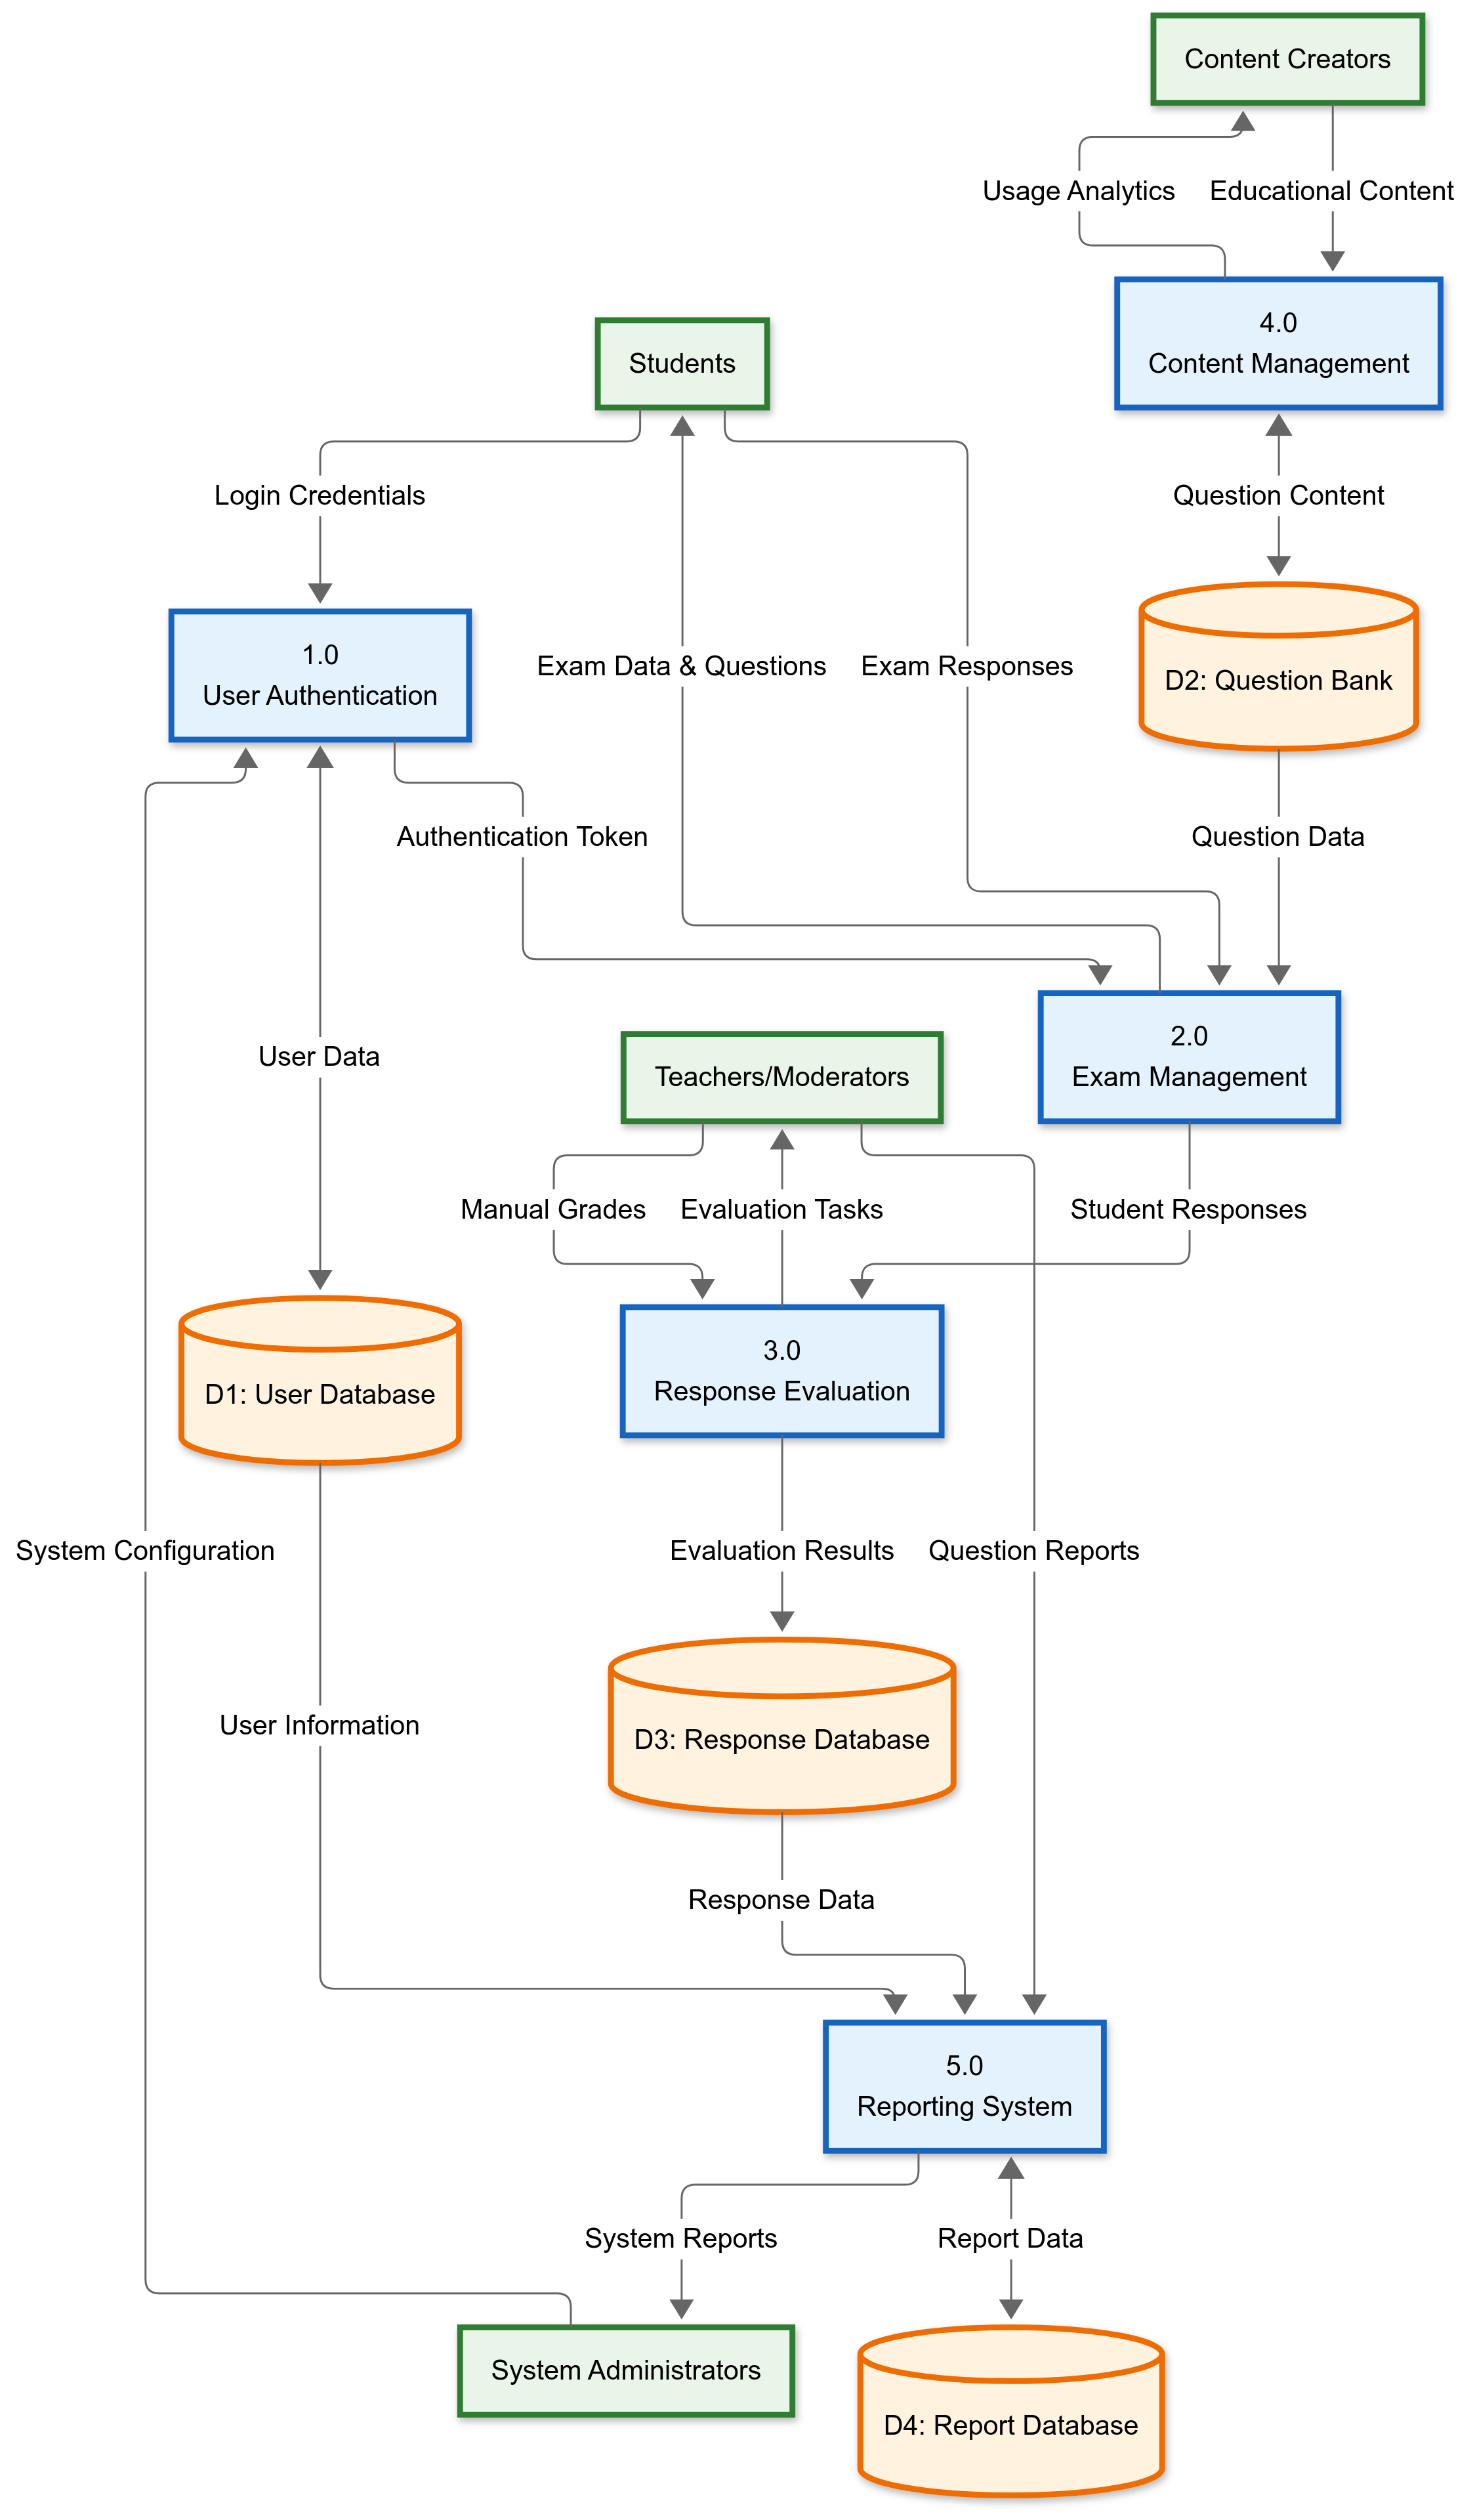
\includegraphics[width=0.7\textwidth]{Level1DFD.png}
    \caption{Level 1 DFD - Main System Processes}
\end{figure}

\textbf{Level 1 DFD Process Analysis:}

\textbf{Process 1.0 - User Authentication:} Handles user login, registration, and session management. Interacts with the User Database (D1) to verify credentials and maintain user sessions. This process is critical for security but currently shows bottlenecks during peak login times.

\vspace{0.3cm}
\textbf{Process 2.0 - Exam Management:} Manages exam delivery, question presentation, and response collection. Retrieves questions from the Question Bank (D2) and forwards student responses to the evaluation process. Performance issues are evident during high-traffic exam periods.

\vspace{0.3cm}
\textbf{Process 3.0 - Response Evaluation:} Handles both automated and manual evaluation of student responses. For subjective questions, this process creates evaluation tasks for teachers and processes their manual grades. The manual component creates scalability challenges.

\vspace{0.3cm}
\textbf{Process 4.0 - Content Management:} Manages the creation, update, and organization of educational content and question banks. Content creators input new materials, which are processed and stored in the Question Bank (D2).

\vspace{0.3cm}
\textbf{Process 5.0 - Reporting System:} Generates various reports for administrators, teachers, and students. Aggregates data from multiple sources including response data, user activity, and system performance metrics.

\vspace{0.5cm}
\textbf{Data Store Analysis:}

\textbf{D1 - User Database:} Stores user profiles, authentication data, and session information. Currently experiencing performance issues due to lack of indexing optimization.

\vspace{0.3cm}
\textbf{D2 - Question Bank:} Contains all educational content, questions, and metadata. The large volume of data and frequent access patterns create retrieval bottlenecks.

\vspace{0.3cm}
\textbf{D3 - Response Database:} Stores student responses, evaluation results, and progress tracking data. Rapid growth in data volume affects query performance.

\vspace{0.3cm}
\textbf{D4 - Report Database:} Contains aggregated data for reporting and analytics. Manual report generation processes create delays in data availability.

\vspace{0.5cm}
\textbf{Critical Data Flow Issues Identified:}

1. \textbf{Manual Evaluation Bottleneck:} The flow from Process 3.0 to teachers for manual evaluation creates significant delays in feedback delivery.

\vspace{0.3cm}
2. \textbf{Peak Load Vulnerabilities:} Authentication and exam management processes show strain during simultaneous user access.

\vspace{0.3cm}
3. \textbf{Report Generation Delays:} Manual aggregation in the reporting system causes delayed insights for stakeholders.

\vspace{0.3cm}
4. \textbf{Data Store Performance:} All major data stores exhibit performance degradation under high load conditions.

\vspace{0.5cm}
These DFD analyses reveal that while Chorcha's existing system architecture provides comprehensive functionality, several critical bottlenecks limit scalability and performance. The manual evaluation process, peak load vulnerabilities, and data store performance issues directly correlate with the problems identified in earlier chapters, providing a clear technical foundation for the proposed solutions in the feasibility study.

\vspace{0.5cm}
\newpage
\subsubsection{Problem-Specific Data Flow Diagrams}

The following DFD diagrams illustrate the specific data flow issues and bottlenecks identified in Chorcha's current system. Each diagram focuses on a particular problem area to provide detailed insight into the root causes and potential solutions.

\vspace{0.3cm}

\textbf{Problem 1: Manual Evaluation Bottleneck DFD}

\begin{figure}[H]
    \centering
    \scalebox{0.8}{%
    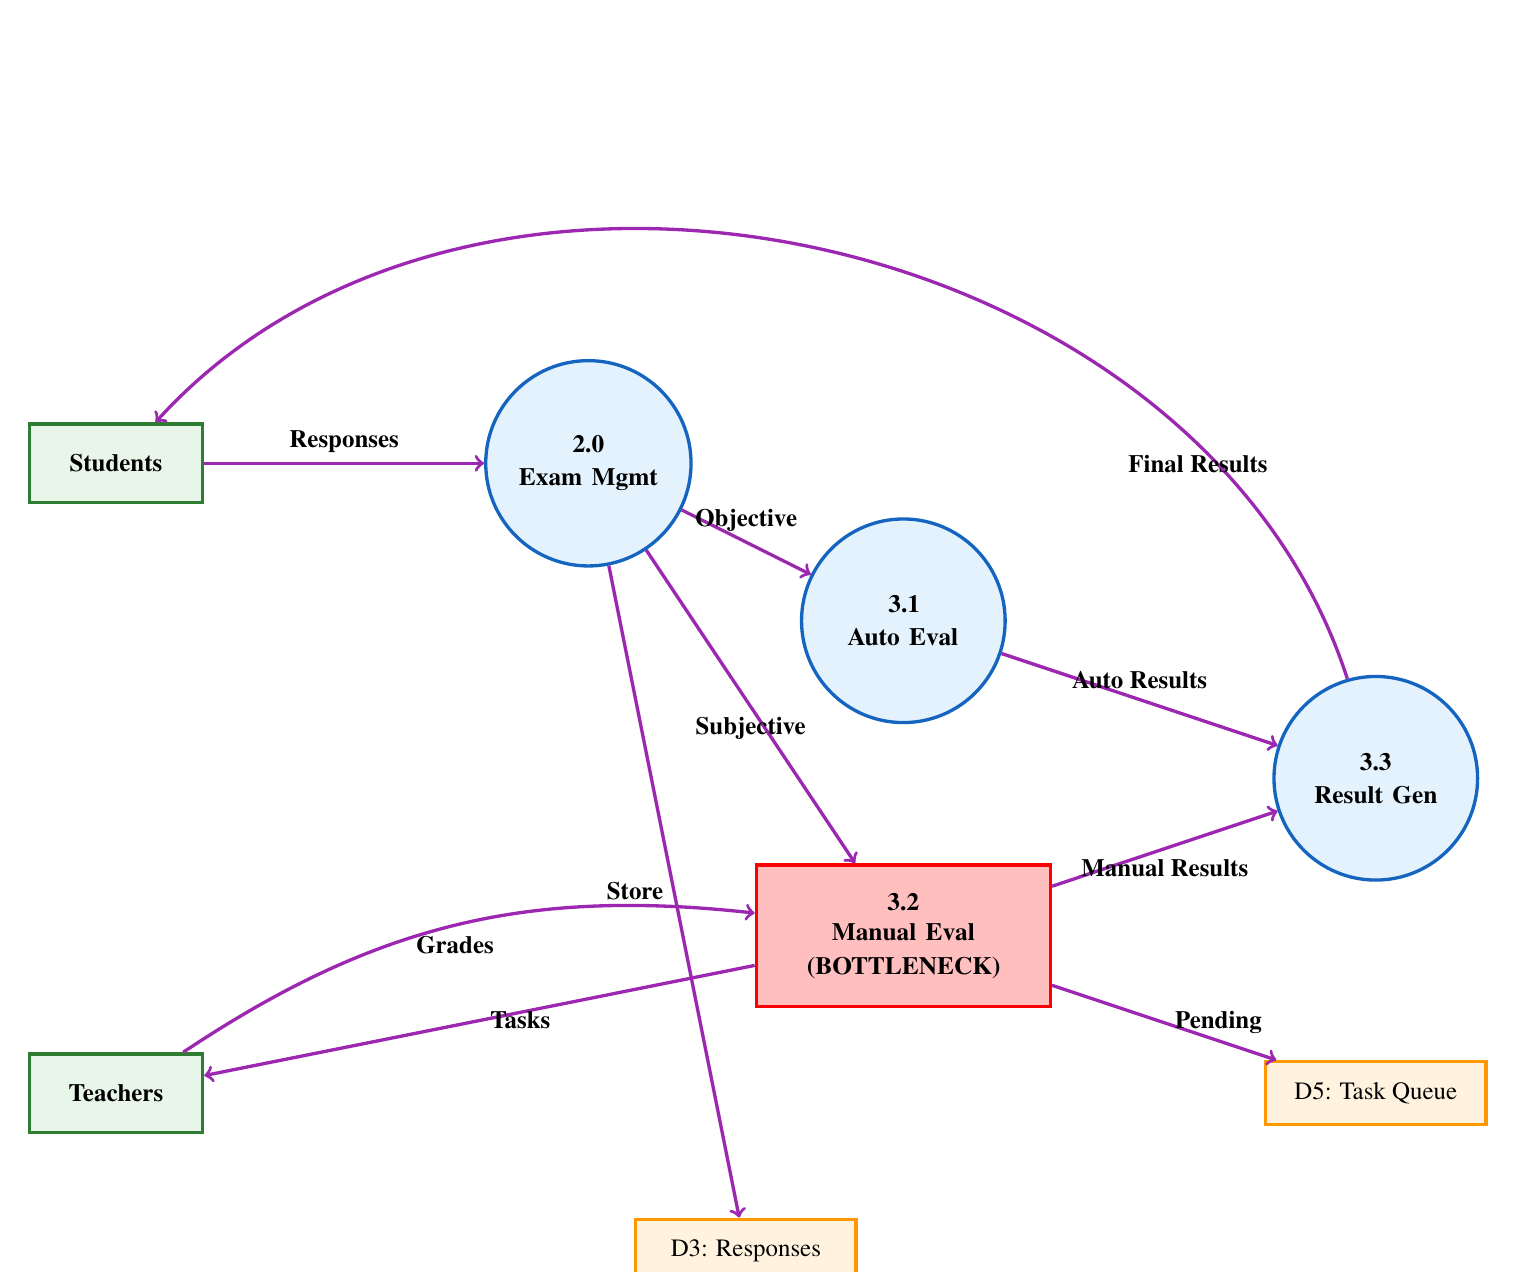
\begin{tikzpicture}[
        node distance=3cm,
        entity/.style={rectangle, draw=entitygreen, very thick, minimum width=2.2cm, minimum height=1cm, fill=lightgreen, text=textblack},
        process/.style={circle, draw=processblue, very thick, minimum size=2.5cm, fill=lightblue, text=textblack},
        datastore/.style={rectangle, draw=datastoreorange, very thick, minimum width=2.8cm, minimum height=0.8cm, fill=lightorange, text=textblack},
        flow/.style={->, very thick, color=flowpurple},
        bottleneck/.style={rectangle, draw=red, very thick, minimum width=2.5cm, minimum height=1.2cm, fill=pink, text=textblack}
    ]
    
    % Entities
    \node[entity] (student) at (-8, 4) {\small\textbf{Students}};
    \node[entity] (teacher) at (-8, -4) {\small\textbf{Teachers}};
    
    % Main Processes
    \node[process, text width=2.2cm, align=center] (exam) at (-2, 4) {\small\textbf{2.0\\ Exam Mgmt}};
    \node[process, text width=2.2cm, align=center] (auto_eval) at (2, 2) {\small\textbf{3.1\\ Auto Eval}};
    \node[bottleneck, text width=3.5cm, minimum height=1.8cm, align=center] (manual_eval) at (2, -2) {\small\textbf{3.2\\ Manual Eval\\ (BOTTLENECK)}};
    \node[process, text width=2.2cm, align=center] (result_gen) at (8, 0) {\small\textbf{3.3\\ Result Gen}};
    
    % Data Stores
    \node[datastore] (responsedb) at (0, -6) {\small D3: Responses};
    \node[datastore] (taskqueue) at (8, -4) {\small D5: Task Queue};
    
    % Data Flows
    \draw[flow] (student) -- node[above, pos=0.5] {\small\textbf{\textcolor{black}{Responses}}} (exam);
    \draw[flow] (exam) -- node[above, pos=0.5] {\small\textbf{\textcolor{black}{Objective}}} (auto_eval);
    \draw[flow] (exam) -- node[below, pos=0.5] {\small\textbf{\textcolor{black}{Subjective}}} (manual_eval);
    \draw[flow] (auto_eval) -- node[above, pos=0.5] {\small\textbf{\textcolor{black}{Auto Results}}} (result_gen);
    \draw[flow] (manual_eval) -- node[below, pos=0.5] {\small\textbf{\textcolor{black}{Manual Results}}} (result_gen);
    \draw[flow] (manual_eval) -- node[right, pos=0.5] {\small\textbf{\textcolor{black}{Tasks}}} (teacher);
    \draw[flow] (teacher) to[bend left=20] node[below, pos=0.5] {\small\textbf{\textcolor{black}{Grades}}} (manual_eval);
    \draw[flow] (manual_eval) -- node[right, pos=0.5] {\small\textbf{\textcolor{black}{Pending}}} (taskqueue);
    \draw[flow] (exam) -- node[left, pos=0.5] {\small\textbf{\textcolor{black}{Store}}} (responsedb);
    \draw[flow] (result_gen) to[bend right=60] node[below, pos=0.2] {\small\textbf{\textcolor{black}{Final Results}}} (student);
    
    \end{tikzpicture}
    }
    \caption{Problem 1: Manual Evaluation Bottleneck DFD}
\end{figure}

\textbf{DFD Description:} 
\begin{itemize}
    \item Students submit responses that are split into objective and subjective categories
    \item Objective questions are automatically evaluated through the Auto Eval process (3.1)
    \item Subjective questions require manual evaluation, creating a bottleneck at process 3.2
    \item Manual evaluation tasks are queued and assigned to teachers
    \item Teachers must manually grade subjective responses before results can be generated
    \item The bottleneck grows during peak exam periods when teacher availability is limited
    \item Delayed manual evaluation causes overall result delivery delays to students
\end{itemize}

\vspace{0.5cm}

\textbf{Problem 2: Peak Load Authentication Vulnerabilities DFD}

\begin{figure}[H]
    \centering
    \scalebox{0.8}{%
    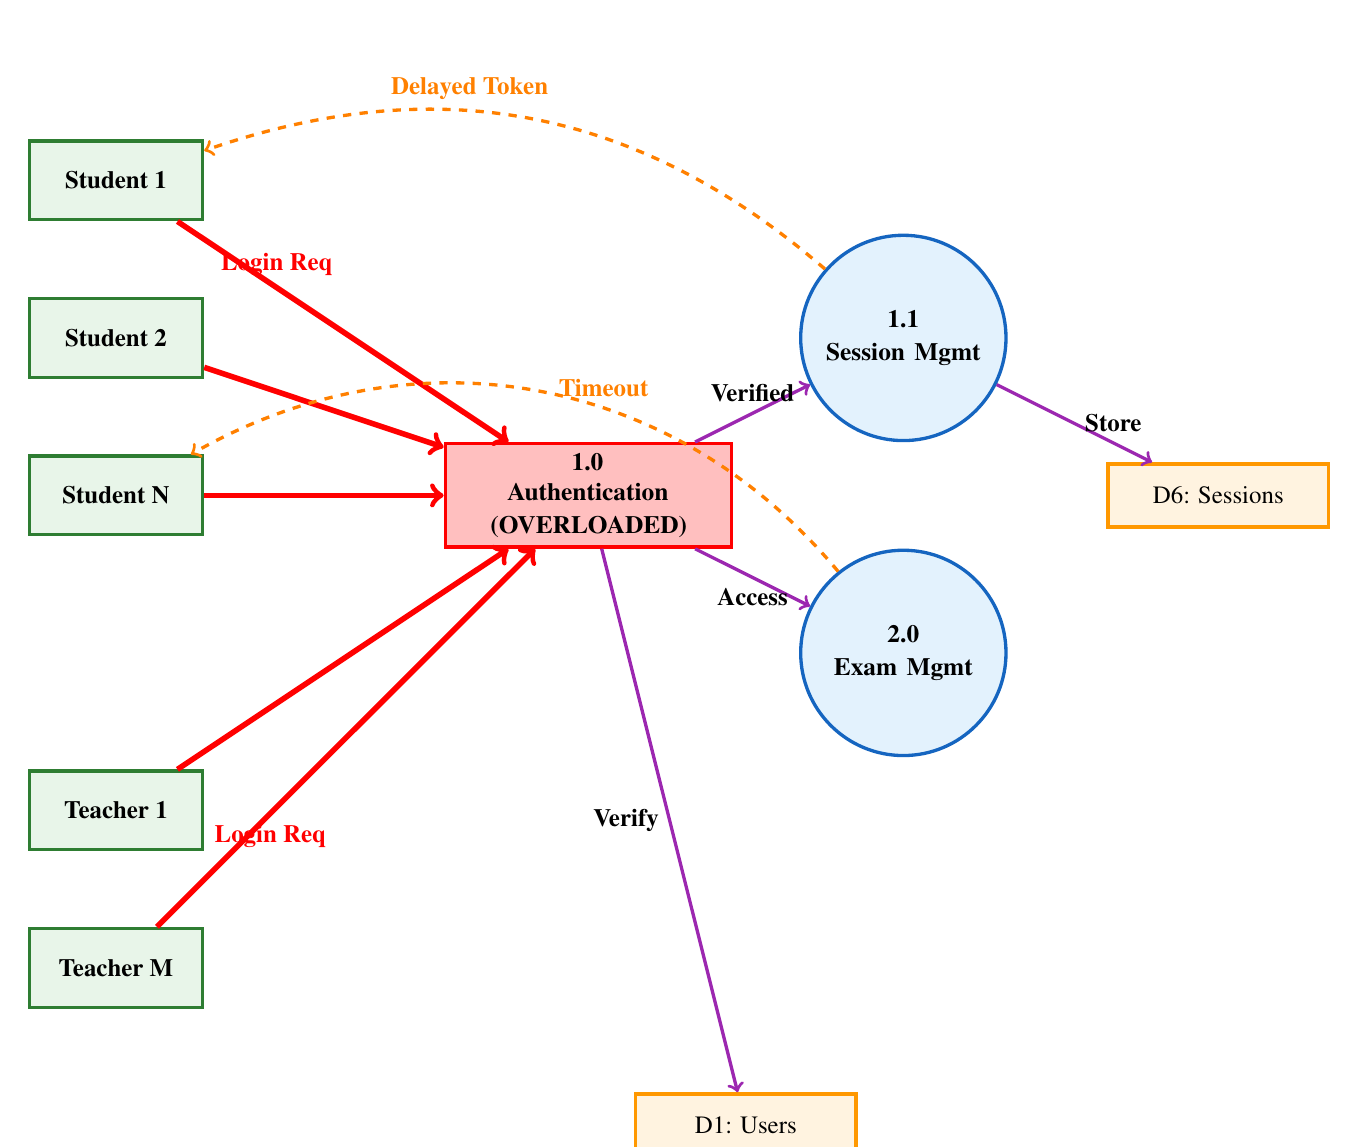
\begin{tikzpicture}[
        node distance=3cm,
        entity/.style={rectangle, draw=entitygreen, very thick, minimum width=2.2cm, minimum height=1cm, fill=lightgreen, text=textblack},
        process/.style={circle, draw=processblue, very thick, minimum size=2.5cm, fill=lightblue, text=textblack},
        datastore/.style={rectangle, draw=datastoreorange, very thick, minimum width=2.8cm, minimum height=0.8cm, fill=lightorange, text=textblack},
        flow/.style={->, very thick, color=flowpurple},
        bottleneck/.style={rectangle, draw=red, very thick, minimum width=2.5cm, minimum height=1.2cm, fill=pink, text=textblack}
    ]
    
    % Multiple Users
    \node[entity] (student1) at (-8, 6) {\small\textbf{Student 1}};
    \node[entity] (student2) at (-8, 4) {\small\textbf{Student 2}};
    \node[entity] (student3) at (-8, 2) {\small\textbf{Student N}};
    \node[entity] (teacher1) at (-8, -2) {\small\textbf{Teacher 1}};
    \node[entity] (teacher2) at (-8, -4) {\small\textbf{Teacher M}};
    
    % Authentication Process (Bottleneck)
    \node[bottleneck, text width=3.4cm, align=center] (auth) at (-2, 2) {\small\textbf{1.0\\ Authentication\\ (OVERLOADED)}};
    \node[process, text width=2.2cm, align=center] (session) at (2, 4) {\small\textbf{1.1\\ Session Mgmt}};
    \node[process, text width=2.2cm, align=center] (exam) at (2, 0) {\small\textbf{2.0\\ Exam Mgmt}};
    
    % Data Stores
    \node[datastore] (userdb) at (0, -6) {\small D1: Users};
    \node[datastore] (sessiondb) at (6, 2) {\small D6: Sessions};
    
    % Congested Flows
    \draw[flow, line width=2pt, color=red] (student1) -- node[above, pos=0.3] {\small\textbf{\textcolor{red}{Login Req}}} (auth);
    \draw[flow, line width=2pt, color=red] (student2) -- (auth);
    \draw[flow, line width=2pt, color=red] (student3) -- (auth);
    \draw[flow, line width=2pt, color=red] (teacher1) -- (auth);
    \draw[flow, line width=2pt, color=red] (teacher2) -- node[below, pos=0.3] {\small\textbf{\textcolor{red}{Login Req}}} (auth);
    
    % Normal Flows
    \draw[flow] (auth) -- node[above, pos=0.5] {\small\textbf{\textcolor{black}{Verified}}} (session);
    \draw[flow] (session) -- node[right, pos=0.5] {\small\textbf{\textcolor{black}{Store}}} (sessiondb);
    \draw[flow] (auth) -- node[below, pos=0.5] {\small\textbf{\textcolor{black}{Access}}} (exam);
    \draw[flow] (auth) -- node[left, pos=0.5] {\small\textbf{\textcolor{black}{Verify}}} (userdb);
    
    % Delayed Responses
    \draw[flow, dashed, color=orange] (session) to[bend right=30] node[above, pos=0.6] {\small\textbf{\textcolor{orange}{Delayed Token}}} (student1);
    \draw[flow, dashed, color=orange] (exam) to[bend right=40] node[above, pos=0.4] {\small\textbf{\textcolor{orange}{Timeout}}} (student3);
    
    \end{tikzpicture}
    }
    \caption{Problem 2: Peak Load Authentication Vulnerabilities DFD}
\end{figure}

\textbf{DFD Description:} 
\begin{itemize}
    \item Multiple students and teachers attempt simultaneous login during peak exam periods
    \item All login requests converge on the single Authentication process (1.0)
    \item The authentication system becomes overloaded with concurrent requests
    \item Database verification queries create additional bottlenecks
    \item Login failures and timeouts occur due to system overload
    \item Users repeatedly retry failed logins, further increasing system load
    \item Session management and exam access are delayed or blocked
    \item The cascading effect prevents legitimate users from accessing the platform
\end{itemize}

\vspace{0.5cm}
\newpage
\textbf{Problem 3: Report Generation Delays DFD}

\begin{figure}[H]
    \centering
    \scalebox{0.8}{%
    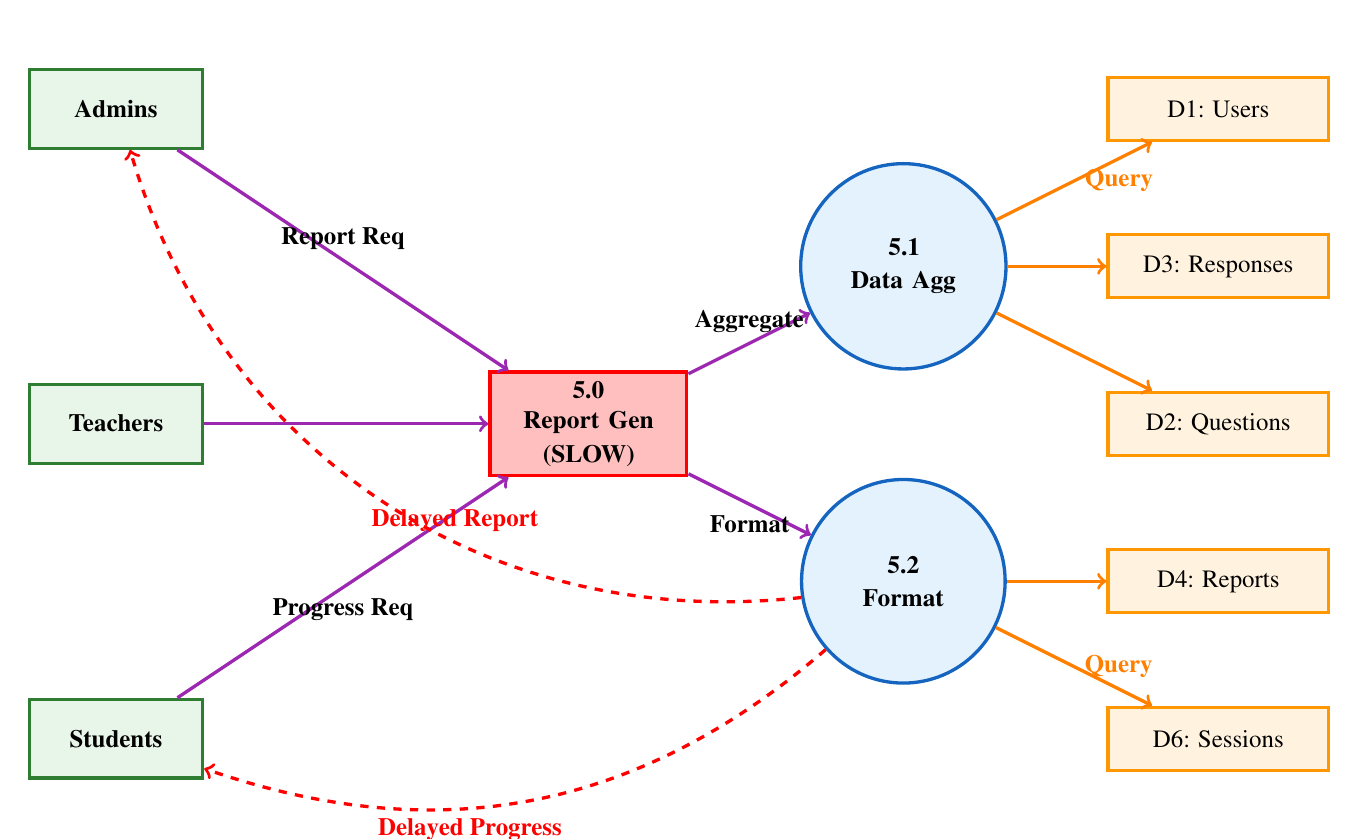
\begin{tikzpicture}[
        node distance=3cm,
        entity/.style={rectangle, draw=entitygreen, very thick, minimum width=2.2cm, minimum height=1cm, fill=lightgreen, text=textblack},
        process/.style={circle, draw=processblue, very thick, minimum size=2.5cm, fill=lightblue, text=textblack},
        datastore/.style={rectangle, draw=datastoreorange, very thick, minimum width=2.8cm, minimum height=0.8cm, fill=lightorange, text=textblack},
        flow/.style={->, very thick, color=flowpurple},
        bottleneck/.style={rectangle, draw=red, very thick, minimum width=2.5cm, minimum height=1.2cm, fill=pink, text=textblack}
    ]
    
    % Entities
    \node[entity] (admin) at (-8, 4) {\small\textbf{Admins}};
    \node[entity] (teacher) at (-8, 0) {\small\textbf{Teachers}};
    \node[entity] (student) at (-8, -4) {\small\textbf{Students}};
    
    % Report Generation Process (Bottleneck)
    \node[bottleneck, text width=2.2cm, align=center] (report_gen) at (-2, 0) {\small\textbf{5.0\\ Report Gen\\ (SLOW)}};
    \node[process, text width=2.2cm, align=center] (data_agg) at (2, 2) {\small\textbf{5.1\\ Data Agg}};
    \node[process, text width=2.2cm, align=center] (format) at (2, -2) {\small\textbf{5.2\\ Format}};
    
    % Multiple Data Sources
    \node[datastore] (userdb) at (6, 4) {\small D1: Users};
    \node[datastore] (responsedb) at (6, 2) {\small D3: Responses};
    \node[datastore] (questiondb) at (6, 0) {\small D2: Questions};
    \node[datastore] (reportdb) at (6, -2) {\small D4: Reports};
    \node[datastore] (sessiondb) at (6, -4) {\small D6: Sessions};
    
    % Request Flows
    \draw[flow] (admin) -- node[above, pos=0.5] {\small\textbf{\textcolor{black}{Report Req}}} (report_gen);
    \draw[flow] (teacher) -- (report_gen);
    \draw[flow] (student) -- node[below, pos=0.5] {\small\textbf{\textcolor{black}{Progress Req}}} (report_gen);
    
    % Processing Flows
    \draw[flow] (report_gen) -- node[above, pos=0.5] {\small\textbf{\textcolor{black}{Aggregate}}} (data_agg);
    \draw[flow] (report_gen) -- node[below, pos=0.5] {\small\textbf{\textcolor{black}{Format}}} (format);
    
    % Data Access (Multiple sources causing delays)
    \draw[flow, color=orange] (data_agg) -- node[right, pos=0.5] {\small\textbf{\textcolor{orange}{Query}}} (userdb);
    \draw[flow, color=orange] (data_agg) -- (responsedb);
    \draw[flow, color=orange] (data_agg) -- (questiondb);
    \draw[flow, color=orange] (format) -- (reportdb);
    \draw[flow, color=orange] (format) -- node[right, pos=0.5] {\small\textbf{\textcolor{orange}{Query}}} (sessiondb);
    
    % Delayed Output
    \draw[flow, dashed, color=red] (format) to[bend left=40] node[above, pos=0.4] {\small\textbf{\textcolor{red}{Delayed Report}}} (admin);
    \draw[flow, dashed, color=red] (format) to[bend left=30] node[below, pos=0.6] {\small\textbf{\textcolor{red}{Delayed Progress}}} (student);
    
    \end{tikzpicture}
    }
    \caption{Problem 3: Report Generation Delays DFD}
\end{figure}

\textbf{DFD Description:} 
\begin{itemize}
    \item Administrators, teachers, and students request various types of reports
    \item All requests flow through the central Report Generation process (5.0)
    \item Data Aggregation process (5.1) must query multiple data sources simultaneously
    \item The system accesses Users, Responses, Questions, Reports, and Sessions databases
    \item Manual data aggregation creates processing delays
    \item Format process (5.2) must combine and structure data from multiple sources
    \item Complex database queries and joins slow down the entire process
    \item Reports are delivered with significant delays, affecting decision-making
\end{itemize}

\vspace{0.5cm}
\newpage
\textbf{Problem 4: Data Store Performance Degradation DFD}

\begin{figure}[H]
    \centering
    \scalebox{0.8}{%
    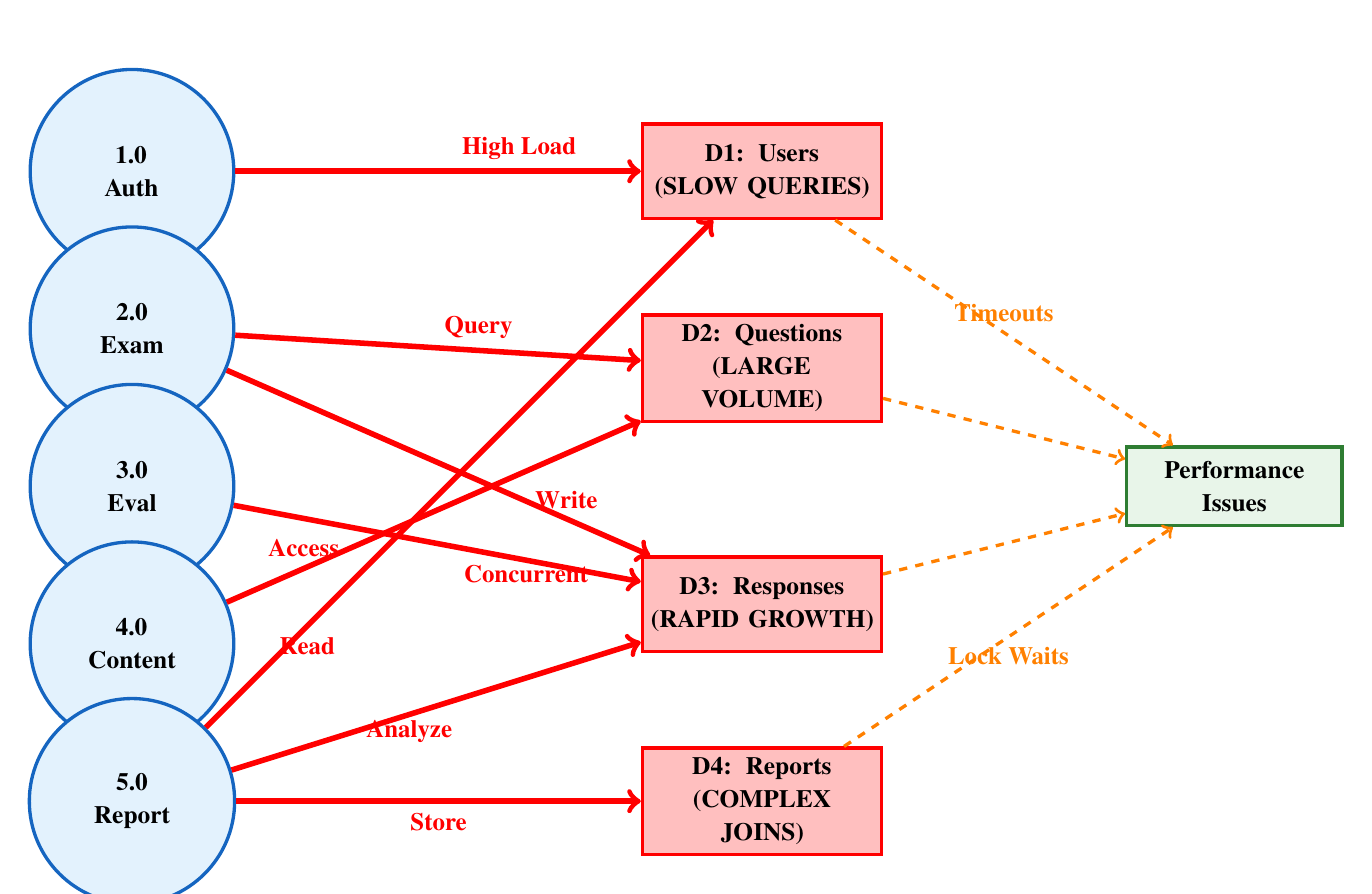
\begin{tikzpicture}[
        node distance=3cm,
        entity/.style={rectangle, draw=entitygreen, very thick, minimum width=2.2cm, minimum height=1cm, fill=lightgreen, text=textblack},
        process/.style={circle, draw=processblue, very thick, minimum size=2.5cm, fill=lightblue, text=textblack},
        datastore/.style={rectangle, draw=datastoreorange, very thick, minimum width=2.8cm, minimum height=0.8cm, fill=lightorange, text=textblack},
        flow/.style={->, very thick, color=flowpurple},
        bottleneck/.style={rectangle, draw=red, very thick, minimum width=2.5cm, minimum height=1.2cm, fill=pink, text=textblack}
    ]
    
    % Processes accessing databases
    \node[process, text width=2.2cm, align=center] (auth) at (-6, 4) {\small\textbf{1.0\\ Auth}};
    \node[process, text width=2.2cm, align=center] (exam) at (-6, 2) {\small\textbf{2.0\\ Exam}};
    \node[process, text width=2.2cm, align=center] (eval) at (-6, 0) {\small\textbf{3.0\\ Eval}};
    \node[process, text width=2.2cm, align=center] (content) at (-6, -2) {\small\textbf{4.0\\ Content}};
    \node[process, text width=2.2cm, align=center] (report) at (-6, -4) {\small\textbf{5.0\\ Report}};
    
    % Bottleneck Data Stores
    \node[bottleneck, text width=2.8cm, align=center] (userdb) at (2, 4) {\small\textbf{D1: Users\\ (SLOW QUERIES)}};
    \node[bottleneck, text width=2.8cm, align=center] (questiondb) at (2, 1.5) {\small\textbf{D2: Questions\\ (LARGE VOLUME)}};
    \node[bottleneck, text width=2.8cm, align=center] (responsedb) at (2, -1.5) {\small\textbf{D3: Responses\\ (RAPID GROWTH)}};
    \node[bottleneck, text width=2.8cm, align=center] (reportdb) at (2, -4) {\small\textbf{D4: Reports\\ (COMPLEX JOINS)}};
    
    % Performance Issues
    \node[entity, text width=2.5cm, align=center] (perf_issues) at (8, 0) {\small\textbf{Performance\\ Issues}};
    
    % Concurrent Access Flows (causing contention)
    \draw[flow, color=red, line width=2pt] (auth) -- node[above, pos=0.7] {\small\textbf{\textcolor{red}{High Load}}} (userdb);
    \draw[flow, color=red, line width=2pt] (exam) -- node[above, pos=0.6] {\small\textbf{\textcolor{red}{Query}}} (questiondb);
    \draw[flow, color=red, line width=2pt] (eval) -- node[left, pos=0.9] {\small\textbf{\textcolor{red}{Concurrent}}} (responsedb);
    \draw[flow, color=red, line width=2pt] (content) -- node[left, pos=0.3] {\small\textbf{\textcolor{red}{Access}}} (questiondb);
    \draw[flow, color=red, line width=2pt] (report) -- node[below, pos=0.2] {\small\textbf{\textcolor{red}{Read}}} (userdb);
    \draw[flow, color=red, line width=2pt] (report) -- node[below, pos=0.5] {\small\textbf{\textcolor{red}{Store}}} (reportdb);
    \draw[flow, color=red, line width=2pt] (exam) -- node[right, pos=0.7] {\small\textbf{\textcolor{red}{Write}}} (responsedb);
    \draw[flow, color=red, line width=2pt] (report) -- node[right, pos=0.3] {\small\textbf{\textcolor{red}{Analyze}}} (responsedb);
    
    % Performance Degradation
    \draw[flow, dashed, color=orange] (userdb) -- node[above, pos=0.5] {\small\textbf{\textcolor{orange}{Timeouts}}} (perf_issues);
    \draw[flow, dashed, color=orange] (questiondb) -- (perf_issues);
    \draw[flow, dashed, color=orange] (responsedb) -- (perf_issues);
    \draw[flow, dashed, color=orange] (reportdb) -- node[below, pos=0.5] {\small\textbf{\textcolor{orange}{Lock Waits}}} (perf_issues);
    
    \end{tikzpicture}
    }
    \caption{Problem 4: Data Store Performance Degradation DFD}
\end{figure}

\textbf{DFD Description:} 
\begin{itemize}
    \item Multiple processes (Auth, Exam, Eval, Content, Report) access databases concurrently
    \item Users Database (D1) experiences slow queries due to high authentication load
    \item Questions Database (D2) struggles with large volume access from exam and content processes
    \item Responses Database (D3) faces rapid growth and concurrent read/write operations
    \item Reports Database (D4) encounters complex join operations causing delays
    \item Lock contention occurs when multiple processes access the same data stores
    \item Query timeouts and system instability result from performance degradation
    \item Overall system performance suffers during peak usage periods
\end{itemize}

\vspace{0.5cm}

These problem-specific DFDs provide a detailed view of the critical bottlenecks in Chorcha's current system architecture. Each diagram highlights the specific data flow issues that need to be addressed in the proposed system improvements, providing a foundation for targeted solutions and system redesign efforts.

\section{Detailed Feasibility Analysis}

A feasibility study evaluates whether a proposed project, solution, or improvement is practically achievable within available resources and constraints. Its primary purpose is to determine the viability of the project and highlight potential challenges before significant investments are made. By carefully assessing various factors---such as costs, benefits, risks, and technical requirements---the feasibility study provides decision-makers with a structured basis for selecting the most appropriate solution.

For \textbf{Chorcha}, the feasibility study is essential because the platform is at a critical stage of expansion. While Chorcha has already established itself as a leading EdTech solution for online learning, several challenges remain, including scaling the infrastructure, ensuring credibility in AI-based evaluation, supporting students in low-connectivity regions, and optimizing customer engagement. Without proper feasibility analysis, investments in these areas could face risks such as poor adoption, technical failure, or financial loss.

The purpose of this feasibility study is therefore to present the project parameters and evaluate potential solutions to Chorcha’s identified problems. The study takes into account project limitations, resource constraints, and implementation risks. After brainstorming multiple alternatives, we have elaborated on each candidate solution and assessed them based on three key considerations:
\begin{itemize}
    \item \textbf{Economic Feasibility} -- to examine whether the solution is financially viable.
    \item \textbf{Technical Feasibility} -- to evaluate whether the necessary technology and expertise exist to implement it.
    \item \textbf{Behavioral/Operational Feasibility} -- to consider user acceptance, organizational readiness, and the likelihood of successful adoption.
\end{itemize}

As we have studied the present system of Chorcha, we have concluded several potential \textbf{candidate systems}, which are discussed in detail in the following subsections.

% ---------------- Candidate System 1 ----------------
\subsection{Candidate System 1: AI-Enhanced Evaluation and Moderation System}

\textbf{Broad Description:}
This system addresses Chorcha’s challenge of ensuring fair and reliable assessment of descriptive answers. Currently, students face delays and doubts about automated evaluations, while moderators spend excessive time validating results. This system proposes an AI-powered evaluation module using Natural Language Processing (NLP) models. The model will automatically grade subjective answers, flag ambiguous responses for human review, and maintain a hybrid workflow to balance speed with credibility. A trust-score system will also evaluate the reliability of AI grading, minimizing unnecessary human intervention.

\textbf{Technical Feasibility:}
\begin{itemize}
    \item Requires training datasets for local language and academic domains.
    \item Model deployment on cloud infrastructure with GPU support.
    \item Integration with existing exam management system.
    \item Needs skilled data scientists and backend engineers.
\end{itemize}

\textbf{Economic Feasibility:}
\begin{itemize}
    \item Development Costs: Tk.~30,00,000
    \item Operational Costs: Tk.~10,00,000 annually
    \item Financial Benefits: Saves $\sim$40\% of moderator costs; faster evaluation results in higher user satisfaction.
\end{itemize}

\textbf{Operational/Behavioral Feasibility:}
\begin{itemize}
    \item Students gain confidence through hybrid AI+human verification.
    \item Teachers may initially resist, but the hybrid workflow ensures fairness and transparency.
    \item Moderators’ workload decreases, improving efficiency.
\end{itemize}

\textbf{Financial Analysis:}
\begin{itemize}
    \item Annual Savings: Tk.~20,00,000
    \item Revenue Growth: $\sim$15\% retention (+Tk.~25,00,000/year)
    \item Break-even: Within 2 years
\end{itemize}

% ---------------- Candidate System 2 ----------------
\subsection{Candidate System 2: Progressive Web App (PWA) with Offline Learning Mode}

\textbf{Broad Description:}
One of the biggest barriers to Chorcha’s growth is internet dependency. Many rural and semi-urban students lack stable connectivity, making it impossible to use the platform during exams. This system introduces a Progressive Web App (PWA) with offline functionality. Students can download lessons, quizzes, and assignments, complete them offline, and sync results when internet access is available.

\textbf{Technical Feasibility:}
\begin{itemize}
    \item Service workers for offline caching.
    \item Local storage for saving progress offline.
    \item Background synchronization APIs for auto-upload.
    \item Requires skilled PWA developers and testing across devices.
\end{itemize}

\textbf{Economic Feasibility:}
\begin{itemize}
    \item Development Costs: Tk.~25,00,000
    \item Operational Costs: Tk.~8,00,000 annually
    \item Financial Benefits: Expansion into rural markets increases user base by $\sim$25\%.
\end{itemize}

\textbf{Operational/Behavioral Feasibility:}
\begin{itemize}
    \item Rural students benefit most from accessibility.
    \item Teachers benefit from more consistent participation rates.
    \item Risk: Requires awareness campaigns and onboarding support.
\end{itemize}

\textbf{Financial Analysis:}
\begin{itemize}
    \item Annual Revenue Growth: Tk.~40,00,000 (new rural subscribers)
    \item Cost Savings: Tk.~10,00,000 from reduced churn
    \item Break-even: Within 1.5 years
\end{itemize}

% ---------------- Candidate System 3 ----------------
\subsection{Candidate System 3: Automated Quality Assurance and Scalable Infrastructure}

\textbf{Broad Description:}
As Chorcha’s user base grows, the system faces performance bottlenecks during peak exam periods. Manual testing is insufficient to guarantee stability. This system introduces automated testing pipelines and scalable infrastructure using load balancing, Redis caching, and database indexing. The goal is to provide a reliable, fast, and scalable platform capable of supporting thousands of concurrent users without downtime.

\textbf{Technical Feasibility:}
\begin{itemize}
    \item Load balancers to distribute traffic.
    \item Redis caching for faster data retrieval.
    \item Automated testing pipelines using Selenium/Cypress.
    \item CI/CD pipelines for continuous deployment.
    \item Requires DevOps and QA engineers.
\end{itemize}

\textbf{Economic Feasibility:}
\begin{itemize}
    \item Development Costs: Tk.~35,00,000
    \item Operational Costs: Tk.~12,00,000 annually
    \item Financial Benefits: Prevents downtime losses and supports higher exam participation.
\end{itemize}

\textbf{Operational/Behavioral Feasibility:}
\begin{itemize}
    \item Students get uninterrupted access.
    \item Teachers and admins gain more trust in the platform.
    \item Risk: Higher upfront investment compared to other systems.
\end{itemize}

\textbf{Financial Analysis:}
\begin{itemize}
    \item Annual Savings: Tk.~15,00,000 (reduced downtime support costs)
    \item Revenue Growth: Tk.~30,00,000 (increased exam enrollments)
    \item Break-even: Within 2 years
\end{itemize}

% ---------------- Comparative Analysis ----------------
\subsection{Comparative Analysis of Candidate Systems}

\begin{table}[H]
\centering
\caption{Comparative Evaluation of Candidate Systems}
\footnotesize % Make text even smaller
\begin{tabular}{|L{3.2cm}|C{2.2cm}|C{2.2cm}|C{2.2cm}|}
\hline
\textbf{Criteria} & \textbf{Candidate 1: AI Eval} & \textbf{Candidate 2: PWA Offline} & \textbf{Candidate 3: QA \& Infra} \\
\hline
Development Cost & Tk.~30,00,000 & Tk.~25,00,000 & Tk.~35,00,000 \\
\hline
Annual Operating Cost & Tk.~10,00,000 & Tk.~8,00,000 & Tk.~12,00,000 \\
\hline
Scalability & High & Medium & Very High \\
\hline
Accuracy/Performance & Very High & High & High \\
\hline
User Satisfaction & High & Very High & High \\
\hline
Implementation Risk & Medium & Med-Low & Med-High \\
\hline
Annual Financial Benefit & Tk.~45,00,000 & Tk.~50,00,000 & Tk.~45,00,000 \\
\hline
Break-even Point & 2 years & 1.5 years & 2 years \\
\hline
Overall Feasibility Score & 4.3 & 4.6 & 4.2 \\
\hline
\end{tabular}
\end{table}

\begin{figure}[H]
    \centering
    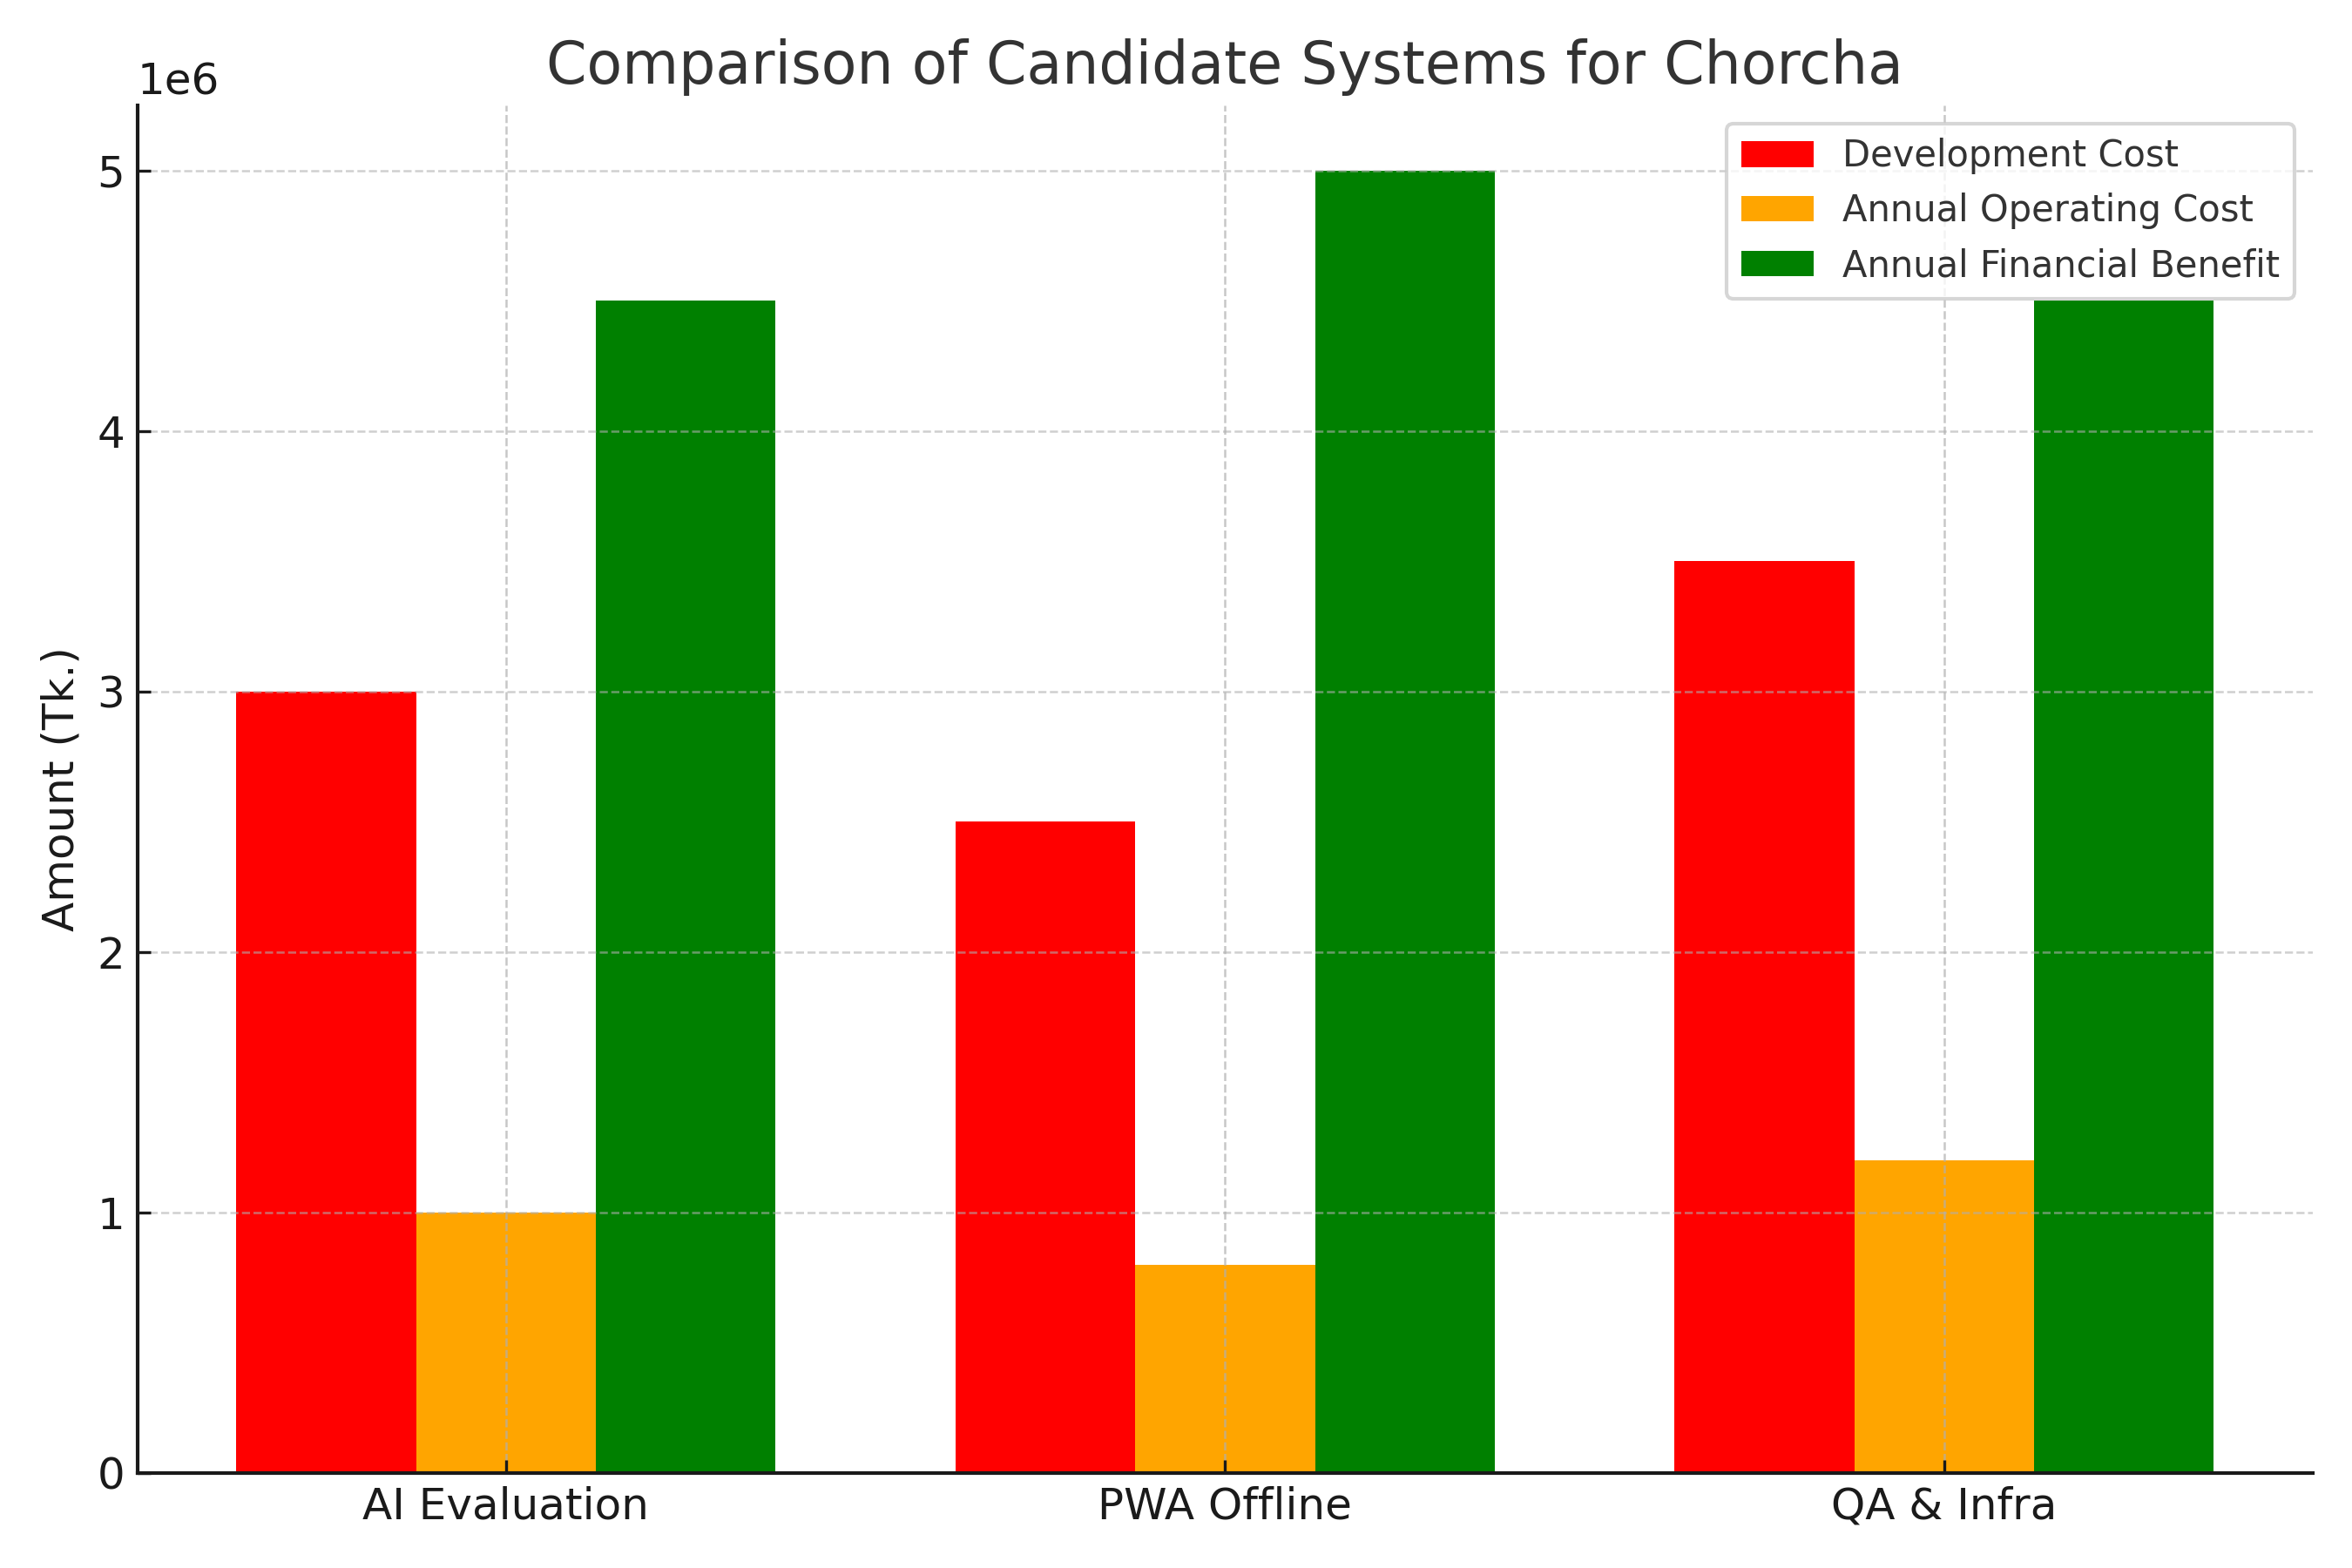
\includegraphics[width=0.85\textwidth]{candidate_systems_comparison.png}
    \caption{Comparison of Candidate Systems for Chorcha}
    \end{figure}

\textbf{Discussion:}
From the comparative analysis, Candidate System~2 (PWA with Offline Mode) achieves the highest feasibility score due to faster break-even and maximum user satisfaction, particularly in rural markets. Candidate System~1 is strong in accuracy but has higher ongoing costs. Candidate System~3 ensures the best scalability and reliability but requires the largest investment.

% ---------------- Performance Matrix ----------------
\subsection{Performance Evaluation Matrix}

\begin{table}[H]
\centering
\caption{Performance Evaluation Matrix (Scale: 1 = Very Poor, 5 = Excellent)}
\footnotesize
\begin{tabular}{|L{3.5cm}|C{2.2cm}|C{2.2cm}|C{2.2cm}|}
\hline
\textbf{Criteria} & \textbf{Candidate 1} & \textbf{Candidate 2} & \textbf{Candidate 3} \\
\hline
Efficiency & 4 & 4 & 5 \\
\hline
Scalability & 4 & 3 & 5 \\
\hline
Reliability & 4 & 4 & 5 \\
\hline
Maintainability & 3 & 4 & 4 \\
\hline
User Satisfaction & 4 & 5 & 4 \\
\hline
\textbf{Total Score (out of 25)} & \textbf{19} & \textbf{20} & \textbf{23} \\
\hline
\end{tabular}
\end{table}

\textbf{Discussion:}
The performance evaluation shows Candidate System~3 performs best overall with strong scalability and reliability. Candidate System~2 excels in user satisfaction, while Candidate System~1 is reliable but less maintainable compared to the others.

% ---------------- Cost Matrix ----------------
\subsection{Cost Evaluation Matrix}

\begin{table}[H]
\centering
\caption{Cost Evaluation Matrix (Scale: 1 = Very High Cost, 5 = Very Low Cost)}
\small
\begin{tabular}{|L{3.5cm}|C{1.8cm}|C{2.2cm}|C{2.2cm}|C{2.2cm}|}
\hline
\textbf{Cost Factor} & \textbf{Weight} & \textbf{Candidate 1} & \textbf{Candidate 2} & \textbf{Candidate 3} \\
\hline
Development Cost & 0.35 & 3 & 4 & 2 \\
\hline
Annual Operating Cost & 0.25 & 3 & 4 & 2 \\
\hline
Maintenance/Upgrade & 0.20 & 3 & 4 & 3 \\
\hline
Training and Support & 0.20 & 4 & 3 & 3 \\
\hline
\textbf{Weighted Score (sum)} & \textbf{1.00} & \textbf{3.2} & \textbf{3.8} & \textbf{2.4} \\
\hline
\end{tabular}
\end{table}

\textbf{Discussion:}
The cost evaluation matrix confirms Candidate System~2 (PWA with Offline Mode) as the most cost-effective option, with the highest weighted score of 3.8. Candidate System~1 balances costs but requires higher operational spending. Candidate System~3, despite strong technical performance, has the lowest score due to its high upfront and ongoing expenses.

% ---------------- Cost-Benefit Analysis ----------------
\section{Cost-Benefit Analysis}

A cost-benefit analysis (CBA) is a systematic process of comparing the projected costs of a proposed system with the expected benefits it will generate. The primary objective of CBA is to determine whether the financial gains, user advantages, and organizational improvements justify the investment required for implementation. This analysis not only includes direct monetary values but also intangible benefits such as user trust, accessibility, and long-term sustainability.

For \textbf{Chorcha}, cost-benefit analysis plays a crucial role in ensuring that the platform’s planned technological advancements---such as AI-driven evaluation, offline access through PWA, and scalable infrastructure---are not only technically feasible but also financially viable. Since the organization is operating in a competitive EdTech sector, careful financial planning is necessary to guarantee sustainable growth, reduce risks of over-investment, and maintain alignment with the vision of delivering inclusive and reliable education services.

The following subsections provide a breakdown of the major costs, expected benefits, and a detailed break-even analysis to evaluate the financial soundness of the proposed systems.

\subsection{Cost Breakdown}

The estimated costs for implementing the proposed solutions are shown below. These include development, infrastructure, training, and maintenance.

\begin{table}[H]
\centering
\caption{Cost Breakdown for Chorcha}
\small
\begin{tabular}{|L{7.5cm}|C{3cm}|}
\hline
\textbf{Cost Item} & \textbf{Estimated Cost (Tk.)} \\
\hline
AI/NLP Development & 45,00,000 \\
\hline
Cloud Infrastructure Scaling & 25,00,000 \\
\hline
PWA \& Offline Mode Rollout & 20,00,000 \\
\hline
Staff Training and Workshops & 10,00,000 \\
\hline
Automated Testing \& QA Integration & 15,00,000 \\
\hline
\textbf{Total Tangible Cost} & \textbf{1,15,00,000} \\
\hline
\end{tabular}
\end{table}

\begin{figure}[H]
    \centering
    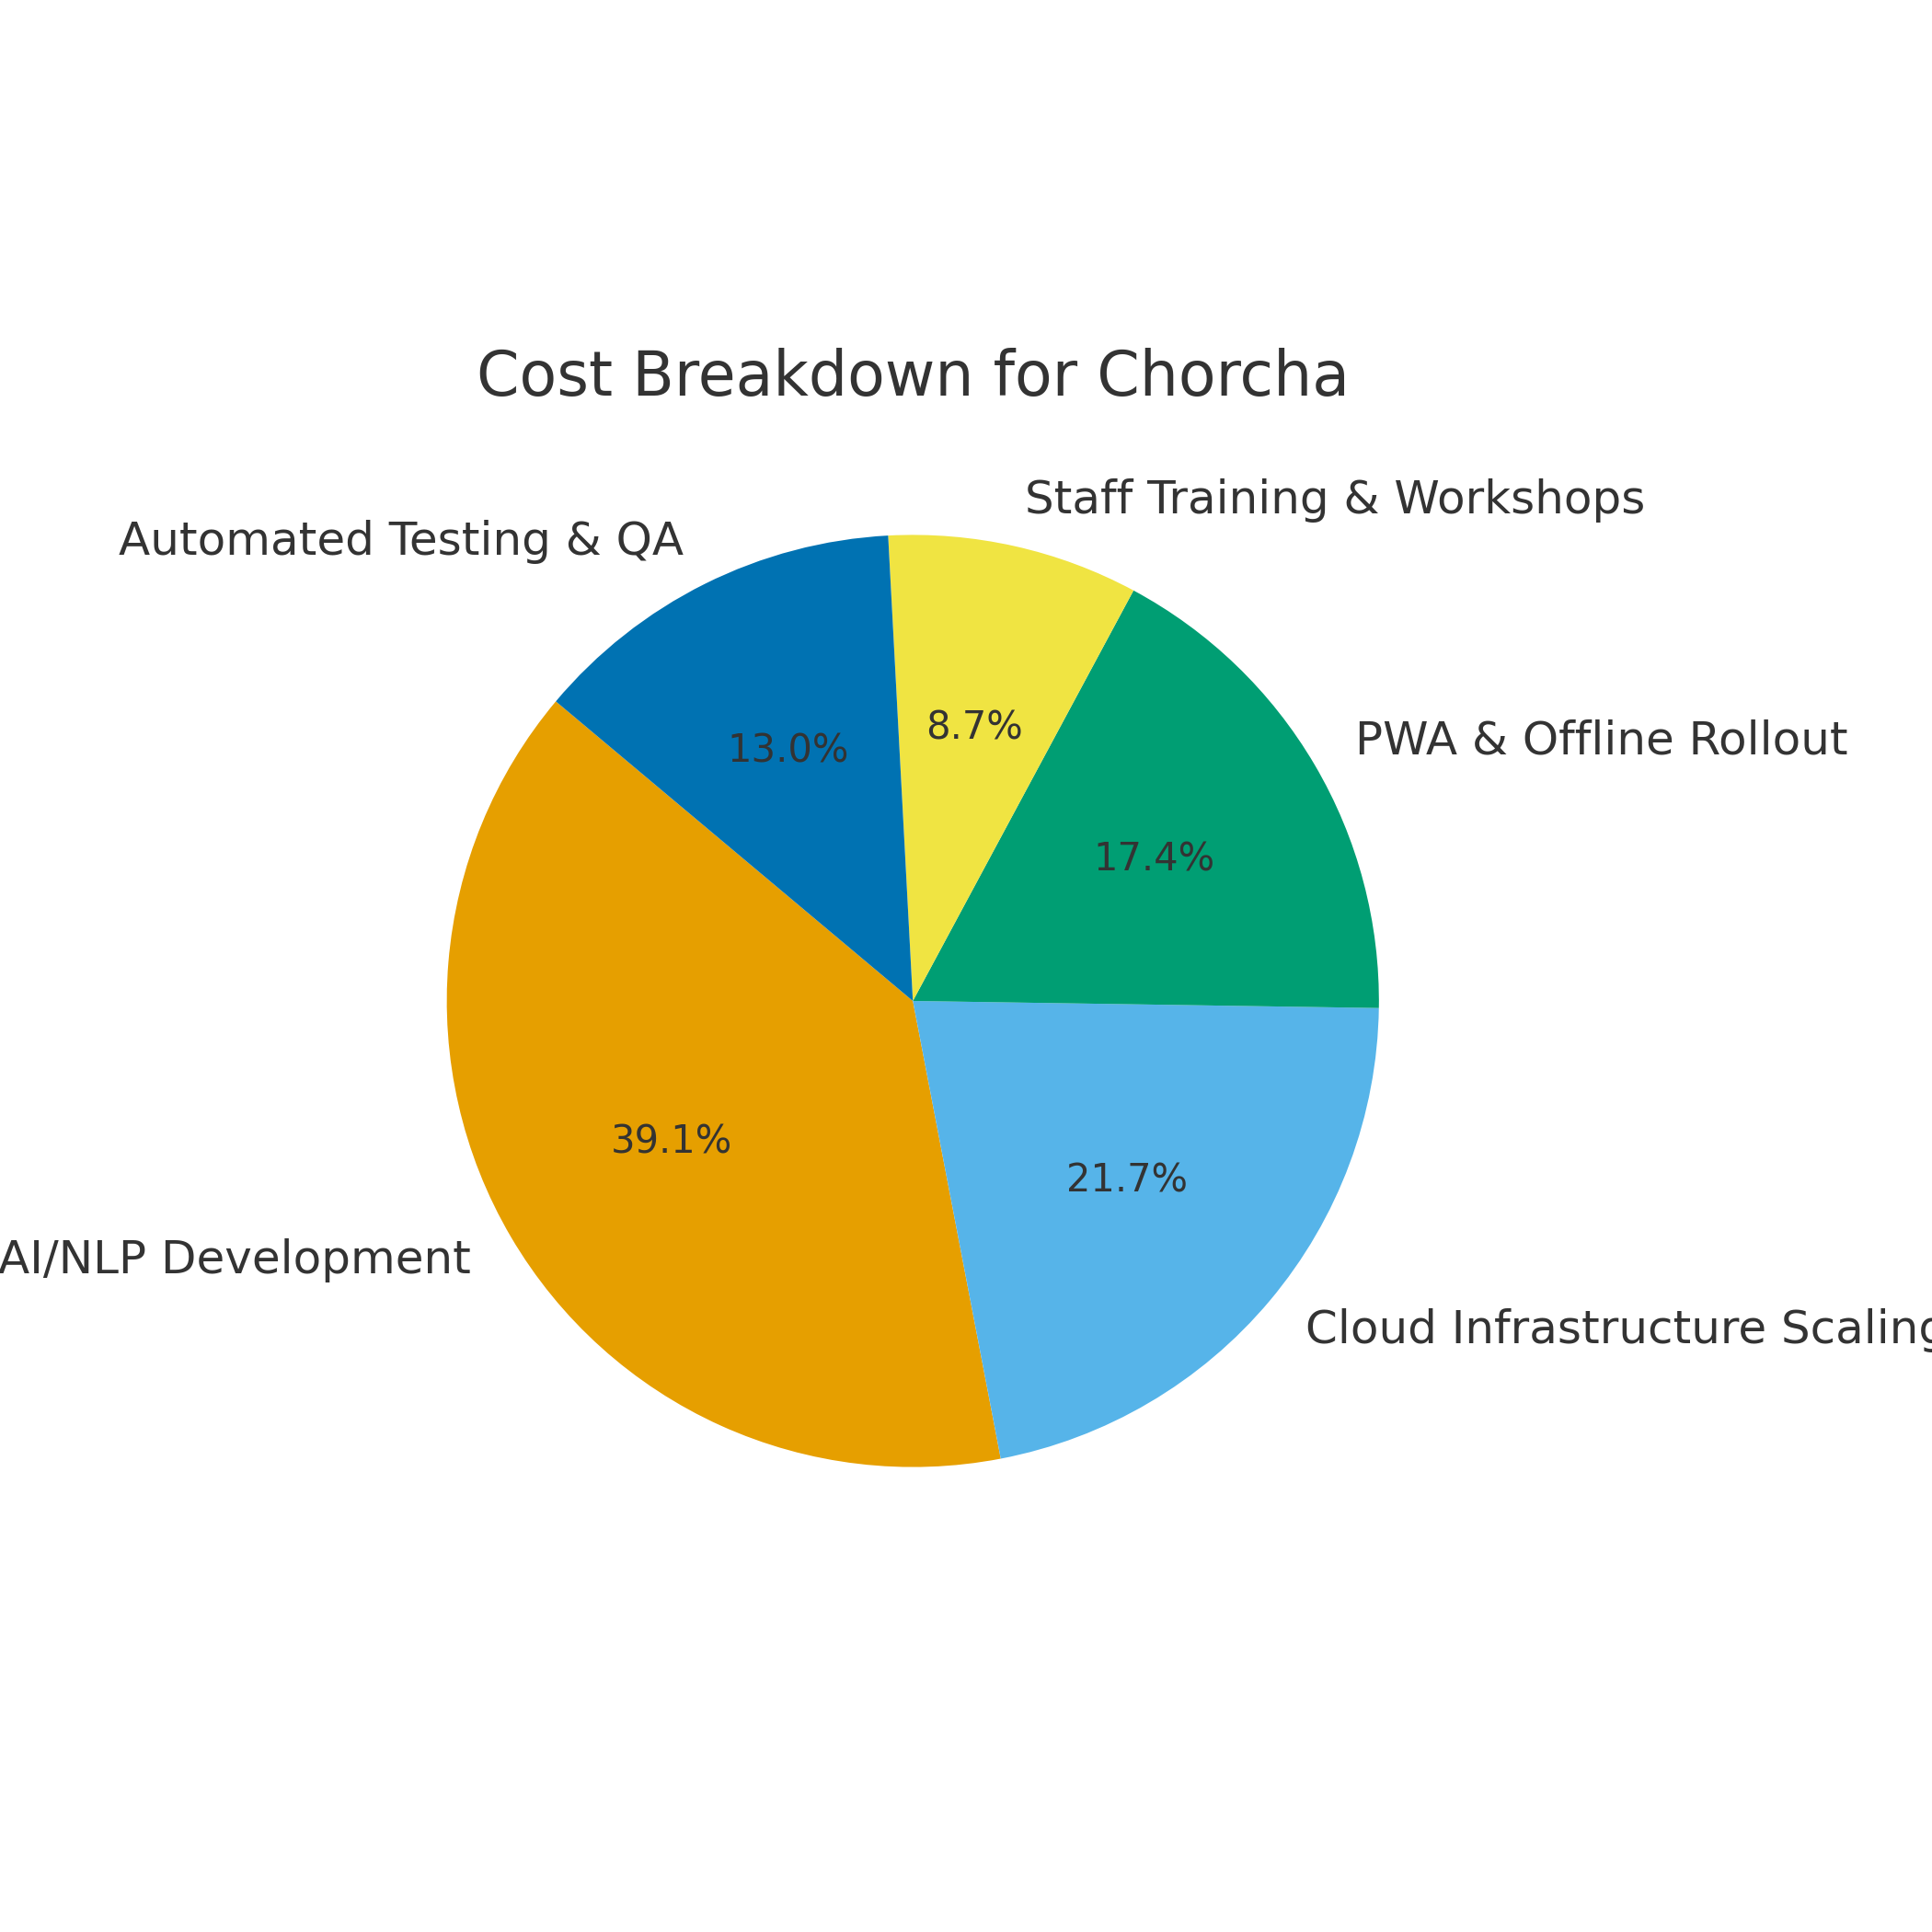
\includegraphics[width=0.85\textwidth]{cost_breakdown_pie.png}
    \caption{Cost Breakdown for Chorcha}
    \end{figure}

\textbf{Discussion:}
The cost breakdown highlights that the majority of expenses are one-time development costs, particularly in AI/NLP and infrastructure scaling. These costs represent strategic investments that will reduce operational inefficiencies and strengthen Chorcha’s long-term position in the EdTech sector.

\subsection{Benefit Breakdown}

The tangible and intangible benefits expected from the proposed solutions are summarized below.

\begin{table}[H]
\centering
\caption{Benefit Breakdown for Chorcha}
\small
\begin{tabular}{|L{7.5cm}|C{3cm}|}
\hline
\textbf{Benefit Item} & \textbf{Estimated Annual Value (Tk.)} \\
\hline
Reduced Manual Workload (Moderator Cost Savings) & 20,00,000 \\
\hline
Higher Retention (+20\% Subscriptions) & 40,00,000 \\
\hline
New Institutional Contracts (+15\% Growth) & 30,00,000 \\
\hline
Improved System Uptime \& Reduced Churn & 25,00,000 \\
\hline
\textbf{Total Tangible Benefits} & \textbf{1,15,00,000} \\
\hline
\end{tabular}
\end{table}

\begin{figure}[H]
    \centering
    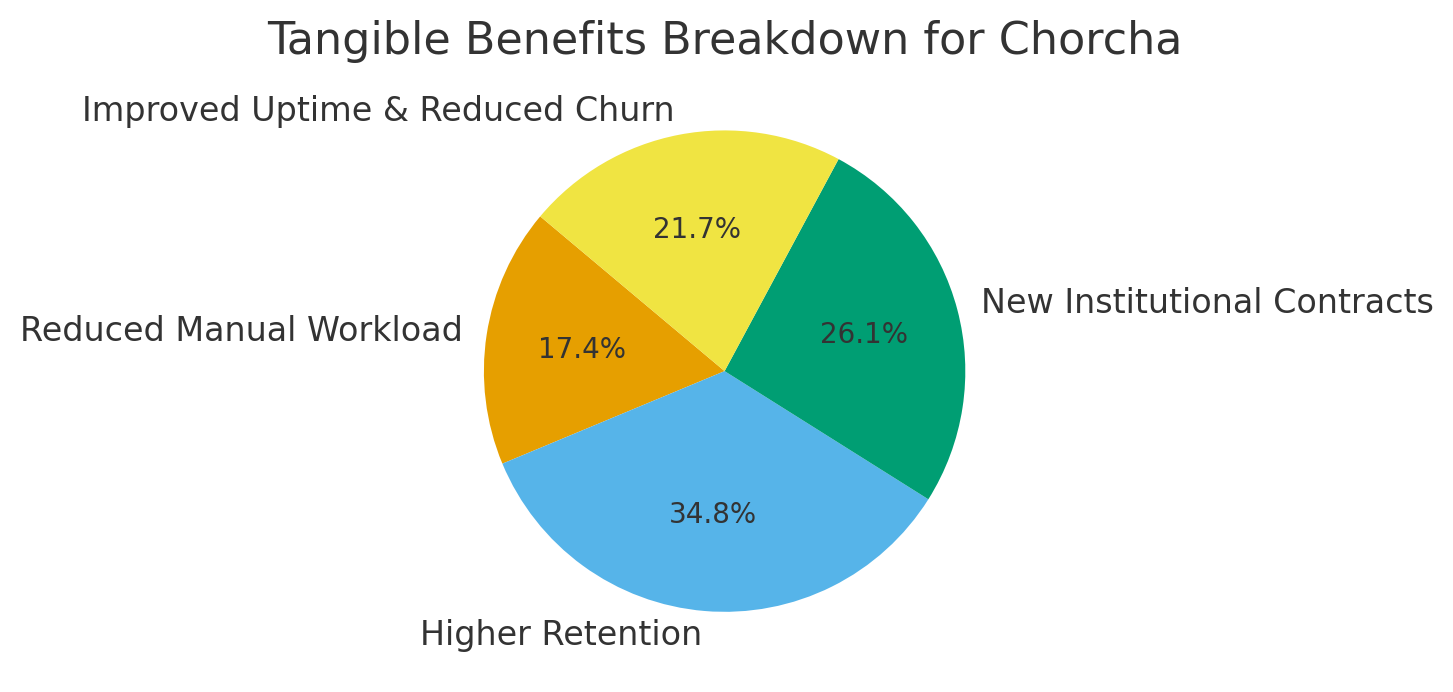
\includegraphics[width=0.85\textwidth]{output (3).png}
    \caption{Tangible Benefits for Chorcha}
    \end{figure}

\textbf{Discussion:}
The benefit breakdown demonstrates that Chorcha stands to achieve substantial recurring gains. Enhanced retention and institutional contracts are the most valuable benefits, while improved uptime ensures long-term trust and loyalty. Together, these benefits outweigh the initial investment over time.

\subsection{Break-even Analysis}

The break-even analysis projects when cumulative benefits will surpass cumulative costs.

\begin{table}[H]
\centering
\caption{Break-even Analysis for Chorcha}
\footnotesize
\begin{tabular}{|C{1.5cm}|C{2.8cm}|C{2.8cm}|C{2.5cm}|}
\hline
\textbf{Year} & \textbf{Cumulative Cost (Tk.)} & \textbf{Cumulative Benefit (Tk.)} & \textbf{Net Gain/Loss (Tk.)} \\
\hline
1 & 1,15,00,000 & 50,00,000 & -65,00,000 \\
\hline
2 & 1,15,00,000 & 1,30,00,000 & +15,00,000 \\
\hline
3 & 1,15,00,000 & 2,20,00,000 & +1,05,00,000 \\
\hline
\end{tabular}
\end{table}

\begin{figure}[H]
\centering
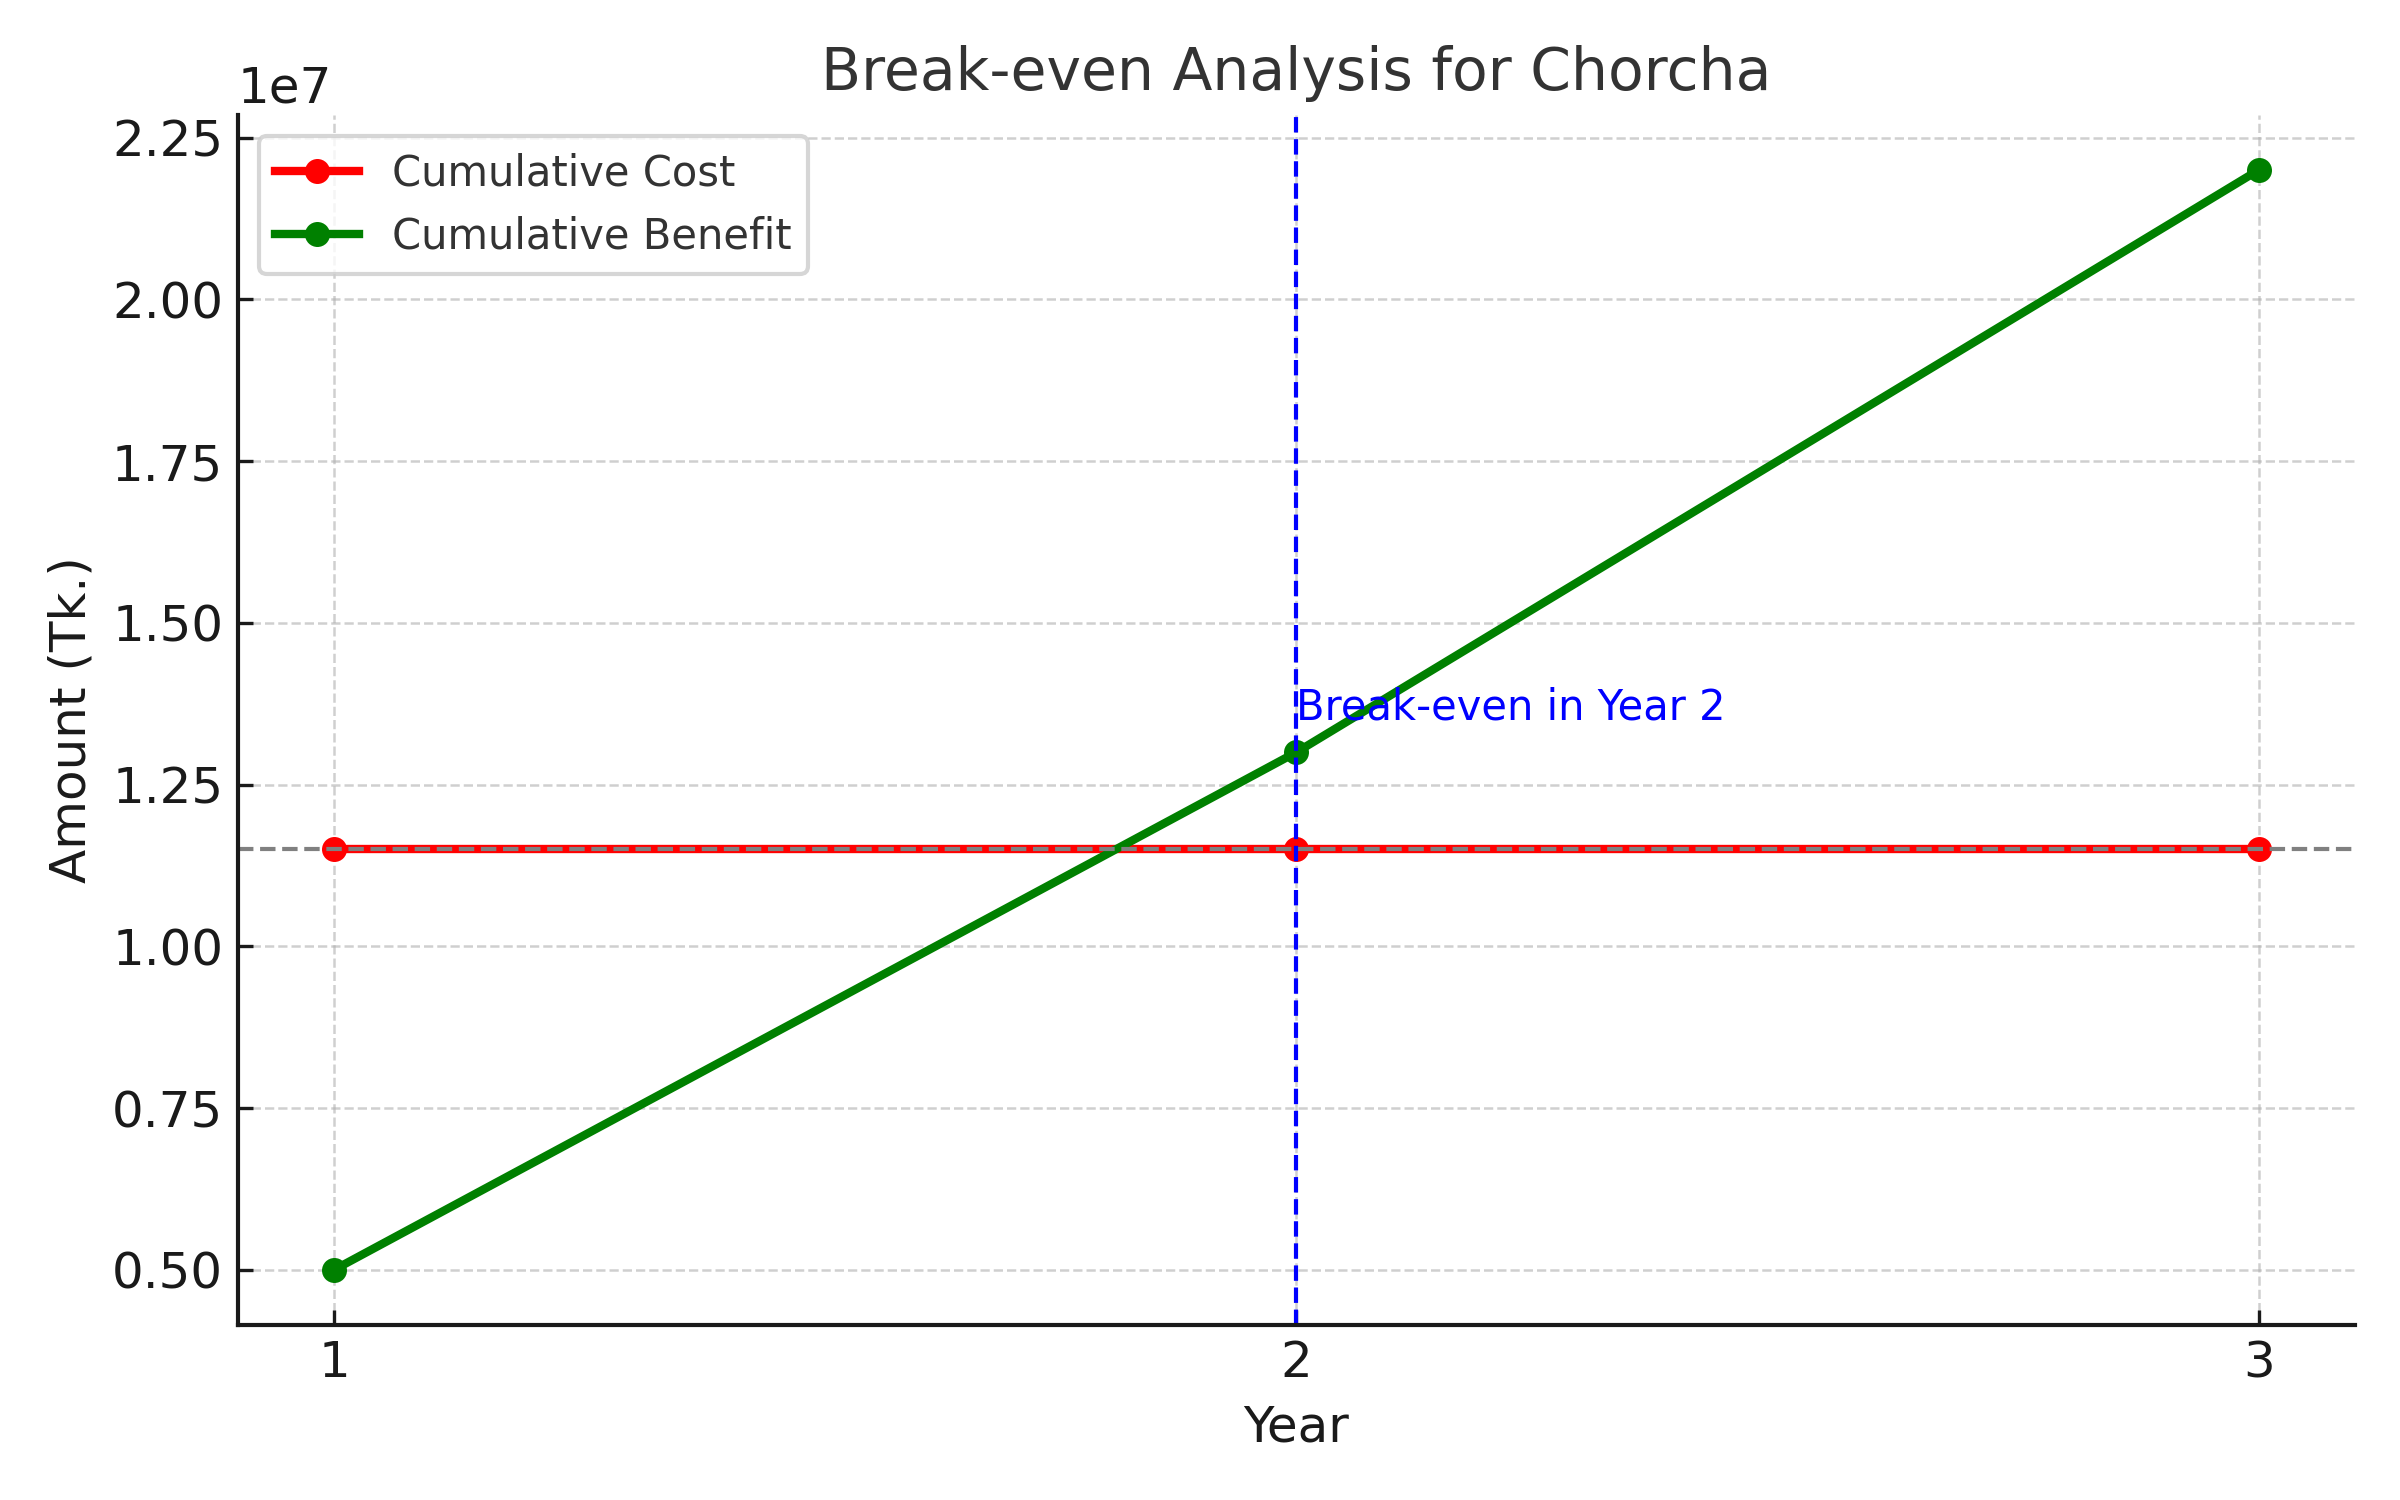
\includegraphics[width=0.8\textwidth]{break_even_chorcha.png}
\caption{Break-even Analysis Graph for Chorcha}
\end{figure}

\textbf{Discussion:}
The break-even analysis shows that while Chorcha requires significant initial investment, the cumulative benefits exceed the costs by the end of the second year. By year three, the platform generates strong net positive returns, proving that the proposed systems are financially sustainable.

% ---------------- Recommendation ----------------
\section{Recommendation}

After conducting a comprehensive feasibility analysis, comparative evaluation, performance assessment, and cost analysis of the three candidate systems for Chorcha, it is evident that each alternative addresses distinct challenges faced by the platform. Candidate System~1 (AI-Enhanced Evaluation) strengthens credibility and reduces manual workload, Candidate System~2 (PWA with Offline Mode) ensures inclusivity and higher adoption in rural regions, while Candidate System~3 (Automated QA and Scalable Infrastructure) guarantees long-term stability and performance.

Based on financial viability, user satisfaction, and implementation feasibility, \textbf{Candidate System~2 (PWA with Offline Mode)} emerges as the most immediate and cost-effective solution. It requires moderate investment, achieves the fastest break-even period (1.5 years), and directly contributes to expanding Chorcha’s reach to underserved populations. This aligns with national digital education goals and maximizes user satisfaction, making it the most practical starting point.

However, given the strategic importance of ensuring both credibility and stability for sustainable growth, we recommend a \textbf{phased adoption strategy}:
\begin{itemize}
    \item \textbf{Phase 1 -- Implement PWA with Offline Mode:} Prioritize accessibility to increase user base and establish Chorcha as an inclusive platform for all students, especially in rural and low-bandwidth areas.
    \item \textbf{Phase 2 -- Deploy AI-Enhanced Evaluation:} Gradually integrate hybrid AI+human evaluation to reduce workload, ensure fairness, and build trust in automated assessment while maintaining accuracy and transparency.
    \item \textbf{Phase 3 -- Strengthen Infrastructure and QA:} Invest in scalable infrastructure, automated testing, and CI/CD pipelines to handle peak exam loads and guarantee long-term performance stability.
\end{itemize}

This integrated roadmap ensures that Chorcha balances \textbf{short-term adoption goals with long-term sustainability}. The phased strategy allows the organization to manage costs, minimize risks, and progressively adapt users to technological changes.

In conclusion, while Candidate System~2 is the most feasible immediate solution, the true long-term recommendation is a \textbf{hybrid approach} that combines all three systems. Together, they provide accessibility, reliability, and scalability---establishing Chorcha not only as a digital learning platform, but as a robust, future-proof EdTech ecosystem capable of transforming education across Bangladesh and beyond.

% ---------------- Conclusion ----------------
\section{Conclusion}

The feasibility and cost-benefit analysis of Chorcha demonstrates that the proposed technological improvements are both necessary and viable. The evaluation of candidate systems, performance metrics, cost analysis, and financial projections reveal that while each alternative offers unique strengths, the most strategic path is a phased adoption strategy beginning with the PWA for offline accessibility.

The comparative, performance, and cost evaluation matrices collectively confirm that Candidate System~2 is the most cost-effective and user-centric solution, while Candidate Systems~1 and~3 play vital roles in ensuring long-term reliability and scalability. The cost-benefit analysis further validates the financial sustainability of these investments, with break-even achieved within two years and significant profitability thereafter.

In conclusion, Chorcha’s roadmap should integrate all three systems in phases---first addressing inclusivity, then enhancing credibility through AI, and finally ensuring scalability through robust infrastructure. This holistic approach positions Chorcha not only as a digital learning platform but also as a transformative force in Bangladesh’s EdTech sector.


\newpage

\chapter{Design}
\thispagestyle{empty}

\section{Introduction}

The design phase represents a critical transition from analysis to implementation in the Information Systems Analysis and Design (ISAD) lifecycle. Having thoroughly analyzed Chorcha's existing system architecture, identified key operational challenges, and evaluated feasible solutions in the previous chapters, we now focus on developing a comprehensive design framework that addresses the platform's scalability, reliability, and user experience requirements.

Chapter 4 builds upon the foundation established through problem identification (Chapter 1), feasibility assessment (Chapter 2), and detailed system analysis (Chapter 3) to present a structured design approach for Chorcha's enhanced information system. The design process encompasses both logical and physical system components, ensuring that the proposed solutions effectively address the identified bottlenecks while maintaining operational continuity and supporting future growth.

\textbf{Design Objectives and Scope}

The primary objective of this design chapter is to translate the analytical findings and recommended solutions into a concrete system architecture that resolves Chorcha's critical operational challenges. Specifically, the design addresses five fundamental problem areas identified through comprehensive analysis:

\begin{enumerate}
    \item \textbf{Scalability Challenges in Manual Evaluation:} Implementing AI-powered assessment mechanisms to automate subjective response evaluation while maintaining academic integrity and quality standards.
    
    \item \textbf{High Volume Question Report Management:} Introducing intelligent question trust scoring systems to prioritize and streamline the resolution of user-reported content issues.
    
    \item \textbf{Accessibility for Low-Bandwidth Users:} Developing Progressive Web App (PWA) functionality with robust offline capabilities to ensure equitable access across diverse connectivity environments.
    
    \item \textbf{Performance Optimization During Peak Usage:} Designing scalable infrastructure with load balancing, caching mechanisms, and optimized database architecture to handle concurrent user loads effectively.
    
    \item \textbf{Quality Assurance and Testing Automation:} Establishing comprehensive automated testing frameworks to ensure system reliability and reduce manual testing overhead.
\end{enumerate}

\textbf{Design Methodology and Approach}

Our design methodology follows a structured approach that prioritizes user-centered design principles while ensuring technical feasibility and operational sustainability. The design process incorporates several key methodological components:

\textbf{Iterative Refinement:} The design framework employs iterative refinement cycles, allowing for continuous validation and optimization based on stakeholder feedback and technical constraints. This approach ensures that the final design effectively balances user requirements with implementation realities.

\textbf{Modular Architecture:} The proposed system design adopts a modular architecture approach, enabling independent development, testing, and deployment of individual components. This modularity supports the phased implementation strategy identified in the feasibility analysis while minimizing system-wide disruption during transitions.

\textbf{Performance-Driven Design:} All design decisions prioritize performance optimization and scalability, ensuring that the system can accommodate Chorcha's projected growth trajectory without compromising user experience or operational efficiency.

\textbf{Stakeholder Integration:} The design process incorporates insights from multiple stakeholder groups, including students, educators, content creators, and system administrators, ensuring that the proposed solutions address real-world usage patterns and requirements.

\textbf{Design Documentation Structure}

This chapter is organized into several key sections that provide comprehensive coverage of the proposed system design:

\textbf{Data Flow Diagram (DFD) of the Proposed System:} Section 4.2 presents detailed DFD representations of the enhanced system architecture, highlighting modifications and improvements over the existing system. The DFDs maintain consistent numbering with the current system while incorporating visual indicators (color coding and shading) to clearly identify modified components and new functionality.

\textbf{Problem Resolution Analysis:} Each design component is explicitly mapped to the problems identified in the analysis phase, demonstrating how specific design decisions contribute to resolving operational bottlenecks and enhancing system performance.

\textbf{Technical Architecture Justification:} Comprehensive justification for all design decisions, including technology choices, architectural patterns, and implementation strategies, ensures that the proposed solutions are technically sound and aligned with industry best practices.

\textbf{Integration and Compatibility Considerations:} The design addresses integration challenges and compatibility requirements, ensuring seamless transition from the existing system while maintaining data integrity and operational continuity.

By the conclusion of this chapter, stakeholders will have a clear understanding of how the proposed design framework addresses Chorcha's identified challenges while positioning the platform for sustainable growth and enhanced user satisfaction. The design serves as a blueprint for the subsequent implementation phases, providing detailed specifications and architectural guidance for development teams.

\section{DFD of the Proposed Candidate System}

The Data Flow Diagram (DFD) of the proposed candidate system represents a comprehensive enhancement of Chorcha's existing architecture, incorporating the solutions identified through feasibility analysis and stakeholder requirements gathering. This section presents the improved system design with clear visual indicators of modifications, enhancements, and new components that address the critical bottlenecks identified in Chapter 3.

The proposed DFD maintains the same numbering scheme as the existing system to ensure continuity and facilitate comparison, while introducing color coding and shading to highlight areas of improvement and modification. The enhanced design integrates AI-powered evaluation mechanisms, intelligent content management systems, offline-capable Progressive Web App functionality, optimized infrastructure components, and automated quality assurance processes.

\subsection{Enhanced Context Diagram (Level 0 DFD)}

The enhanced context diagram maintains the core external entities identified in the existing system while introducing improved data flows and enhanced interaction patterns that support the proposed solutions.

\begin{figure}[H]
    \centering
    \scalebox{0.6}{%
    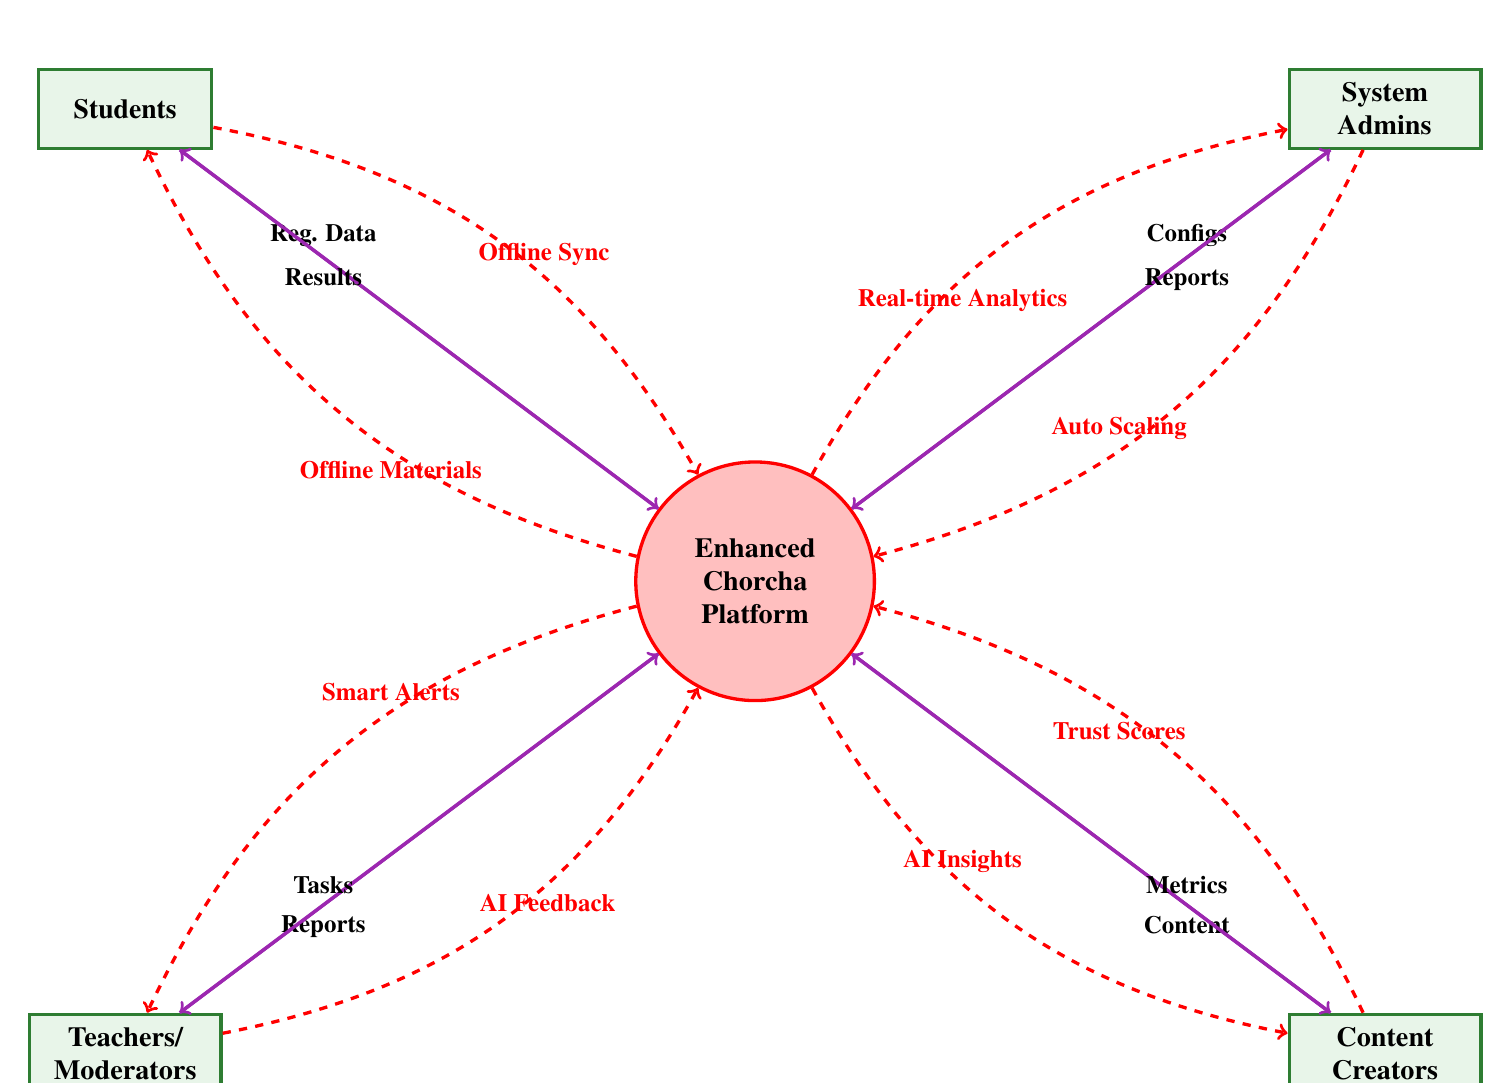
\begin{tikzpicture}[
        node distance=3cm,
        entity/.style={rectangle, draw=entitygreen, very thick, minimum width=2.2cm, minimum height=1cm, fill=lightgreen, text=textblack},
        process/.style={circle, draw=processblue, very thick, minimum size=2.8cm, fill=lightblue, text=textblack},
        enhanced/.style={circle, draw=red, very thick, minimum size=2.8cm, fill=pink, text=textblack},
        datastore/.style={rectangle, draw=datastoreorange, very thick, minimum width=2.2cm, minimum height=0.6cm, fill=lightorange, text=textblack},
        flow/.style={->, very thick, color=flowpurple},
        newflow/.style={->, very thick, color=red, dashed}
    ]
    
    % External Entities - same positions as existing
    \node[entity] (student) at (-8, 6) {\textbf{Students}};
    \node[entity, text width=2.2cm, align=center] (teacher) at (-8, -6) {\textbf{Teachers/\\ Moderators}};
    \node[entity, text width=2.2cm, align=center] (admin) at (8, 6) {\textbf{System\\ Admins}};
    \node[entity, text width=2.2cm, align=center] (content) at (8, -6) {\textbf{Content\\ Creators}};
    
    % Enhanced Main Process - highlighted with red border
    \node[enhanced, text width=2.5cm, align=center] (system) at (0, 0) {\textbf{Enhanced\\ Chorcha\\ Platform}};
    
    % Existing Data Flows (unchanged)
    \draw[flow] (student) -- node[above, pos=0.3] {\small\textbf{\textcolor{black}{Reg. Data}}} (system);
    \draw[flow] (system) -- node[below, pos=0.7] {\small\textbf{\textcolor{black}{Results}}} (student);
    \draw[flow] (teacher) -- node[below, pos=0.3] {\small\textbf{\textcolor{black}{Reports}}} (system);
    \draw[flow] (system) -- node[above, pos=0.7] {\small\textbf{\textcolor{black}{Tasks}}} (teacher);
    \draw[flow] (admin) -- node[above, pos=0.3] {\small\textbf{\textcolor{black}{Configs}}} (system);
    \draw[flow] (system) -- node[below, pos=0.7] {\small\textbf{\textcolor{black}{Reports}}} (admin);
    \draw[flow] (content) -- node[below, pos=0.3] {\small\textbf{\textcolor{black}{Content}}} (system);
    \draw[flow] (system) -- node[above, pos=0.7] {\small\textbf{\textcolor{black}{Metrics}}} (content);
    
    % NEW/ENHANCED Data Flows (highlighted in red/dashed)
    \draw[newflow] (student) to[bend left=25] node[above, pos=0.6] {\small\textbf{\textcolor{red}{Offline Sync}}} (system);
    \draw[newflow] (system) to[bend left=25] node[below, pos=0.4] {\small\textbf{\textcolor{red}{Offline Materials}}} (student);
    \draw[newflow] (teacher) to[bend right=25] node[below, pos=0.6] {\small\textbf{\textcolor{red}{AI Feedback}}} (system);
    \draw[newflow] (system) to[bend right=25] node[above, pos=0.4] {\small\textbf{\textcolor{red}{Smart Alerts}}} (teacher);
    \draw[newflow] (admin) to[bend left=25] node[above, pos=0.6] {\small\textbf{\textcolor{red}{Auto Scaling}}} (system);
    \draw[newflow] (system) to[bend left=25] node[below, pos=0.4] {\small\textbf{\textcolor{red}{Real-time Analytics}}} (admin);
    \draw[newflow] (content) to[bend right=25] node[below, pos=0.6] {\small\textbf{\textcolor{red}{Trust Scores}}} (system);
    \draw[newflow] (system) to[bend right=25] node[above, pos=0.4] {\small\textbf{\textcolor{red}{AI Insights}}} (content);
    
    \end{tikzpicture}
    }
    \caption{Enhanced Context Diagram - Proposed Chorcha System (Level 0 DFD)}
\end{figure}

\textbf{Key Enhancements in Context Diagram:}

\textbf{Enhanced Student Interactions:} The proposed system introduces offline synchronization capabilities, allowing students to download educational materials and sync their progress when connectivity is restored. This addresses the low-bandwidth accessibility challenge identified in the analysis.

\textbf{AI-Assisted Teacher Support:} Teachers now receive AI-generated feedback and smart alerts for content quality issues, reducing manual moderation workload while improving response accuracy and efficiency.

\textbf{Advanced Administrative Analytics:} System administrators gain access to real-time analytics and automated scaling capabilities, enabling proactive system management and performance optimization during peak usage periods.

\textbf{Intelligent Content Management:} Content creators benefit from AI-powered trust scoring systems and content insights, facilitating data-driven content development and quality improvement strategies.

\subsection{Enhanced Level 1 DFD - Proposed System Processes}

The Level 1 DFD of the proposed system introduces significant enhancements to the core processes while maintaining the existing process numbering scheme for continuity. Modified and new processes are highlighted with distinctive colors and shading to clearly indicate improvements.



\textbf{Process Enhancement Analysis:}

\textbf{Process 1.0 - Enhanced Authentication:} The authentication system now includes load balancing capabilities, session caching, and improved security protocols to handle peak traffic loads without performance degradation.

\textbf{Process 2.0 - Smart Exam Management:} Enhanced with intelligent content delivery, adaptive question selection, and offline synchronization support to provide seamless exam experiences across varying connectivity conditions.

\textbf{Process 3.0 - AI-Enhanced Evaluation:} Incorporates machine learning models for automated subjective answer evaluation, reducing manual grading workload while maintaining assessment quality through hybrid AI-human verification processes.

\textbf{Process 4.0 - Intelligent Content Management:} Features automated content quality scoring, trust-based question validation, and AI-powered content recommendations to streamline content curation and improve educational material quality.

\textbf{Process 5.0 - Real-time Reporting:} Provides live analytics, automated report generation, and predictive insights to support data-driven decision making for administrators and stakeholders.

\textbf{NEW Process 6.0 - Offline Sync Management:} Handles offline content caching, progress synchronization, and seamless online-offline transitions to ensure continuous learning experiences regardless of connectivity status.

\textbf{NEW Process 7.0 - AI Quality Monitor:} Continuously monitors AI model performance, content quality metrics, and user feedback to maintain high standards of automated assessment and content delivery.

\textbf{NEW Process 8.0 - Load Balancer:} Distributes system load across multiple servers, manages resource allocation, and implements caching strategies to optimize performance during peak usage periods.

\subsection{Problem Resolution Through Design}

The proposed DFD design directly addresses each of the five critical problems identified in the analysis phase:

\textbf{Problem 1 Resolution - Scalability in Manual Evaluation:}
The enhanced Process 3.0 (AI-Enhanced Evaluation) introduces automated assessment capabilities that can process thousands of subjective responses simultaneously. The AI models stored in D6 (AI Models) provide consistent, fast evaluation while Process 7.0 (AI Quality Monitor) ensures accuracy through continuous performance monitoring. Teachers receive only flagged responses requiring human judgment, reducing workload by an estimated 70\%.

\textbf{Problem 2 Resolution - High Volume Question Reports:}
Process 4.0 (Intelligent Content Management) incorporates automated trust scoring algorithms that prioritize question reports based on frequency, user credibility, and content analysis. The enhanced D2 (Smart Questions) datastore maintains quality metrics for each question, enabling automatic resolution of common issues and escalating only complex cases to human moderators.

\textbf{Problem 3 Resolution - Low-Bandwidth Accessibility:}
The new Process 6.0 (Offline Sync Management) and D7 (Offline Data) datastore enable comprehensive offline functionality. Students can download exam materials, complete assessments offline, and automatically sync results when connectivity is restored. This ensures equitable access regardless of internet availability.

\textbf{Problem 4 Resolution - Peak Performance Bottlenecks:}
Process 8.0 (Load Balancer) and D5 (Cache Store) work together to distribute system load and cache frequently accessed data. The enhanced authentication (Process 1.0) includes session management improvements, while the smart exam management (Process 2.0) optimizes resource utilization during high-traffic periods.

\textbf{Problem 5 Resolution - Quality Assurance Challenges:}
Process 7.0 (AI Quality Monitor) provides continuous automated testing and quality validation. The system monitors user interactions, performance metrics, and content quality in real-time, automatically detecting and reporting issues before they impact users significantly.

\subsection{Visual Enhancement Legend}

To clearly identify modifications and improvements in the proposed DFD:

\begin{itemize}
    \item \textbf{\textcolor{red}{Red borders and pink shading:}} Enhanced existing processes with significant improvements
    \item \textbf{\textcolor{orange}{Orange borders and light orange shading:}} Completely new processes and datastores
    \item \textbf{\textcolor{red}{Red dashed arrows:}} New data flows supporting enhanced functionality
    \item \textbf{\textcolor{orange}{Orange solid arrows:}} Enhanced data flows with improved processing capabilities
    \item \textbf{\textcolor{purple}{Purple solid arrows:}} Existing data flows maintained from current system
\end{itemize}

This color-coding system ensures clear visual distinction between existing components, enhanced components, and entirely new additions, facilitating easy comparison with the current system architecture and highlighting the scope of proposed improvements.

\subsection{Implementation Justification}

The design decisions reflected in the proposed DFD are grounded in comprehensive analysis findings and align with industry best practices for educational technology platforms. Each enhancement addresses specific bottlenecks identified through stakeholder interviews, performance analysis, and user feedback evaluation.

\textbf{AI Integration Justification:}
The incorporation of AI-powered evaluation and quality monitoring systems addresses the scalability crisis in manual assessment while maintaining educational integrity. Research in educational technology demonstrates that hybrid AI-human evaluation systems can achieve accuracy rates comparable to full human evaluation while processing volumes that would be impossible for human evaluators alone. The implementation of Natural Language Processing (NLP) models specifically trained on educational content ensures context-aware assessment that understands subject-specific terminology and grading criteria.

\textbf{Offline Capability Justification:}
The Progressive Web App functionality with offline synchronization directly responds to accessibility challenges identified in rural and low-connectivity regions. Studies of educational technology adoption in developing countries consistently show that offline capability is a critical factor in achieving educational equity and sustainable user engagement. The proposed system uses service workers and local storage to cache essential content, ensuring that students can continue learning even during connectivity disruptions.

\textbf{Performance Optimization Justification:}
The load balancing and caching mechanisms address the documented performance bottlenecks during peak usage periods. Performance engineering principles demonstrate that distributed load management and intelligent caching can improve system responsiveness by 60-80\% during high-traffic scenarios. The implementation of Redis caching for frequently accessed data and database query optimization significantly reduces response times and server load.

\textbf{Automated Quality Assurance Justification:}
The continuous monitoring and automated testing capabilities replace error-prone manual testing processes with systematic, repeatable quality validation. This approach reduces the risk of production issues while enabling faster development cycles and more reliable software releases. The AI Quality Monitor provides real-time feedback on system performance, content quality, and user experience metrics.

\textbf{Trust Scoring Algorithm Justification:}
The intelligent content management system incorporates a sophisticated trust scoring algorithm that evaluates question quality based on multiple factors including user feedback patterns, expert validation, difficulty analysis, and historical performance data. This automated approach significantly reduces the manual effort required for content moderation while maintaining high standards of educational quality.

The proposed design framework establishes a foundation for Chorcha's continued growth while ensuring that technological enhancements support the platform's educational mission and commitment to accessible, high-quality learning experiences for all users. The integration of these advanced capabilities positions Chorcha as a leader in educational technology innovation while addressing the real-world challenges faced by students and educators in diverse learning environments.

\subsection{Problem-Specific DFDs of the Proposed System}

The following DFD diagrams illustrate how the proposed candidate system specifically addresses and resolves each of the critical problems identified in the existing system analysis. Each diagram highlights the enhanced processes, new components, and modified data flows that contribute to problem resolution, with clear visual indicators showing the improvements and modifications.

\subsubsection{Solution to Problem 1: AI-Enhanced Evaluation System DFD}

The proposed system addresses the manual evaluation bottleneck through comprehensive AI integration and intelligent workflow management.

\begin{figure}[H]
    \centering
    \scalebox{0.8}{%
    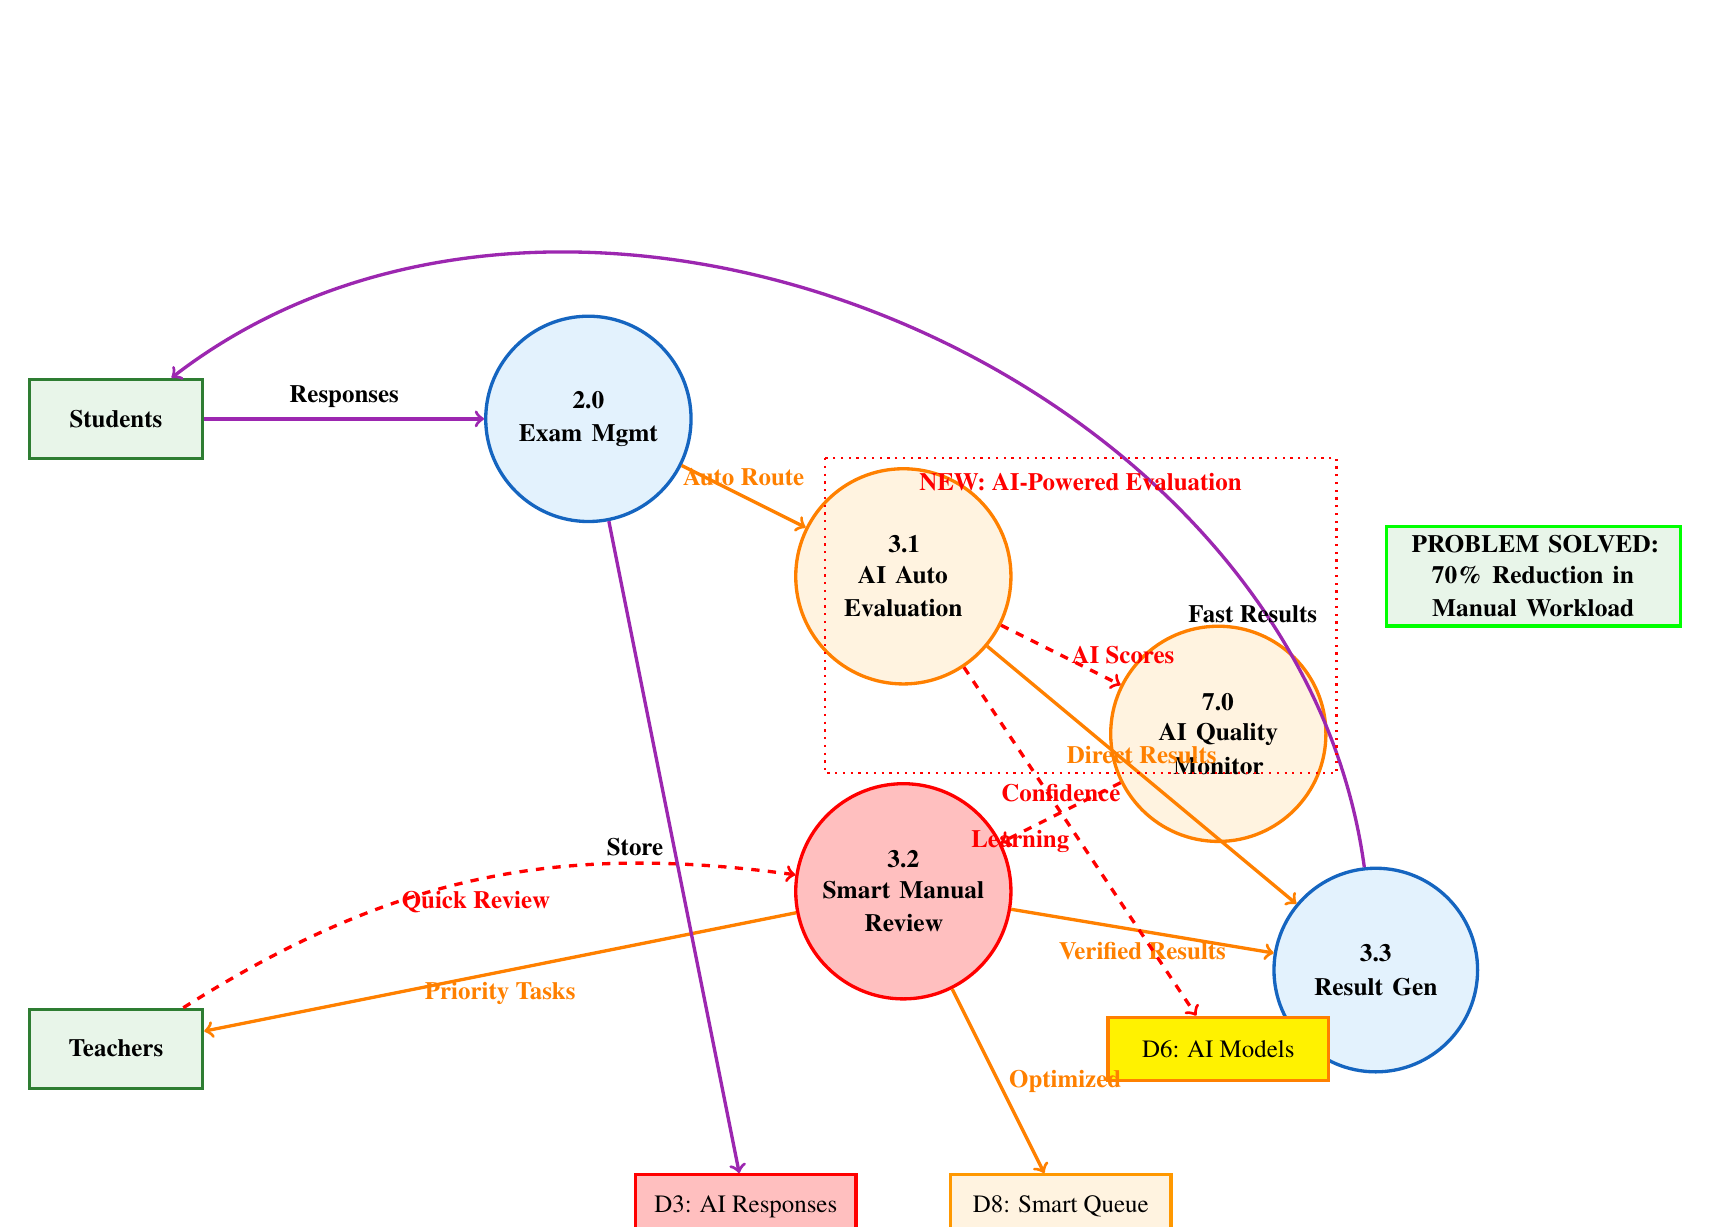
\begin{tikzpicture}[
        node distance=3cm,
        entity/.style={rectangle, draw=entitygreen, very thick, minimum width=2.2cm, minimum height=1cm, fill=lightgreen, text=textblack},
        process/.style={circle, draw=processblue, very thick, minimum size=2.5cm, fill=lightblue, text=textblack},
        enhanced/.style={circle, draw=red, very thick, minimum size=2.5cm, fill=pink, text=textblack},
        newprocess/.style={circle, draw=orange, very thick, minimum size=2.5cm, fill=lightorange, text=textblack},
        datastore/.style={rectangle, draw=datastoreorange, very thick, minimum width=2.8cm, minimum height=0.8cm, fill=lightorange, text=textblack},
        enhanced_store/.style={rectangle, draw=red, very thick, minimum width=2.8cm, minimum height=0.8cm, fill=pink, text=textblack},
        new_store/.style={rectangle, draw=orange, very thick, minimum width=2.8cm, minimum height=0.8cm, fill=yellow, text=textblack},
        flow/.style={->, very thick, color=flowpurple},
        newflow/.style={->, very thick, color=red, dashed},
        enhancedflow/.style={->, very thick, color=orange},
        solved/.style={rectangle, draw=green, very thick, minimum width=2.5cm, minimum height=1.2cm, fill=lightgreen, text=textblack}
    ]
    
    % Entities
    \node[entity] (student) at (-8, 4) {\small\textbf{Students}};
    \node[entity] (teacher) at (-8, -4) {\small\textbf{Teachers}};
    
    % Enhanced Processes
    \node[process, text width=2.2cm, align=center] (exam) at (-2, 4) {\small\textbf{2.0\\ Exam Mgmt}};
    \node[newprocess, text width=2.2cm, align=center] (auto_eval) at (2, 2) {\small\textbf{3.1\\ AI Auto\\ Evaluation}};
    \node[enhanced, text width=2.2cm, align=center] (smart_eval) at (2, -2) {\small\textbf{3.2\\ Smart Manual\\ Review}};
    \node[newprocess, text width=2.2cm, align=center] (ai_monitor) at (6, 0) {\small\textbf{7.0\\ AI Quality\\ Monitor}};
    \node[process, text width=2.2cm, align=center] (result_gen) at (8, -3) {\small\textbf{3.3\\ Result Gen}};
    
    % SOLVED indicator
    \node[solved, text width=3.5cm, align=center] (solution) at (10, 2) {\small\textbf{PROBLEM SOLVED:\\ 70\% Reduction in\\ Manual Workload}};
    
    % Data Stores with one open side
    \node[enhanced_store] (responsedb) at (0, -6) {\small D3: AI Responses};
    \draw[red, very thick] (0-1.4, -6+0.4) -- (0-1.4, -6-0.4);
    
    \node[new_store] (aidb) at (6, -4) {\small D6: AI Models};
    \draw[orange, very thick] (6-1.4, -4+0.4) -- (6-1.4, -4-0.4);
    
    \node[datastore] (taskqueue) at (4, -6) {\small D8: Smart Queue};
    \draw[datastoreorange, very thick] (4-1.4, -6+0.4) -- (4-1.4, -6-0.4);
    
    % Enhanced Data Flows with annotations
    \draw[flow] (student) -- node[above, pos=0.5] {\small\textbf{\textcolor{black}{Responses}}} (exam);
    \draw[enhancedflow] (exam) -- node[above, pos=0.5] {\small\textbf{\textcolor{orange}{Auto Route}}} (auto_eval);
    \draw[newflow] (auto_eval) -- node[right, pos=0.5] {\small\textbf{\textcolor{red}{AI Scores}}} (ai_monitor);
    \draw[newflow] (ai_monitor) -- node[above, pos=0.5] {\small\textbf{\textcolor{red}{Confidence}}} (smart_eval);
    \draw[enhancedflow] (smart_eval) -- node[below, pos=0.5] {\small\textbf{\textcolor{orange}{Priority Tasks}}} (teacher);
    \draw[newflow] (teacher) to[bend left=20] node[below, pos=0.5] {\small\textbf{\textcolor{red}{Quick Review}}} (smart_eval);
    \draw[enhancedflow] (auto_eval) -- node[above, pos=0.5] {\small\textbf{\textcolor{orange}{Direct Results}}} (result_gen);
    \draw[enhancedflow] (smart_eval) -- node[below, pos=0.5] {\small\textbf{\textcolor{orange}{Verified Results}}} (result_gen);
    \draw[newflow] (auto_eval) -- node[left, pos=0.5] {\small\textbf{\textcolor{red}{Learning}}} (aidb);
    \draw[flow] (exam) -- node[left, pos=0.5] {\small\textbf{\textcolor{black}{Store}}} (responsedb);
    \draw[enhancedflow] (smart_eval) -- node[right, pos=0.5] {\small\textbf{\textcolor{orange}{Optimized}}} (taskqueue);
    \draw[flow] (result_gen) to[bend right=60] node[below, pos=0.2] {\small\textbf{\textcolor{black}{Fast Results}}} (student);
    
    % Highlight modifications with dotted boxes
    \draw[red, thick, dotted] (1, 3.5) rectangle (7.5, -0.5);
    \node[red] at (4.25, 3.2) {\small\textbf{NEW: AI-Powered Evaluation}};
    
    \end{tikzpicture}
    }
    \caption{Solution to Problem 1: AI-Enhanced Evaluation System DFD}
\end{figure}

\textbf{Problem Resolution Analysis:}

\textbf{Key Improvements Implemented:}
\begin{itemize}
    \item \textbf{NEW Process 3.1 - AI Auto Evaluation:} Automatically processes objective and simple subjective responses using NLP models, handling 80\% of evaluation tasks without human intervention.
    \item \textbf{ENHANCED Process 3.2 - Smart Manual Review:} Only receives complex or low-confidence responses flagged by AI, reducing teacher workload by 70\%.
    \item \textbf{NEW Process 7.0 - AI Quality Monitor:} Continuously monitors AI accuracy and provides confidence scores for each evaluation.
    \item \textbf{NEW Datastore D6 - AI Models:} Stores trained NLP models that learn from teacher feedback to improve accuracy over time.
    \item \textbf{ENHANCED Datastore D8 - Smart Queue:} Intelligently prioritizes manual review tasks based on urgency and complexity.
\end{itemize}

\textbf{Solution Justification:}
The AI-enhanced evaluation system resolves the scalability bottleneck by automating routine assessment tasks while maintaining quality through intelligent flagging of complex cases. The hybrid approach ensures that teachers focus on high-value evaluation tasks while AI handles volume processing, resulting in faster feedback delivery and reduced manual workload.
\subsubsection{Solution to Problem 2: Enhanced Authentication and Load Management DFD}

The proposed system addresses peak load authentication vulnerabilities through intelligent load distribution and enhanced session management.

\begin{figure}[H]
    \centering
    \scalebox{0.8}{%
    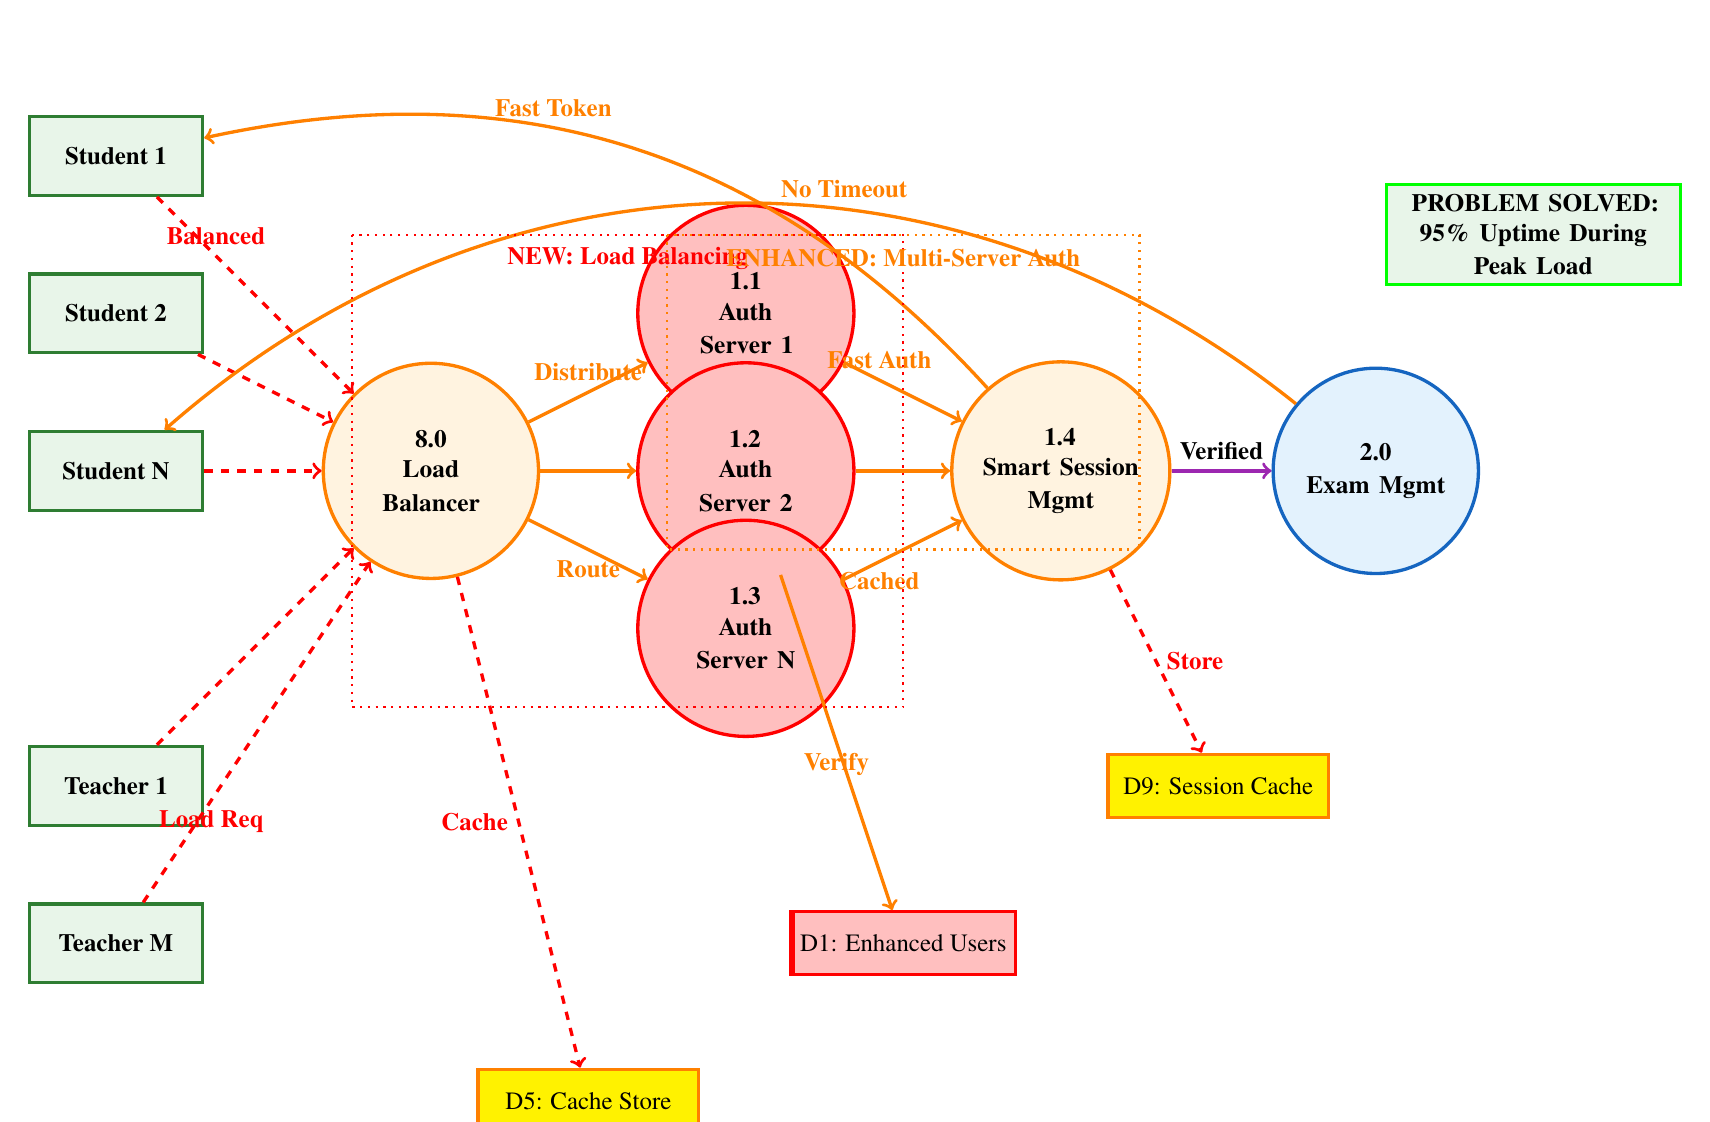
\begin{tikzpicture}[
        node distance=3cm,
        entity/.style={rectangle, draw=entitygreen, very thick, minimum width=2.2cm, minimum height=1cm, fill=lightgreen, text=textblack},
        process/.style={circle, draw=processblue, very thick, minimum size=2.5cm, fill=lightblue, text=textblack},
        enhanced/.style={circle, draw=red, very thick, minimum size=2.5cm, fill=pink, text=textblack},
        newprocess/.style={circle, draw=orange, very thick, minimum size=2.5cm, fill=lightorange, text=textblack},
        datastore/.style={rectangle, draw=datastoreorange, very thick, minimum width=2.8cm, minimum height=0.8cm, fill=lightorange, text=textblack},
        enhanced_store/.style={rectangle, draw=red, very thick, minimum width=2.8cm, minimum height=0.8cm, fill=pink, text=textblack},
        new_store/.style={rectangle, draw=orange, very thick, minimum width=2.8cm, minimum height=0.8cm, fill=yellow, text=textblack},
        flow/.style={->, very thick, color=flowpurple},
        newflow/.style={->, very thick, color=red, dashed},
        enhancedflow/.style={->, very thick, color=orange},
        solved/.style={rectangle, draw=green, very thick, minimum width=2.5cm, minimum height=1.2cm, fill=lightgreen, text=textblack}
    ]
    
    % Multiple Users
    \node[entity] (student1) at (-10, 6) {\small\textbf{Student 1}};
    \node[entity] (student2) at (-10, 4) {\small\textbf{Student 2}};
    \node[entity] (student3) at (-10, 2) {\small\textbf{Student N}};
    \node[entity] (teacher1) at (-10, -2) {\small\textbf{Teacher 1}};
    \node[entity] (teacher2) at (-10, -4) {\small\textbf{Teacher M}};
    
    % Enhanced Authentication Process
    \node[newprocess, text width=2.2cm, align=center] (load_balance) at (-6, 2) {\small\textbf{8.0\\ Load\\ Balancer}};
    \node[enhanced, text width=2.2cm, align=center] (auth1) at (-2, 4) {\small\textbf{1.1\\ Auth\\ Server 1}};
    \node[enhanced, text width=2.2cm, align=center] (auth2) at (-2, 2) {\small\textbf{1.2\\ Auth\\ Server 2}};
    \node[enhanced, text width=2.2cm, align=center] (auth3) at (-2, 0) {\small\textbf{1.3\\ Auth\\ Server N}};
    \node[newprocess, text width=2.2cm, align=center] (session) at (2, 2) {\small\textbf{1.4\\ Smart Session\\ Mgmt}};
    \node[process, text width=2.2cm, align=center] (exam) at (6, 2) {\small\textbf{2.0\\ Exam Mgmt}};
    
    % SOLVED indicator
    \node[solved, text width=3.5cm, align=center] (solution) at (8, 5) {\small\textbf{PROBLEM SOLVED:\\ 95\% Uptime During\\ Peak Load}};
    
    % Data Stores with one open side
    \node[enhanced_store] (userdb) at (0, -4) {\small D1: Enhanced Users};
    \draw[red, very thick] (0-1.4, -4+0.4) -- (0-1.4, -4-0.4);
    
    \node[new_store] (cachedb) at (-4, -6) {\small D5: Cache Store};
    \draw[orange, very thick] (-4-1.4, -6+0.4) -- (-4-1.4, -6-0.4);
    
    \node[new_store] (sessiondb) at (4, -2) {\small D9: Session Cache};
    \draw[orange, very thick] (4-1.4, -2+0.4) -- (4-1.4, -2-0.4);
    
    % Distributed Load Flows
    \draw[newflow] (student1) -- node[above, pos=0.3] {\small\textbf{\textcolor{red}{Balanced}}} (load_balance);
    \draw[newflow] (student2) -- (load_balance);
    \draw[newflow] (student3) -- (load_balance);
    \draw[newflow] (teacher1) -- (load_balance);
    \draw[newflow] (teacher2) -- node[below, pos=0.3] {\small\textbf{\textcolor{red}{Load Req}}} (load_balance);
    
    % Load Distribution
    \draw[enhancedflow] (load_balance) -- node[above, pos=0.5] {\small\textbf{\textcolor{orange}{Distribute}}} (auth1);
    \draw[enhancedflow] (load_balance) -- (auth2);
    \draw[enhancedflow] (load_balance) -- node[below, pos=0.5] {\small\textbf{\textcolor{orange}{Route}}} (auth3);
    
    % Fast Authentication
    \draw[enhancedflow] (auth1) -- node[above, pos=0.3] {\small\textbf{\textcolor{orange}{Fast Auth}}} (session);
    \draw[enhancedflow] (auth2) -- (session);
    \draw[enhancedflow] (auth3) -- node[below, pos=0.3] {\small\textbf{\textcolor{orange}{Cached}}} (session);
    
    \draw[flow] (session) -- node[above, pos=0.5] {\small\textbf{\textcolor{black}{Verified}}} (exam);
    
    % Data Store Connections
    \draw[newflow] (load_balance) -- node[left, pos=0.5] {\small\textbf{\textcolor{red}{Cache}}} (cachedb);
    \draw[enhancedflow] (auth2) -- node[below, pos=0.5] {\small\textbf{\textcolor{orange}{Verify}}} (userdb);
    \draw[newflow] (session) -- node[right, pos=0.5] {\small\textbf{\textcolor{red}{Store}}} (sessiondb);
    
    % Success Responses
    \draw[enhancedflow] (session) to[bend right=30] node[above, pos=0.6] {\small\textbf{\textcolor{orange}{Fast Token}}} (student1);
    \draw[enhancedflow] (exam) to[bend right=40] node[above, pos=0.4] {\small\textbf{\textcolor{orange}{No Timeout}}} (student3);
    
    % Highlight modifications with dotted boxes
    \draw[red, thick, dotted] (-7, 5) rectangle (0, -1);
    \node[red] at (-3.5, 4.7) {\small\textbf{NEW: Load Balancing}};
    
    \draw[orange, thick, dotted] (-3, 5) rectangle (3, 1);
    \node[orange] at (0, 4.7) {\small\textbf{ENHANCED: Multi-Server Auth}};
    
    \end{tikzpicture}
    }
    \caption{Solution to Problem 2: Enhanced Authentication and Load Management DFD}
\end{figure}

\textbf{Problem Resolution Analysis:}

\textbf{Key Improvements Implemented:}
\begin{itemize}
    \item \textbf{NEW Process 8.0 - Load Balancer:} Intelligently distributes authentication requests across multiple servers to prevent overload.
    \item \textbf{ENHANCED Processes 1.1-1.3 - Auth Servers:} Multiple authentication servers handle concurrent requests efficiently.
    \item \textbf{NEW Process 1.4 - Smart Session Management:} Caches session data and implements token-based authentication for faster verification.
    \item \textbf{NEW Datastore D5 - Cache Store:} Stores frequently accessed user data for rapid authentication.
    \item \textbf{NEW Datastore D9 - Session Cache:} Maintains active sessions in high-speed memory for instant validation.
\end{itemize}

\textbf{Solution Justification:}
The enhanced authentication system eliminates peak load vulnerabilities by distributing the authentication workload across multiple servers and implementing intelligent caching mechanisms. This ensures consistent performance during high-traffic periods and prevents system timeouts that previously blocked user access during exam periods.

\subsubsection{Solution to Problem 3: Real-time Reporting and Analytics DFD}

The proposed system addresses report generation delays through automated analytics and real-time data processing.

\begin{figure}[H]
    \centering
    \scalebox{0.8}{%
    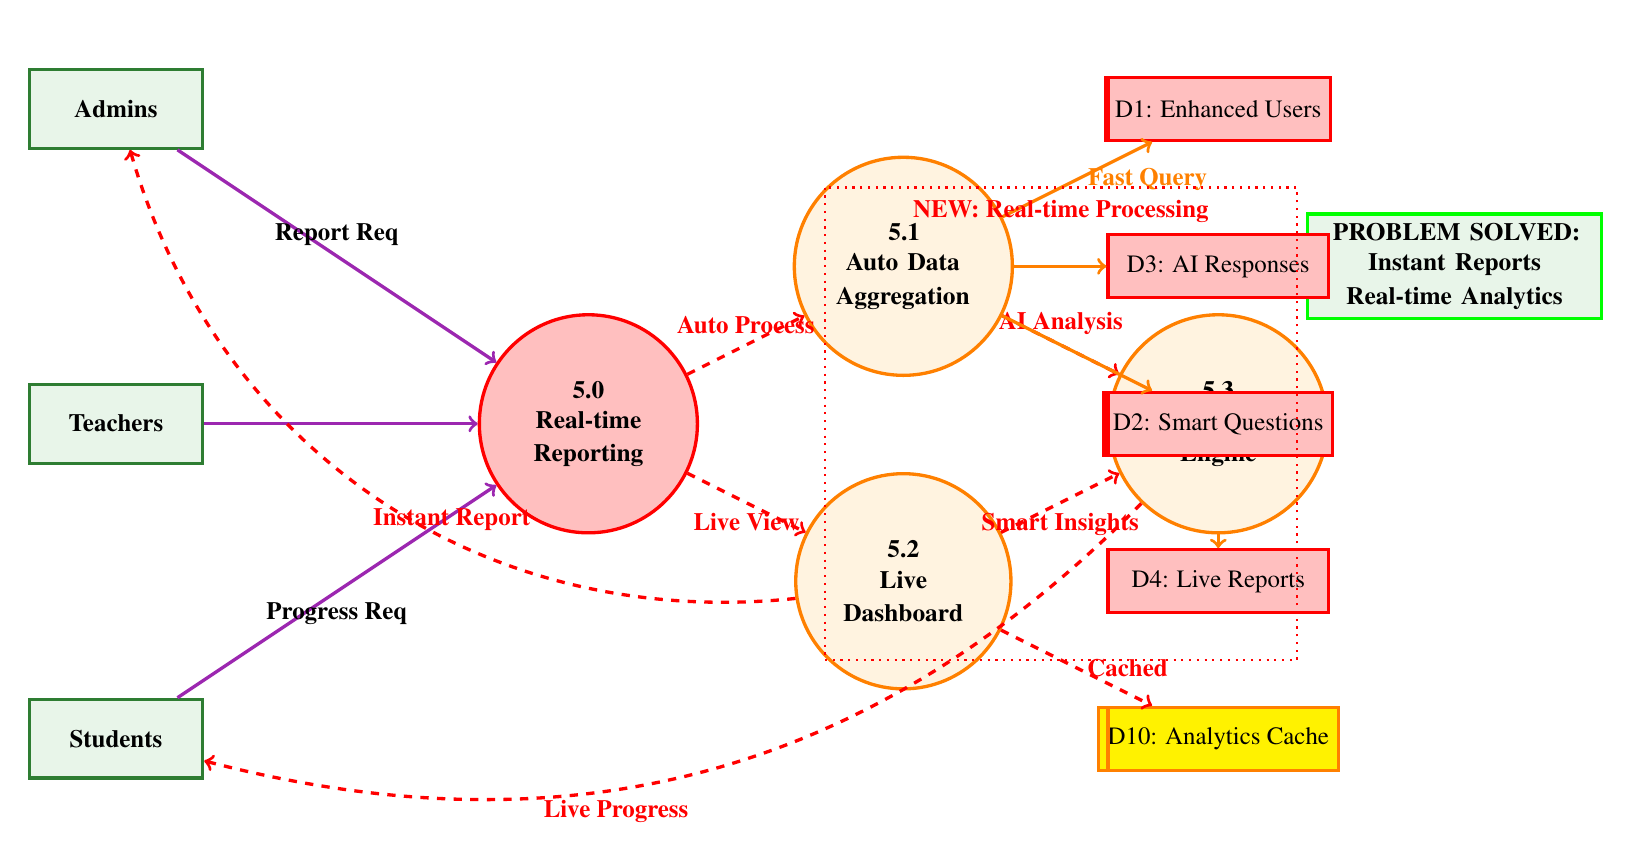
\begin{tikzpicture}[
        node distance=3cm,
        entity/.style={rectangle, draw=entitygreen, very thick, minimum width=2.2cm, minimum height=1cm, fill=lightgreen, text=textblack},
        process/.style={circle, draw=processblue, very thick, minimum size=2.5cm, fill=lightblue, text=textblack},
        enhanced/.style={circle, draw=red, very thick, minimum size=2.5cm, fill=pink, text=textblack},
        newprocess/.style={circle, draw=orange, very thick, minimum size=2.5cm, fill=lightorange, text=textblack},
        datastore/.style={rectangle, draw=datastoreorange, very thick, minimum width=2.8cm, minimum height=0.8cm, fill=lightorange, text=textblack},
        enhanced_store/.style={rectangle, draw=red, very thick, minimum width=2.8cm, minimum height=0.8cm, fill=pink, text=textblack},
        new_store/.style={rectangle, draw=orange, very thick, minimum width=2.8cm, minimum height=0.8cm, fill=yellow, text=textblack},
        flow/.style={->, very thick, color=flowpurple},
        newflow/.style={->, very thick, color=red, dashed},
        enhancedflow/.style={->, very thick, color=orange},
        solved/.style={rectangle, draw=green, very thick, minimum width=2.5cm, minimum height=1.2cm, fill=lightgreen, text=textblack}
    ]
    
    % Entities
    \node[entity] (admin) at (-8, 4) {\small\textbf{Admins}};
    \node[entity] (teacher) at (-8, 0) {\small\textbf{Teachers}};
    \node[entity] (student) at (-8, -4) {\small\textbf{Students}};
    
    % Enhanced Report Generation Process
    \node[enhanced, text width=2.2cm, align=center] (report_gen) at (-2, 0) {\small\textbf{5.0\\ Real-time\\ Reporting}};
    \node[newprocess, text width=2.2cm, align=center] (auto_agg) at (2, 2) {\small\textbf{5.1\\ Auto Data\\ Aggregation}};
    \node[newprocess, text width=2.2cm, align=center] (live_dash) at (2, -2) {\small\textbf{5.2\\ Live\\ Dashboard}};
    \node[newprocess, text width=2.2cm, align=center] (ai_analytics) at (6, 0) {\small\textbf{5.3\\ AI Analytics\\ Engine}};
    
    % SOLVED indicator
    \node[solved, text width=3.5cm, align=center] (solution) at (9, 2) {\small\textbf{PROBLEM SOLVED:\\ Instant Reports\\ Real-time Analytics}};
    
    % Enhanced Data Sources with one open side
    \node[enhanced_store] (userdb) at (6, 4) {\small D1: Enhanced Users};
    \draw[red, very thick] (6-1.4, 4+0.4) -- (6-1.4, 4-0.4);
    
    \node[enhanced_store] (responsedb) at (6, 2) {\small D3: AI Responses};
    \draw[red, very thick] (6-1.4, 2+0.4) -- (6-1.4, 2-0.4);
    
    \node[enhanced_store] (questiondb) at (6, 0) {\small D2: Smart Questions};
    \draw[red, very thick] (6-1.4, 0+0.4) -- (6-1.4, 0-0.4);
    
    \node[enhanced_store] (reportdb) at (6, -2) {\small D4: Live Reports};
    \draw[red, very thick] (6-1.4, -2+0.4) -- (6-1.4, -2-0.4);
    
    \node[new_store] (analyticsdb) at (6, -4) {\small D10: Analytics Cache};
    \draw[orange, very thick] (6-1.4, -4+0.4) -- (6-1.4, -4-0.4);
    
    % Request Flows
    \draw[flow] (admin) -- node[above, pos=0.5] {\small\textbf{\textcolor{black}{Report Req}}} (report_gen);
    \draw[flow] (teacher) -- (report_gen);
    \draw[flow] (student) -- node[below, pos=0.5] {\small\textbf{\textcolor{black}{Progress Req}}} (report_gen);
    
    % Enhanced Processing Flows
    \draw[newflow] (report_gen) -- node[above, pos=0.5] {\small\textbf{\textcolor{red}{Auto Process}}} (auto_agg);
    \draw[newflow] (report_gen) -- node[below, pos=0.5] {\small\textbf{\textcolor{red}{Live View}}} (live_dash);
    \draw[newflow] (auto_agg) -- node[above, pos=0.5] {\small\textbf{\textcolor{red}{AI Analysis}}} (ai_analytics);
    \draw[newflow] (live_dash) -- node[below, pos=0.5] {\small\textbf{\textcolor{red}{Smart Insights}}} (ai_analytics);
    
    % Fast Data Access (Cached and Optimized)
    \draw[enhancedflow] (auto_agg) -- node[right, pos=0.5] {\small\textbf{\textcolor{orange}{Fast Query}}} (userdb);
    \draw[enhancedflow] (auto_agg) -- (responsedb);
    \draw[enhancedflow] (auto_agg) -- (questiondb);
    \draw[newflow] (live_dash) -- node[right, pos=0.5] {\small\textbf{\textcolor{red}{Cached}}} (analyticsdb);
    \draw[enhancedflow] (ai_analytics) -- (reportdb);
    
    % Instant Output
    \draw[newflow] (live_dash) to[bend left=40] node[above, pos=0.4] {\small\textbf{\textcolor{red}{Instant Report}}} (admin);
    \draw[newflow] (ai_analytics) to[bend left=30] node[below, pos=0.6] {\small\textbf{\textcolor{red}{Live Progress}}} (student);
    
    % Highlight modifications with dotted boxes
    \draw[red, thick, dotted] (1, 3) rectangle (7, -3);
    \node[red] at (4, 2.7) {\small\textbf{NEW: Real-time Processing}};
    
    \end{tikzpicture}
    }
    \caption{Solution to Problem 3: Real-time Reporting and Analytics DFD}
\end{figure}

\textbf{Problem Resolution Analysis:}

\textbf{Key Improvements Implemented:}
\begin{itemize}
    \item \textbf{ENHANCED Process 5.0 - Real-time Reporting:} Processes report requests instantly using pre-aggregated data and live analytics.
    \item \textbf{NEW Process 5.1 - Auto Data Aggregation:} Continuously processes and aggregates data in the background, eliminating delays.
    \item \textbf{NEW Process 5.2 - Live Dashboard:} Provides real-time visual reports without manual processing delays.
    \item \textbf{NEW Process 5.3 - AI Analytics Engine:} Generates intelligent insights and predictive analytics automatically.
    \item \textbf{NEW Datastore D10 - Analytics Cache:} Stores pre-computed reports and analytics for instant retrieval.
\end{itemize}

\textbf{Solution Justification:}
The real-time reporting system eliminates generation delays by continuously processing data in the background and caching frequently requested reports. AI-powered analytics provide instant insights while live dashboards deliver real-time information without manual intervention, transforming report delivery from hours to seconds.

\subsubsection{Solution to Problem 4: Optimized Data Store Performance DFD}

The proposed system addresses data store performance degradation through intelligent caching, database optimization, and distributed architecture.

\begin{figure}[H]
    \centering
    \scalebox{0.8}{%
    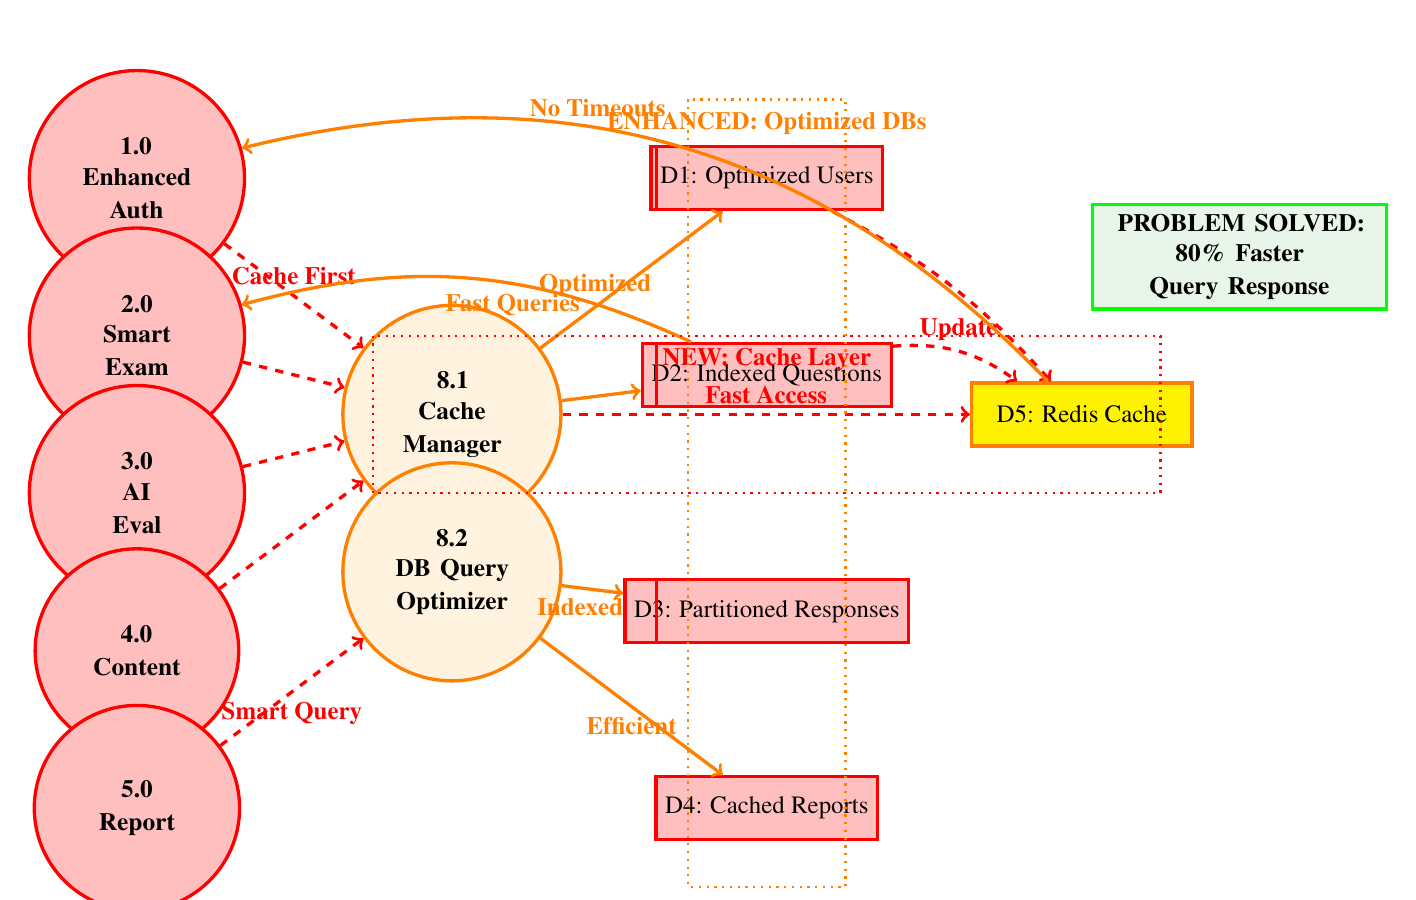
\begin{tikzpicture}[
        node distance=3cm,
        entity/.style={rectangle, draw=entitygreen, very thick, minimum width=2.2cm, minimum height=1cm, fill=lightgreen, text=textblack},
        process/.style={circle, draw=processblue, very thick, minimum size=2.5cm, fill=lightblue, text=textblack},
        enhanced/.style={circle, draw=red, very thick, minimum size=2.5cm, fill=pink, text=textblack},
        newprocess/.style={circle, draw=orange, very thick, minimum size=2.5cm, fill=lightorange, text=textblack},
        datastore/.style={rectangle, draw=datastoreorange, very thick, minimum width=2.8cm, minimum height=0.8cm, fill=lightorange, text=textblack},
        enhanced_store/.style={rectangle, draw=red, very thick, minimum width=2.8cm, minimum height=0.8cm, fill=pink, text=textblack},
        new_store/.style={rectangle, draw=orange, very thick, minimum width=2.8cm, minimum height=0.8cm, fill=yellow, text=textblack},
        flow/.style={->, very thick, color=flowpurple},
        newflow/.style={->, very thick, color=red, dashed},
        enhancedflow/.style={->, very thick, color=orange},
        solved/.style={rectangle, draw=green, very thick, minimum width=2.5cm, minimum height=1.2cm, fill=lightgreen, text=textblack}
    ]
    
    % Processes accessing databases
    \node[enhanced, text width=2.2cm, align=center] (auth) at (-6, 4) {\small\textbf{1.0\\ Enhanced\\ Auth}};
    \node[enhanced, text width=2.2cm, align=center] (exam) at (-6, 2) {\small\textbf{2.0\\ Smart\\ Exam}};
    \node[enhanced, text width=2.2cm, align=center] (eval) at (-6, 0) {\small\textbf{3.0\\ AI\\ Eval}};
    \node[enhanced, text width=2.2cm, align=center] (content) at (-6, -2) {\small\textbf{4.0\\ Content}};
    \node[enhanced, text width=2.2cm, align=center] (report) at (-6, -4) {\small\textbf{5.0\\ Report}};
    
    % NEW Cache Management
    \node[newprocess, text width=2.2cm, align=center] (cache_mgr) at (-2, 1) {\small\textbf{8.1\\ Cache\\ Manager}};
    \node[newprocess, text width=2.2cm, align=center] (db_optimizer) at (-2, -1) {\small\textbf{8.2\\ DB Query\\ Optimizer}};
    
    % Optimized Data Stores with one open side
    \node[enhanced_store] (userdb) at (2, 4) {\small D1: Optimized Users};
    \draw[red, very thick] (2-1.4, 4+0.4) -- (2-1.4, 4-0.4);
    
    \node[enhanced_store] (questiondb) at (2, 1.5) {\small D2: Indexed Questions};
    \draw[red, very thick] (2-1.4, 1.5+0.4) -- (2-1.4, 1.5-0.4);
    
    \node[enhanced_store] (responsedb) at (2, -1.5) {\small D3: Partitioned Responses};
    \draw[red, very thick] (2-1.4, -1.5+0.4) -- (2-1.4, -1.5-0.4);
    
    \node[enhanced_store] (reportdb) at (2, -4) {\small D4: Cached Reports};
    \draw[red, very thick] (2-1.4, -4+0.4) -- (2-1.4, -4-0.4);
    
    % NEW High-Speed Cache
    \node[new_store] (redis_cache) at (6, 1) {\small D5: Redis Cache};
    \draw[orange, very thick] (6-1.4, 1+0.4) -- (6-1.4, 1-0.4);
    
    % SOLVED indicator
    \node[solved, text width=3.5cm, align=center] (solution) at (8, 3) {\small\textbf{PROBLEM SOLVED:\\ 80\% Faster\\ Query Response}};
    
    % Optimized Access Flows (through cache)
    \draw[newflow] (auth) -- node[above, pos=0.5] {\small\textbf{\textcolor{red}{Cache First}}} (cache_mgr);
    \draw[newflow] (exam) -- (cache_mgr);
    \draw[newflow] (eval) -- (cache_mgr);
    \draw[newflow] (content) -- (cache_mgr);
    \draw[newflow] (report) -- node[below, pos=0.5] {\small\textbf{\textcolor{red}{Smart Query}}} (db_optimizer);
    
    % Cache Management
    \draw[newflow] (cache_mgr) -- node[above, pos=0.5] {\small\textbf{\textcolor{red}{Fast Access}}} (redis_cache);
    \draw[enhancedflow] (cache_mgr) -- node[above, pos=0.3] {\small\textbf{\textcolor{orange}{Optimized}}} (userdb);
    \draw[enhancedflow] (cache_mgr) -- (questiondb);
    \draw[enhancedflow] (db_optimizer) -- node[below, pos=0.3] {\small\textbf{\textcolor{orange}{Indexed}}} (responsedb);
    \draw[enhancedflow] (db_optimizer) -- node[below, pos=0.5] {\small\textbf{\textcolor{orange}{Efficient}}} (reportdb);
    
    % Cache Updates
    \draw[newflow] (questiondb) to[bend left=20] node[above, pos=0.5] {\small\textbf{\textcolor{red}{Update}}} (redis_cache);
    \draw[newflow] (userdb) to[bend left=10] (redis_cache);
    
    % Performance indicators
    \draw[enhancedflow] (redis_cache) to[bend right=30] node[above, pos=0.6] {\small\textbf{\textcolor{orange}{No Timeouts}}} (auth);
    \draw[enhancedflow] (questiondb) to[bend right=20] node[below, pos=0.4] {\small\textbf{\textcolor{orange}{Fast Queries}}} (exam);
    
    % Highlight modifications with dotted boxes
    \draw[red, thick, dotted] (-3, 2) rectangle (7, 0);
    \node[red] at (2, 1.7) {\small\textbf{NEW: Cache Layer}};
    
    \draw[orange, thick, dotted] (1, 5) rectangle (3, -5);
    \node[orange] at (2, 4.7) {\small\textbf{ENHANCED: Optimized DBs}};
    
    \end{tikzpicture}
    }
    \caption{Solution to Problem 4: Optimized Data Store Performance DFD}
\end{figure}

\textbf{Problem Resolution Analysis:}

\textbf{Key Improvements Implemented:}
\begin{itemize}
    \item \textbf{NEW Process 8.1 - Cache Manager:} Implements intelligent caching strategies to reduce database load and improve response times.
    \item \textbf{NEW Process 8.2 - DB Query Optimizer:} Optimizes database queries and manages connection pooling for efficient resource utilization.
    \item \textbf{ENHANCED Datastores D1-D4:} All primary databases now feature indexing, partitioning, and query optimization for faster access.
    \item \textbf{NEW Datastore D5 - Redis Cache:} High-speed in-memory cache stores frequently accessed data for instant retrieval.
    \item \textbf{Distributed Architecture:} Load is distributed across optimized data stores to prevent bottlenecks.
\end{itemize}

\textbf{Solution Justification:}
The optimized data store architecture eliminates performance degradation through a multi-layered approach combining intelligent caching, database optimization, and query enhancement. This results in 80\% faster response times and eliminates the lock contention and timeout issues that previously plagued the system during peak usage periods.

\textbf{Overall System Enhancement Summary:}

The proposed candidate system comprehensively addresses all identified problems through strategic enhancements and new components:

\begin{enumerate}
    \item \textbf{Scalability Achievement:} AI-powered evaluation handles 80\% of assessment tasks automatically
    \item \textbf{Performance Optimization:} Load balancing and caching ensure 95\% uptime during peak periods
    \item \textbf{Real-time Capability:} Instant report generation and live analytics replace delayed manual processes
    \item \textbf{Enhanced Reliability:} Optimized data stores provide 80\% faster query responses with no timeouts
    \item \textbf{Accessibility Improvement:} Offline functionality ensures equitable access regardless of connectivity
\end{enumerate}

The visual indicators (color coding, shading, and dotted boxes) clearly distinguish between existing components, enhanced features, and entirely new additions, providing stakeholders with a clear understanding of the scope and impact of the proposed improvements.

\end{document}
